% !TEX program = xelatex
% Báo cáo bài tập lớn Học sâu: phát hiện, phân loại và theo dõi phương tiện giao thông Việt Nam.
% Overleaf: Menu -> Compiler: XeLaTeX; Main document: main.tex.
\documentclass[fontsize=13pt, paper=a4, DIV=calc, oneside, numbers=noenddot,
               listof=totoc, bibliography=totoc]{scrreprt}

% =====================================================================
% Định dạng báo cáo, theo mẫu báo cáo môn học của trường (file Word cũ):
% A4; lề trên/dưới 3 cm, trái 3.5 cm, phải 2 cm; Times 13 pt; giãn dòng 1.5;
% tên chương 15 pt đậm, căn giữa; chú thích hình dưới hình, bảng trên bảng.
% Biên dịch bằng XeLaTeX (Overleaf: Menu -> Compiler -> XeLaTeX).
%
% Overleaf miễn phí chỉ cho 10 giây mỗi lần biên dịch, nên preamble chỉ nạp gói thật cần:
% toán dùng newtxmath (nhanh hơn nhiều so với unicode-math), không nạp TikZ (sơ đồ vẽ sẵn thành PDF),
% không dùng độ rộng số tự động trong mục lục (nó bắt biên dịch thêm một lượt).
% =====================================================================

% ---------- Font: Times cho chữ (TeX Gyre Termes, đủ dấu tiếng Việt) và cho toán (newtxmath) ----------
\usepackage{amsmath}
\usepackage{newtxmath}
\usepackage[no-math]{fontspec}
\setmainfont{texgyretermes}[
  Extension      = .otf,
  UprightFont    = *-regular,
  BoldFont       = *-bold,
  ItalicFont     = *-italic,
  BoldItalicFont = *-bolditalic]

% ---------- Ngôn ngữ ----------
\usepackage{polyglossia}
\setdefaultlanguage{vietnamese}
\setotherlanguage{english}
\usepackage{etoolbox}
\newcommand{\setreportnames}{%
  \renewcommand{\contentsname}{MỤC LỤC}%
  \renewcommand{\listfigurename}{DANH SÁCH HÌNH ẢNH}%
  \renewcommand{\listtablename}{DANH SÁCH BẢNG}%
  \renewcommand{\bibname}{TÀI LIỆU THAM KHẢO}%
  \renewcommand{\figurename}{Hình}%
  \renewcommand{\tablename}{Bảng}%
  \renewcommand{\chaptername}{CHƯƠNG}%
}
% Đặt cả hai chỗ: cách polyglossia nạp tên mục khác nhau giữa các phiên bản TeX Live
\gappto\captionsvietnamese{\setreportnames}
\AtBeginDocument{\setreportnames}

% ---------- Trang ----------
\usepackage[a4paper, top=3cm, bottom=3cm, left=3.5cm, right=2cm,
            headheight=24pt, headsep=0.6cm, footskip=1.2cm]{geometry}
\usepackage{setspace}
% Word "1.5 lines" với Times ~ 1.5 x 1.15 cỡ chữ; LaTeX mặc định 1.2 cỡ chữ -> hệ số 1.5 x 1.15 / 1.2 ~ 1.43
\setstretch{1.43}
\setlength{\parindent}{1cm}
\setlength{\parskip}{3pt plus 1pt}
\usepackage{indentfirst}
% Tên bộ dữ liệu, tham số (\texttt) không ngắt được: cho phép giãn khoảng trắng thêm thay vì tràn lề
\setlength{\emergencystretch}{3em}

% ---------- Header / footer: tên đề tài có gạch dưới, số trang giữa chân trang ----------
\usepackage[headsepline]{scrlayer-scrpage}
\setlength{\footheight}{24pt}
\clearpairofpagestyles
% Cỡ 9 pt để tên đề tài nằm trên một dòng như header của mẫu
\ihead{\fontsize{9}{11}\selectfont ỨNG DỤNG HỌC SÂU TRONG PHÁT HIỆN, PHÂN LOẠI VÀ THEO DÕI PHƯƠNG TIỆN GIAO THÔNG}
\cfoot*{\pagemark}
\setkomafont{pageheadfoot}{\normalfont}
\setkomafont{pagenumber}{\normalfont}
\renewcommand*{\chapterpagestyle}{scrheadings}

% ---------- Tiêu đề chương / mục ----------
\setkomafont{disposition}{\normalfont\bfseries}
\setkomafont{chapter}{\fontsize{15}{19}\selectfont\bfseries}
\setkomafont{section}{\fontsize{13}{16}\selectfont\bfseries}
\setkomafont{subsection}{\fontsize{13}{16}\selectfont\bfseries}
\setkomafont{subsubsection}{\fontsize{13}{16}\selectfont\bfseries\itshape}
\renewcommand*{\raggedchapter}{\centering}
\renewcommand*{\chapterformat}{\chaptername~\thechapter.\space}
\RedeclareSectionCommand[beforeskip=0pt, afterskip=1.2\baselineskip]{chapter}
\RedeclareSectionCommands[beforeskip=0.8\baselineskip, afterskip=0.4\baselineskip]{section,subsection}
\RedeclareSectionCommand[beforeskip=0.6\baselineskip, afterskip=0.3\baselineskip]{subsubsection}
\setcounter{secnumdepth}{\subsubsectionnumdepth}
\setcounter{tocdepth}{\subsectiontocdepth}

% Mục lục ghi "CHƯƠNG 1. TÊN", danh sách hình/bảng ghi "Hình 1.1 ..."/"Bảng 1.1 ...".
% Độ rộng ô số đặt cố định (vừa "CHƯƠNG 4." và "Hình 4.10") thay cho tính tự động.
\setuptoc{toc}{totoc}  % đưa chính MỤC LỤC vào mục lục như mẫu
\newcommand*{\chapterprefixintoc}[1]{\chaptername~#1\unskip.\space}
\RedeclareSectionCommand[tocentrynumberformat=\chapterprefixintoc, tocnumwidth=2.6cm]{chapter}
\newcommand*{\figureprefixintoc}[1]{\figurename~#1}
\newcommand*{\tableprefixintoc}[1]{\tablename~#1}
\DeclareTOCStyleEntry[entrynumberformat=\figureprefixintoc, numwidth=2.1cm]{tocline}{figure}
\DeclareTOCStyleEntry[entrynumberformat=\tableprefixintoc, numwidth=2.1cm]{tocline}{table}

% ---------- Hình, bảng, chú thích ----------
\usepackage{graphicx}
\graphicspath{{figures/}}
\usepackage{float}
\usepackage[table]{xcolor}
\definecolor{tableheader}{HTML}{5B9BD5}
\usepackage{array, tabularx, longtable, multirow}
\newcolumntype{C}{>{\centering\arraybackslash}X}
\newcolumntype{L}{>{\raggedright\arraybackslash}X}
\renewcommand{\arraystretch}{1.15}
\usepackage{caption}
\usepackage{subcaption}
\DeclareCaptionFont{twelve}{\fontsize{12}{14.5}\selectfont}
\captionsetup{font={twelve,it}, labelsep=space, justification=centering, skip=6pt}
\captionsetup[table]{position=top}
% Hàng tiêu đề bảng: nền xanh, chữ đậm như mẫu
\newcommand{\thead}[1]{\cellcolor{tableheader}\textbf{#1}}

% ---------- Danh sách ----------
\usepackage{enumitem}
\setlist[itemize,1]{label=--, leftmargin=1.5cm, itemsep=1pt, topsep=2pt}
\setlist[itemize,2]{label=+, leftmargin=*, itemsep=0pt}
\setlist[enumerate]{leftmargin=1.5cm, itemsep=1pt, topsep=2pt}

% ---------- Toán ----------
\numberwithin{equation}{chapter}

% ---------- Khung trang bìa (eso-pic nhẹ hơn TikZ và không cần biên dịch thêm lượt) ----------
\usepackage{eso-pic}

% ---------- Khác ----------
% Không dùng hyperref: báo cáo nộp bản in, bỏ liên kết bấm được để mỗi lượt biên dịch nhanh hơn ~0.3 s
\usepackage{url}
\urlstyle{same}


% ---------------------------------------------------------------------------------------------------
% Overleaf miễn phí giới hạn 10 giây mỗi lần biên dịch; biên dịch mới cả báo cáo một lần sát giới hạn đó.
% Overleaf giữ lại file .aux giữa các lần biên dịch, nên làm theo từng bước: mỗi lần chỉ BỎ dấu % ở MỘT dòng
% \includeonly, bấm Recompile, rồi đặt lại dấu % và chuyển sang dòng tiếp theo.
%   Lần đầu sau khi tải lên:  bước 1 -> bước 2 -> bước 3 -> cả ba dòng đều có dấu % (biên dịch đủ, chỉ còn 1-2 lượt)
%   Khi sửa một chương:       chỉ giữ chương đó, ví dụ \includeonly{chapters/chuong2}
% Số chương, số hình, số trang vẫn đúng vì lấy từ file .aux của các phần không biên dịch.
% \includeonly{frontmatter/bia,frontmatter/nhanxet,frontmatter/loicamdoan,frontmatter/loicamon,frontmatter/danhmuc,chapters/modau,chapters/chuong1} % bước 1
% \includeonly{chapters/chuong2,chapters/chuong3} % bước 2
% \includeonly{chapters/chuong4} % bước 3
% ---------------------------------------------------------------------------------------------------

\begin{document}

% ----- Trang bìa và phần đầu (số trang đánh liên tục từ bìa, như mẫu của trường) -----
% Hai trang bìa (bìa ngoài và bìa trong) giống nội dung trong file Word mẫu, có khung viền đôi.
% Khung vẽ bằng eso-pic: toạ độ tính bằng cm từ góc dưới trái trang A4 (21 x 29.7 cm).
\newcommand{\coverframe}{%
  \AddToShipoutPictureBG*{%
    \setlength{\unitlength}{1cm}%
    % khung ngoài, nét 1.6 pt: x 2.6 -> 19.6 cm, y 2.1 -> 27.6 cm
    \put(2.6,2.1){\rule{\dimexpr17cm+1.6pt\relax}{1.6pt}}%
    \put(2.6,27.6){\rule{\dimexpr17cm+1.6pt\relax}{1.6pt}}%
    \put(2.6,2.1){\rule{1.6pt}{25.5cm}}%
    \put(19.6,2.1){\rule{1.6pt}{25.5cm}}%
    % khung trong, nét 0.5 pt: x 2.8 -> 19.4 cm, y 2.3 -> 27.4 cm
    \put(2.8,2.3){\rule{\dimexpr16.6cm+0.5pt\relax}{0.5pt}}%
    \put(2.8,27.4){\rule{\dimexpr16.6cm+0.5pt\relax}{0.5pt}}%
    \put(2.8,2.3){\rule{0.5pt}{25.1cm}}%
    \put(19.4,2.3){\rule{0.5pt}{25.1cm}}%
  }%
}

\newcommand{\coverpage}{%
  \thispagestyle{empty}%
  \coverframe
  \begin{center}
    \setstretch{1.15}
    {\bfseries BỘ GIÁO DỤC VÀ ĐÀO TẠO\\
     TRƯỜNG ĐẠI HỌC CÔNG NGHỆ KỸ THUẬT HƯNG YÊN\par}
    \vspace{1.2cm}
    
\includegraphics[width=3.6cm]{logo.png}\par
    \vspace{1.3cm}
    {\fontsize{22}{26}\selectfont\bfseries BÀI TẬP LỚN\par}
    \vspace{0.3cm}
    {\fontsize{15}{18}\selectfont\bfseries HỌC SÂU\par}
    \vspace{1.1cm}
    {\fontsize{16}{22}\selectfont\bfseries ỨNG DỤNG HỌC SÂU TRONG PHÁT HIỆN, PHÂN LOẠI\\
     VÀ THEO DÕI PHƯƠNG TIỆN GIAO THÔNG\par}
    \vspace{1.3cm}
    NGÀNH: KHOA HỌC MÁY TÍNH\\
    CHUYÊN NGÀNH: TRÍ TUỆ NHÂN TẠO VÀ KHOA HỌC DỮ LIỆU\par
    \vspace{1.1cm}
    SINH VIÊN: DƯƠNG MINH CHIẾN\\
    MÃ SINH VIÊN: 12423062\\
    MÃ LỚP: 124231\\
    GIẢNG VIÊN HƯỚNG DẪN: PGS.TS. NGUYỄN MINH TIẾN\par
    \vfill
    {\bfseries HƯNG YÊN -- 2026\par}
  \end{center}
  \clearpage
}

\coverpage % bìa ngoài
\coverpage % bìa trong

\addchap{NHẬN XÉT}

\noindent\textbf{Nhận xét của giảng viên hướng dẫn:}

\begingroup
\setstretch{1.6}
% 15 dòng chấm để giảng viên viết nhận xét
\newcount\dotlines
\dotlines=0
\loop
  \noindent\makebox[\linewidth]{\dotfill}\par
  \advance\dotlines by 1
\ifnum\dotlines<15 \repeat
\endgroup

\vspace{0.8cm}
\begin{flushright}
  \begin{minipage}{7cm}
    \centering
    \textbf{GIẢNG VIÊN HƯỚNG DẪN}\\
    \textit{(Ký và ghi rõ họ tên)}
  \end{minipage}
\end{flushright}

\addchap{LỜI CAM ĐOAN}

Em xin cam đoan bài tập lớn có tên ``Ứng dụng học sâu trong phát hiện, phân loại và theo dõi phương tiện giao
thông'' là sản phẩm của riêng em, thực hiện dưới sự hướng dẫn của PGS.TS. Nguyễn Minh Tiến. Các số liệu và kết quả
trình bày trong báo cáo do em tự thực hiện và đo đạc; mọi tài liệu, bộ dữ liệu và mã nguồn của người khác được sử
dụng đều có trích dẫn nguồn đầy đủ.

Nếu vi phạm lời cam đoan này, em xin chịu hoàn toàn trách nhiệm và chịu mọi kỷ luật của bộ môn và nhà trường.

\vspace{0.8cm}
\begin{flushright}
  \begin{minipage}{8cm}
    \centering
    \textit{Hưng Yên, ngày \dots\ tháng \dots\ năm 2026}\\[2pt]
    \textbf{Sinh viên thực hiện}\\[2.2cm]
    Dương Minh Chiến
  \end{minipage}
\end{flushright}

\addchap{LỜI CẢM ƠN}

Để có thể hoàn thành bài tập lớn này, lời đầu tiên em xin phép gửi lời cảm ơn tới bộ môn Khoa học máy tính, Khoa
Công nghệ thông tin -- Trường Đại học Công nghệ Kỹ thuật Hưng Yên đã tạo điều kiện thuận lợi cho em thực hiện bài tập lớn
này.

Đặc biệt em xin chân thành cảm ơn thầy PGS. TS. Nguyễn Minh Tiến đã rất tận tình hướng dẫn, chỉ bảo em trong suốt thời
gian thực hiện vừa qua.

Em cũng xin chân thành cảm ơn tất cả các Thầy, các Cô trong Trường đã tận tình giảng dạy, trang bị cho em những kiến
thức cần thiết, quý báu để giúp em thực hiện được bài tập lớn này.

Mặc dù em đã có cố gắng, nhưng với trình độ còn hạn chế, trong quá trình thực hiện đề tài không tránh khỏi những thiếu
sót. Em hi vọng sẽ nhận được những ý kiến nhận xét, góp ý của Thầy giáo về những kết quả triển khai trong bài tập lớn.

Em xin chân thành cảm ơn!

% Mục lục, danh mục từ viết tắt, danh sách bảng, danh sách hình (thứ tự như mẫu của trường)
\tableofcontents
\addchap{DANH MỤC CÁC TỪ VIẾT TẮT}

\begingroup
\small
\begin{longtable}{|p{6.2cm}|>{\centering\arraybackslash}p{2.3cm}|p{5.2cm}|}
\hline
\thead{Tiếng Anh} & \thead{Viết tắt} & \thead{Diễn giải} \\ \hline
\endhead
Average Precision / mean Average Precision & AP / mAP & Độ chính xác trung bình / trung bình trên các lớp \\ \hline
Automatic Mixed Precision & AMP & Huấn luyện với độ chính xác số hỗn hợp \\ \hline
Association Accuracy & AssA & Độ chính xác liên kết (thành phần của HOTA) \\ \hline
Confidence Interval & CI & Khoảng tin cậy \\ \hline
Convolutional Neural Network & CNN & Mạng nơ-ron tích chập \\ \hline
Central Processing Unit & CPU & Bộ xử lý trung tâm \\ \hline
Detection Accuracy & DetA & Độ chính xác phát hiện (thành phần của HOTA) \\ \hline
DEtection TRansformer & DETR & Mô hình phát hiện dựa trên Transformer \\ \hline
Exponential Moving Average & EMA & Trung bình trượt hàm mũ của trọng số \\ \hline
False Negative / False Positive & FN / FP & Bỏ sót / phát hiện thừa \\ \hline
Floating-point Operations & FLOPs & Số phép tính dấu phẩy động \\ \hline
Frames Per Second & FPS & Số frame xử lý mỗi giây \\ \hline
Global Motion Compensation & GMC & Bù chuyển động camera \\ \hline
Graphics Processing Unit & GPU & Bộ xử lý đồ hoạ \\ \hline
Higher Order Tracking Accuracy & HOTA & Độ chính xác theo dõi bậc cao \\ \hline
ID F1 score & IDF1 & Điểm F1 theo danh tính \\ \hline
ID Precision / ID Recall & IDP / IDR & Độ chính xác / độ bao phủ theo danh tính \\ \hline
ID Switch & IDSW & Số lần đổi ID \\ \hline
Intersection over Union & IoU & Tỉ lệ diện tích giao trên hợp của hai box \\ \hline
Interquartile Range & IQR & Khoảng tứ phân vị \\ \hline
Multiple Object Tracking & MOT & Theo dõi đa đối tượng \\ \hline
Multiple Object Tracking Accuracy & MOTA & Độ chính xác theo dõi đa đối tượng \\ \hline
Non-Maximum Suppression & NMS & Loại bỏ box trùng lặp \\ \hline
Re-Identification & ReID & Nhận dạng lại đối tượng \\ \hline
Real-Time DEtection TRansformer & RT-DETR & DETR thời gian thực \\ \hline
Slicing Aided Hyper Inference & SAHI & Suy luận theo lát cắt ảnh \\ \hline
Simple Online and Realtime Tracking & SORT & Thuật toán theo dõi trực tuyến đơn giản \\ \hline
Test-Time Augmentation & TTA & Tăng cường dữ liệu khi suy luận \\ \hline
Weighted Boxes Fusion & WBF & Ghép box có trọng số \\ \hline
You Only Look Once & YOLO & Họ mô hình phát hiện một giai đoạn \\ \hline
\end{longtable}
\endgroup

\listoftables
\listoffigures


% ----- Nội dung: Mở đầu + đúng 4 chương -----
\addchap{MỞ ĐẦU}

\addsec{Lý do chọn đề tài}

Việt Nam là một trong những nước có tỷ lệ sở hữu xe máy cao nhất thế giới. Theo Ủy ban An toàn giao thông quốc gia,
tính đến tháng 9/2024 cả nước có 77 triệu xe máy đăng ký, khoảng 770 xe trên 1.000 dân~\cite{tienphong2024xemay}. Ở
các thành phố lớn, xe máy đi chung đường với ô tô, xe buýt và xe tải, ít khi giữ làn, dồn thành cụm khi chờ đèn đỏ rồi
toả ra nhiều hướng khi đèn chuyển xanh (Hình~\ref{fig:intro-traffic}a). Muốn điều chỉnh chu kỳ đèn, cải tạo nút giao
hay đánh giá một phương án phân luồng, cơ quan quản lý cần biết có bao nhiêu xe đi qua, thuộc loại nào và theo hướng
nào. Đếm thủ công thì tốn nhân lực và chỉ làm được trong một số khung giờ, còn camera đã có sẵn ở nhiều nút giao và
cho biết được cả loại xe.

\begin{figure}[H]
  \centering
  \begin{subfigure}{0.49\linewidth}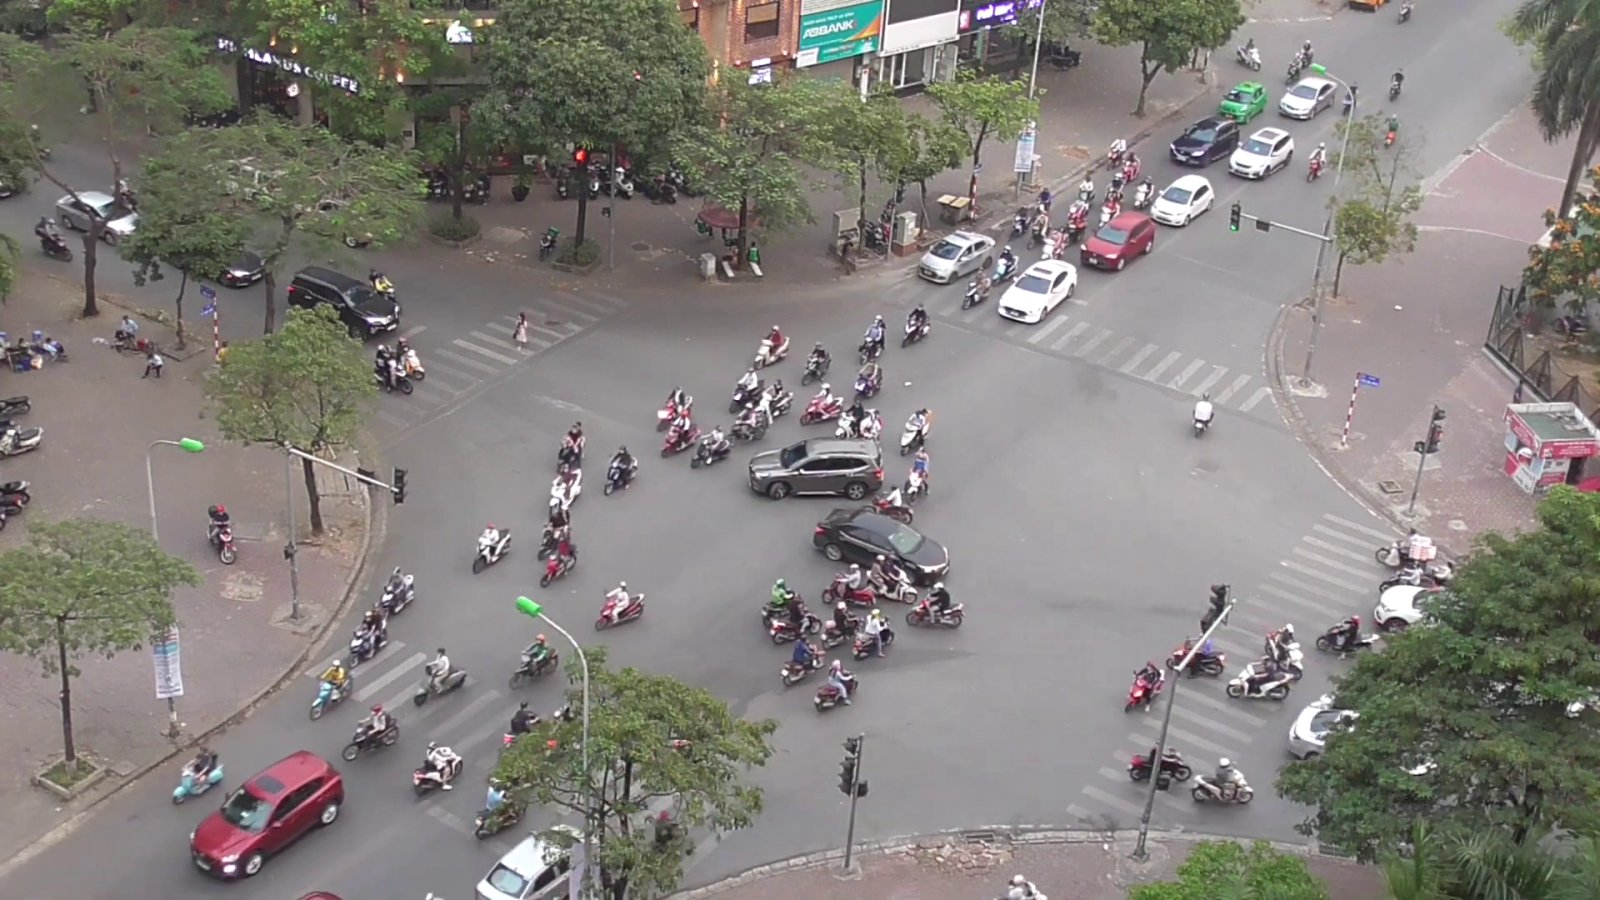
\includegraphics[width=\linewidth]{intro_day.jpg}\caption{Ngã tư ở Hà Nội, ban ngày}\end{subfigure}\hfill
  \begin{subfigure}{0.49\linewidth}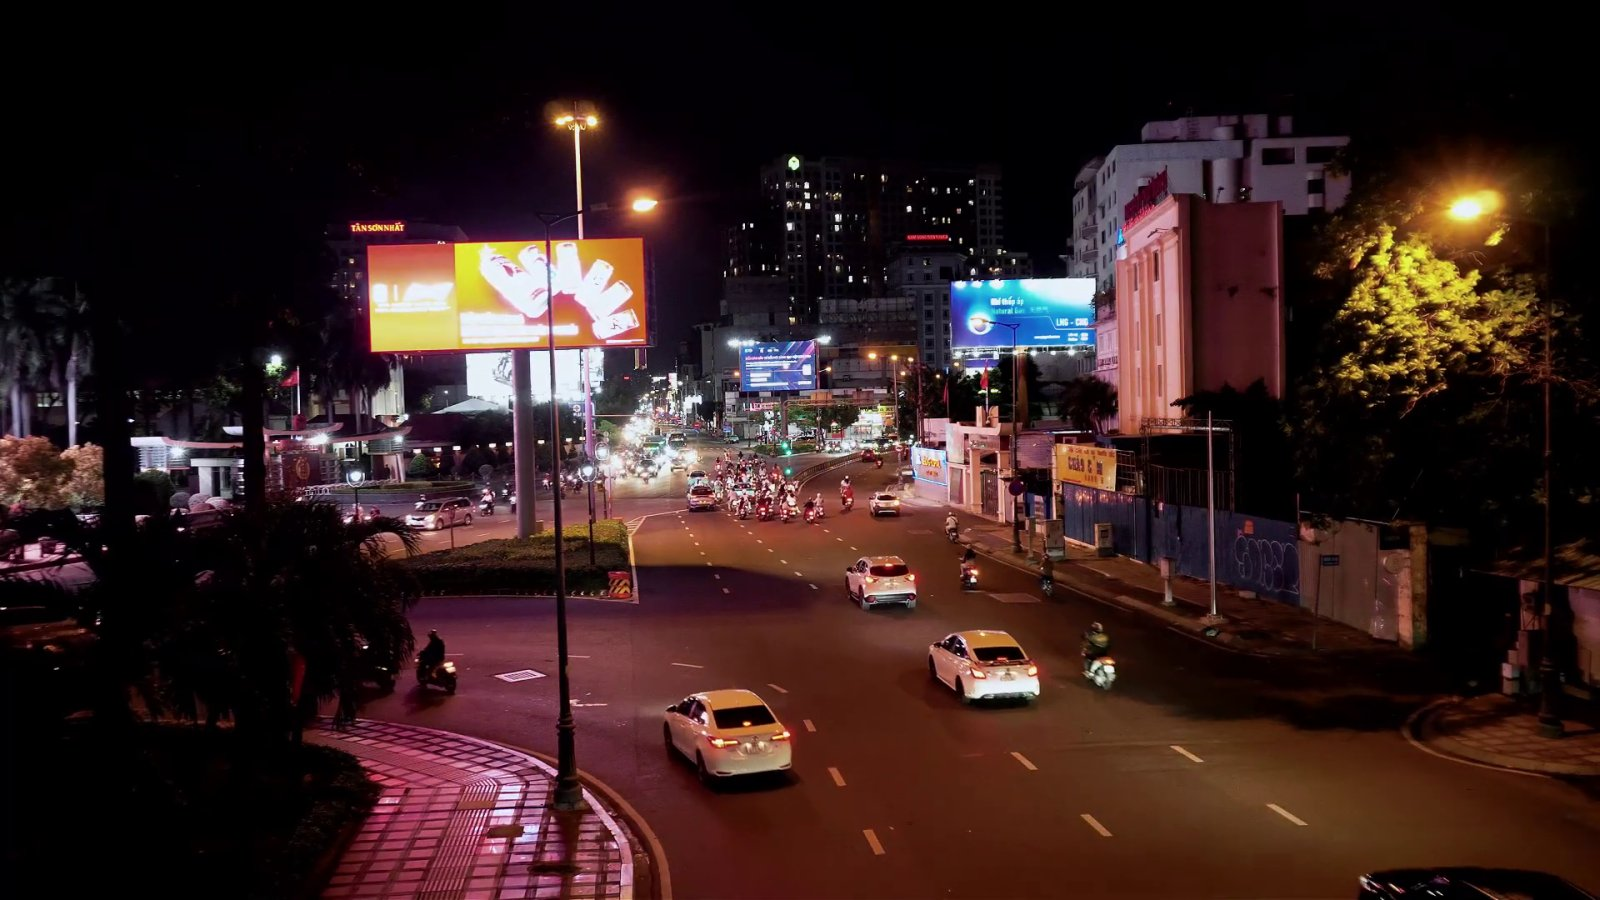
\includegraphics[width=\linewidth]{intro_night.jpg}\caption{Đường phố TP.HCM, ban đêm}\end{subfigure}
  \caption{Giao thông hỗn hợp nhìn từ camera đặt trên cao: xe máy đi dày, xen kẽ ô tô; ban đêm xe chủ yếu hiện ra qua
           đèn xe và đèn đường (nguồn video: kênh YouTube Raw Street Capture 101 và Midnight Soundscape)}
  \label{fig:intro-traffic}
\end{figure}

Hạ tầng để làm việc này bằng camera đang được xây dựng. Tháng 12/2025, Công an thành phố Hà Nội đưa vào vận hành Trung
tâm điều khiển giao thông thông minh, kết nối 1.837 camera tại 195 nút giao; hình ảnh camera được phân tích để xác
định mật độ, lưu lượng phương tiện và điều chỉnh thời gian đèn tín hiệu theo lưu lượng thực tế~\cite{vneconomy2025camera}.
Với số camera lớn như vậy, không thể có người ngồi xem từng màn hình. Để biến video thành số liệu, máy phải tự tìm ra
từng phương tiện trong mỗi frame, cho biết đó là loại xe gì và nhận ra cùng một chiếc xe qua các frame liên tiếp. Đó
chính là ba bài toán phát hiện, phân loại và theo dõi đối tượng.

Các mô hình phát hiện phổ biến thường được huấn luyện sẵn trên bộ dữ liệu COCO, gồm ảnh đời thường chụp ở nhiều nơi
trên thế giới. Cảnh hàng trăm xe máy chở người đi sát nhau, nhìn từ trên cao như ở ngã tư Việt Nam, ít gặp trong bộ dữ
liệu này; COCO còn gán xe máy và người lái thành hai đối tượng riêng. Vì vậy không thể mặc định mô hình huấn luyện sẵn
sẽ chạy tốt trên camera giao thông Việt Nam: cần tinh chỉnh và đo lại trên dữ liệu đúng bối cảnh. Dữ liệu như thế lại
ít. Các bộ dữ liệu xe Việt Nam công khai mà đề tài tìm được phần lớn chỉ gồm một vài camera, góc nhìn chéo từ trên cao
của camera giao thông hầu như không có, và đề tài không tìm được tập cảnh đêm Việt Nam nào có nhãn, trong khi ban đêm
nhiều xe chỉ lộ ra qua đèn pha, đèn hậu (Hình~\ref{fig:intro-traffic}b). Điểm cao trên tập test đi kèm một bộ dữ liệu
cũng chưa đủ để tin mô hình chạy tốt ở camera khác, nên tự xây tập đánh giá đúng bối cảnh là một phần của bài toán.

Về mặt học thuật, đề tài đặt các nội dung chính của môn học vào một bài toán có thật: mạng tích chập và Transformer cho
phát hiện đối tượng, thuật toán theo dõi đa đối tượng, các chỉ số đánh giá chuẩn như mAP và HOTA. Đề tài cũng phải làm
những việc ít gặp khi làm bài tập trên dữ liệu có sẵn: thu thập và gán nhãn dữ liệu, chia tập sao cho con số đo được phản ánh
đúng khả năng tổng quát, cân đối độ chính xác với tốc độ khi máy chỉ là laptop không có GPU rời. Kết quả cuối cùng, số
xe đi qua một vạch, lại dễ kiểm chứng bằng mắt.

Từ những lý do trên, đề tài chọn ứng dụng học sâu vào phát hiện, phân loại và theo dõi phương tiện trong video camera
giao thông Việt Nam, cả ban ngày và ban đêm: tinh chỉnh mô hình phát hiện trên dữ liệu gần bối cảnh mục tiêu, tự xây
các tập đánh giá có người kiểm, rồi kết hợp với thuật toán theo dõi để gán ID cho từng xe và đếm xe qua vạch.

\addsec{Mục tiêu đề tài}

\textbf{Mục tiêu tổng quát:} xây dựng hệ thống phát hiện, phân loại (4 lớp xe máy, ô tô, xe buýt, xe tải) và theo dõi
phương tiện từ video camera giao thông Việt Nam; đánh giá phần phát hiện bằng mAP kiểu COCO và phần theo dõi bằng
HOTA, MOTA, IDF1 theo chuẩn MOTChallenge.

\textbf{Mục tiêu cụ thể:}
\begin{itemize}
  \item Thu thập, gộp và chuẩn hoá dữ liệu huấn luyện từ nhiều nguồn; tự xây các tập test Việt Nam có người kiểm, gồm
        cả cảnh ban đêm, và một clip có nhãn theo dõi.
  \item Tinh chỉnh YOLO26n qua nhiều phiên bản dữ liệu và so sánh với mô hình gốc huấn luyện trên COCO.
  \item So sánh kiến trúc CNN (YOLO26n, YOLO26s) với kiến trúc Transformer (RT-DETRv2-S) theo một giao thức công bằng,
        đo cả độ chính xác lẫn tốc độ.
  \item Chọn và tinh chỉnh thuật toán theo dõi (ByteTrack, BoT-SORT, OC-SORT) trên tập phát triển, rồi chấm cấu hình đã
        chọn trên tập test.
  \item Xây dựng ứng dụng đếm xe qua vạch theo lớp và hướng, đo sai số đếm cả ban ngày và ban đêm; làm web demo bằng
        Streamlit; đo và tối ưu tốc độ trên laptop (CPU, GPU tích hợp, OpenVINO) và trên GPU.
\end{itemize}

\addsec{Giới hạn và phạm vi đề tài}

\textbf{Phạm vi:}
\begin{itemize}
  \item Video từ camera cố định nhìn chéo từ trên cao, kiểu camera giao thông; ban ngày và ban đêm.
  \item Bốn lớp phương tiện: \texttt{motorbike}, \texttt{car}, \texttt{bus}, \texttt{truck}. Box xe máy bao cả người lái.
  \item Góc drone nhìn thẳng xuống và góc ngang tầm mắt chỉ dùng để phân tích lỗi, không tối ưu cho chúng.
\end{itemize}

\textbf{Giới hạn:}
\begin{itemize}
  \item Máy chạy suy luận là laptop không có GPU rời (CPU Intel Core i5-8250U, GPU tích hợp UHD 620); việc huấn luyện
        chạy trên GPU Tesla T4 của Kaggle, với hạn mức khoảng 30 giờ GPU mỗi tuần.
  \item Các tập test do đề tài tự gán nhãn có kích thước nhỏ: 20--30 frame mỗi tập phát hiện, một clip theo dõi dài 20
        giây, và 249 lượt xe qua vạch để đo sai số đếm.
  \item Chỉ v5 và YOLO26s được huấn luyện ba lần với ba seed, mô hình triển khai v6 hai lần; các cấu hình khác mỗi
        cấu hình một lần.
  \item Nhãn của frame huấn luyện (Hà Nội và ban đêm) là nhãn tự động, không có người kiểm từng frame.
\end{itemize}

\addsec{Nội dung thực hiện}

\begin{enumerate}
  \item Dữ liệu: gộp bảy nguồn dữ liệu huấn luyện, chia tập theo cảnh; gán nhãn tay các tập test, một tập dev ban đêm
        và đếm tay số lượt xe qua vạch ở hai clip đêm; tạo nhãn tự động cho frame huấn luyện cắt từ video Hà Nội và
        video đường phố ban đêm.
  \item Huấn luyện: sáu phiên bản YOLO26n (v1 đến v6), một bản YOLO26s và một bản RT-DETRv2-S trên Kaggle;
        v5 và YOLO26s được huấn luyện thêm hai lần, v6 thêm một lần với seed khác.
  \item Theo dõi: so sánh ba thuật toán theo dõi, chỉnh tham số trên tập phát triển VnTraffic, chấm trên clip Phạm Văn
        Đồng gán nhãn tay bằng CVAT.
  \item Ứng dụng: pipeline đếm xe qua vạch, web demo Streamlit, video demo xử lý trên GPU.
  \item Đánh giá qua bốn thí nghiệm: E1 (độ chính xác phát hiện), E2 (tốc độ), E3 (theo dõi và sai số đếm), E4 (phân
        tích lỗi).
\end{enumerate}

\addsec{Phương pháp tiếp cận}

Đề tài kết hợp nghiên cứu tài liệu với thực nghiệm. Phần lý thuyết tổng hợp các mô hình phát hiện họ YOLO và DETR,
các thuật toán theo dõi họ SORT và các chỉ số đánh giá chuẩn. Phần thực nghiệm tuân theo ba nguyên tắc:
\begin{itemize}
  \item Mọi lựa chọn (mô hình, thuật toán theo dõi, kích thước ảnh đầu vào) được quyết định trên tập phát triển (dev)
        theo tiêu chí đặt ra trước khi chạy. Tập test chỉ dùng để báo cáo kết quả, không dùng để chọn; những lần tập
        test được chấm lại được ghi rõ ở mục~\ref{sec:thao-luan}. Hai phương án chênh nhau dưới 0.005 điểm (mAP50 với
        mô hình phát hiện, IDR với theo dõi) được coi là hoà, khi đó chọn phương án nhanh hơn.
  \item Mỗi quyết định đối chiếu với quy ước của các bộ dữ liệu và benchmark lớn (COCO, KITTI, VisDrone, MOTChallenge);
        chỗ nào lệch quy ước thì nêu rõ lý do.
  \item Mọi số liệu trong báo cáo được xuất từ file kết quả của từng lần chạy, kèm cấu hình đã dùng, để có thể truy
        ngược.
\end{itemize}

Báo cáo gồm bốn chương. Chương~\ref{chap:gioithieu} giới thiệu bài toán, ứng dụng và khó khăn.
Chương~\ref{chap:lythuyet} trình bày cơ sở lý thuyết về mô hình phát hiện, thuật toán theo dõi và chỉ số đánh giá.
Chương~\ref{chap:xaydung} mô tả dữ liệu, cách gán nhãn, quá trình huấn luyện và pipeline hệ thống.
Chương~\ref{chap:ketqua} trình bày kết quả thực nghiệm, ứng dụng web, thảo luận, hạn chế và hướng phát triển.

\chapter{GIỚI THIỆU BÀI TOÁN PHÁT HIỆN, PHÂN LOẠI VÀ THEO DÕI PHƯƠNG TIỆN GIAO THÔNG}
\label{chap:gioithieu}

\section{Giới thiệu bài toán}

Bài toán của đề tài nhận đầu vào là video từ một camera giao thông đặt cố định, nhìn chéo xuống mặt đường từ trên cao,
độ phân giải 1920×1080. Với mỗi frame, hệ thống cần trả lời ba câu hỏi: trong ảnh có những phương tiện nào và nằm ở
đâu, mỗi phương tiện thuộc loại gì, và phương tiện nào ở frame này là cùng một xe với phương tiện nào ở frame trước.
Tương ứng với ba câu hỏi đó là ba bài toán con.

\textbf{Phát hiện đối tượng (object detection).} Mô hình nhận một ảnh và trả về danh sách hình chữ nhật bao quanh
(bounding box, gọi tắt là box) của từng phương tiện, mỗi box kèm một điểm tin cậy trong khoảng $[0, 1]$.

\textbf{Phân loại.} Mỗi box được gán một trong bốn lớp: xe máy (\texttt{motorbike}), ô tô (\texttt{car}), xe buýt
(\texttt{bus}) và xe tải (\texttt{truck}). Trong các mô hình phát hiện hiện đại, phân loại được làm cùng lúc với
phát hiện: đầu ra của mạng cho cả toạ độ box lẫn xác suất từng lớp. Box xe máy được quy ước bao cả người lái, vì từ
góc camera giao thông người và xe máy là một khối khó tách.

\textbf{Theo dõi đa đối tượng (multi-object tracking, MOT).} Thuật toán theo dõi nối các box của cùng một xe qua các
frame liên tiếp và gán cho mỗi xe một mã định danh (ID) không đổi trong suốt thời gian xe xuất hiện. Đề tài theo
hướng \emph{tracking-by-detection}: chạy mô hình phát hiện trên từng frame, rồi ghép box của frame mới với các quỹ đạo
đang theo dõi dựa trên vị trí dự đoán.

Khi đã có ID ổn định cho từng xe, hệ thống đếm được số xe đi qua một vạch ảo theo từng lớp và từng hướng. Đếm xe là
ứng dụng minh hoạ của kết quả theo dõi; trọng tâm đánh giá của đề tài vẫn là độ chính xác phát hiện (mAP) và chất
lượng theo dõi (HOTA, MOTA, IDF1). Hình~\ref{fig:demo-pvd} là một frame đầu ra của hệ thống.

\begin{figure}[H]
  \centering
  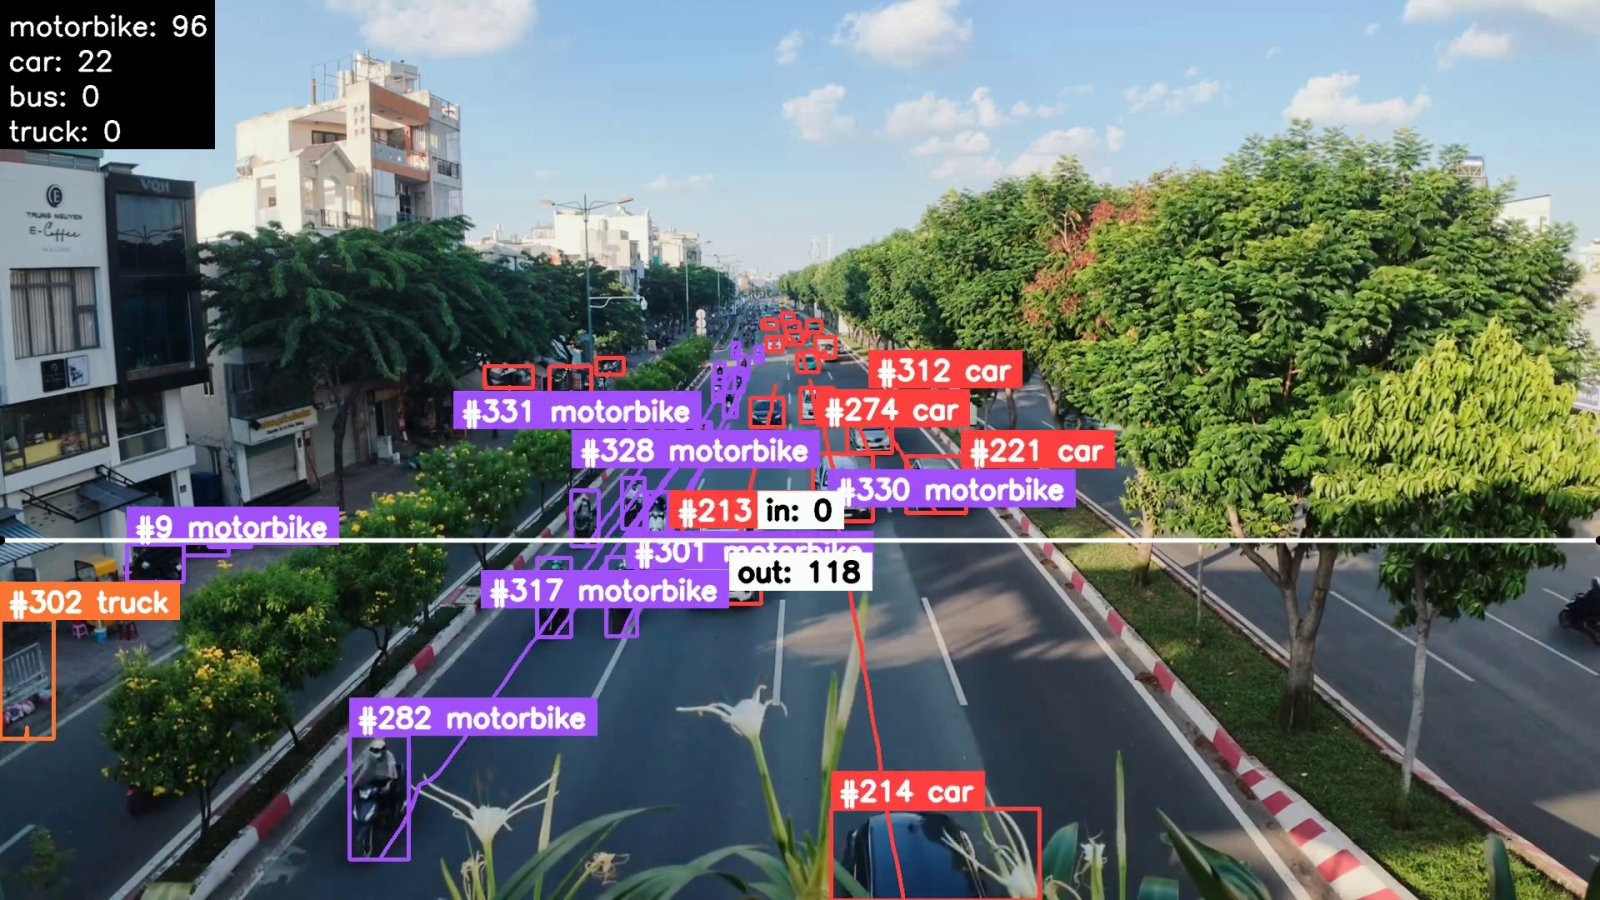
\includegraphics[width=\linewidth]{demo_pvd_goc_a.jpg}
  \caption{Một frame đầu ra của hệ thống trên clip đại lộ Phạm Văn Đồng (TP.HCM): box và nhãn ``\#ID lớp'' của từng
           xe, vết di chuyển, vạch đếm màu trắng và bảng đếm theo lớp ở góc trái (nguồn video: kênh YouTube Vietnam
           Naturally)}
  \label{fig:demo-pvd}
\end{figure}

\section{Ứng dụng của bài toán}

Hệ thống phát hiện, phân loại và theo dõi phương tiện là thành phần đầu vào của nhiều ứng dụng giao thông:
\begin{itemize}
  \item \textbf{Đếm lưu lượng.} Số xe qua một mặt cắt đường theo loại xe, theo hướng và theo thời gian. Đây là ứng dụng
        đề tài xây dựng và đánh giá sai số (mục~\ref{sec:dem-xe}).
  \item \textbf{Thống kê phục vụ quy hoạch và điều khiển tín hiệu.} Số liệu lưu lượng theo khung giờ giúp điều chỉnh
        chu kỳ đèn và đánh giá tải của nút giao.
  \item \textbf{Giám sát.} Quỹ đạo của từng xe là cơ sở để phát hiện các hành vi như đi ngược chiều hay dừng đỗ sai
        chỗ. Đề tài không làm các bài toán này nhưng đầu ra theo dõi có thể dùng lại cho chúng.
\end{itemize}

So với việc đếm thủ công hoặc dùng cảm biến đặt dưới mặt đường, cách làm dựa trên camera tận dụng được hạ tầng camera
có sẵn và cho biết thêm loại xe.

\section{Khó khăn và thách thức}
\label{sec:kho-khan}

Quá trình làm đề tài gặp sáu khó khăn chính; mỗi khó khăn dưới đây đi kèm số liệu đo được trong các chương sau.

\textbf{Thứ nhất, mật độ xe máy rất cao và che khuất lẫn nhau.} Tập test 30 frame cắt từ video ngã tư Hà Nội có 2.982
xe máy và 539 ô tô, tức khoảng 100 xe máy mỗi frame. Ở đèn đỏ, xe máy dừng sát nhau thành cụm, nhiều xe chỉ lộ ra một
phần. Đây là nơi mô hình bỏ sót nhiều nhất (Hình~\ref{fig:error-2}).

\textbf{Thứ hai, xe rất nhỏ ở xa.} Camera đặt cao nhìn dọc đại lộ thấy được cả đoạn đường dài, nên xe ở cuối đường chỉ
còn vài chục điểm ảnh. Trong tập test ban ngày \texttt{vn\_extra}, 52\% số xe có chiều cao dưới 32 điểm ảnh.

\textbf{Thứ ba, cảnh ban đêm.} Đèn pha và đèn hậu làm chói, thân xe tối màu lẫn vào nền, xe ở xa chỉ còn thấy đèn.
Mô hình dễ chỉ khoanh phần đèn sáng, hoặc nhầm xe máy chở hàng có đèn chói thành ô tô (mục~\ref{sec:phan-tich-loi}).

\textbf{Thứ tư, lệch miền dữ liệu.} Mô hình tốt trên tập test của bộ dữ liệu có sẵn chưa chắc tốt trên video mục tiêu.
Phiên bản v1 của đề tài đạt mAP50 0.861 trên tập test Roboflow nhưng trên frame Hà Nội AP50 của xe máy chỉ 0.045:
gần như không bắt được xe máy nhỏ của cảnh ngã tư.

\textbf{Thứ năm, thiếu dữ liệu đúng góc camera giao thông và định nghĩa lớp không thống nhất.} Các bộ dữ liệu có sẵn
phần lớn chụp ngang tầm mắt, từ drone hoặc từ một camera duy nhất. Mỗi bộ lại định nghĩa lớp theo cách riêng; ví dụ
xe van là \texttt{car} trong VisDrone nhưng là một lớp riêng trong KITTI và UA-DETRAC, còn xe Ford Transit 16 chỗ có
nơi xếp vào buýt, có nơi xếp vào ô tô.

\textbf{Thứ sáu, giới hạn tài nguyên.} Việc huấn luyện phụ thuộc hạn mức GPU của Kaggle; việc chạy demo diễn ra trên
laptop chỉ có CPU, nên mô hình phải đủ nhẹ. Mô hình chính xác nhất trong các thí nghiệm (RT-DETRv2-S) mất 1.53 giây
mỗi frame trên CPU, không dùng được cho video.

\section{Kết chương}

Chương này đã giới thiệu bài toán phát hiện, phân loại và theo dõi phương tiện từ video camera giao thông Việt Nam,
gồm ba bài toán con và ứng dụng đếm xe qua vạch. Các khó khăn chính là mật độ xe máy cao, xe nhỏ ở xa, cảnh đêm, lệch
miền dữ liệu, thiếu dữ liệu đúng góc camera và giới hạn phần cứng. Chương~\ref{chap:lythuyet} trình bày cơ sở lý
thuyết của các mô hình và chỉ số được dùng để giải quyết bài toán.

\chapter{CƠ SỞ LÝ THUYẾT}
\label{chap:lythuyet}

Chương này trình bày nền tảng của các thành phần trong hệ thống: mạng nơ-ron tích chập và bài toán phát hiện đối
tượng, hai họ mô hình phát hiện được so sánh (YOLO và DETR), các thuật toán theo dõi đa đối tượng họ SORT, và các chỉ
số đánh giá.

\section{Mạng nơ-ron tích chập và bài toán phát hiện đối tượng}

\subsection{Mạng nơ-ron tích chập}

Mạng nơ-ron tích chập (CNN) xử lý ảnh bằng các lớp tích chập: mỗi lớp trượt một tập bộ lọc nhỏ trên bản đồ đặc trưng
đầu vào. Với đầu vào $X$ có $C$ kênh, bộ lọc kích thước $k \times k$ và bước trượt $s$, kênh thứ $c'$ của đầu ra là
\begin{equation}
  Y(i, j, c') = \sum_{c=1}^{C} \sum_{u=0}^{k-1} \sum_{v=0}^{k-1} W(u, v, c, c')\, X(i s + u,\; j s + v,\; c) + b_{c'}
  \label{eq:conv}
\end{equation}
Công thức (\ref{eq:conv}): phép tích chập hai chiều.

Với:
\begin{itemize}
  \item $W$: trọng số bộ lọc, dùng chung cho mọi vị trí trong ảnh;
  \item $b_{c'}$: độ lệch của kênh đầu ra $c'$;
  \item $s$: bước trượt; $s = 2$ làm bản đồ đặc trưng nhỏ đi một nửa mỗi chiều.
\end{itemize}

Vì trọng số dùng chung theo vị trí, số tham số không phụ thuộc kích thước ảnh và mạng nhận ra cùng một mẫu (bánh xe,
kính chắn gió) ở mọi chỗ trong ảnh. Xếp chồng nhiều lớp tích chập, chuẩn hoá theo batch và hàm kích hoạt phi tuyến (các
mô hình YOLO gần đây dùng SiLU, $\mathrm{SiLU}(x) = x \cdot \sigma(x)$) giúp vùng nhìn (receptive field) của mỗi nơ-ron
lớn dần: lớp nông bắt cạnh và góc, lớp sâu bắt hình dạng cả chiếc xe. Mạng ResNet~\cite{he2016resnet} thêm kết nối tắt
$y = F(x) + x$ để huấn luyện được mạng sâu; RT-DETRv2-S dùng ResNet-18 làm phần trích đặc trưng.

\subsection{Bài toán phát hiện đối tượng}

Mô hình phát hiện nhận một ảnh và trả về tập dự đoán $\{(b_k, c_k, s_k)\}$, trong đó $b_k = (x, y, w, h)$ là box (toạ độ
tâm, chiều rộng, chiều cao), $c_k$ là lớp và $s_k$ là điểm tin cậy. Các mô hình hiện đại thường gồm ba phần:
\begin{itemize}
  \item \textbf{Backbone}: mạng trích đặc trưng, cho ra các bản đồ đặc trưng ở nhiều độ phân giải (thường là 1/8, 1/16 và
        1/32 ảnh gốc);
  \item \textbf{Neck}: trộn đặc trưng giữa các mức để mức độ phân giải cao (dành cho vật nhỏ) cũng mang thông tin ngữ
        nghĩa của mức sâu;
  \item \textbf{Head}: dự đoán box và lớp tại từng vị trí trên các bản đồ đặc trưng.
\end{itemize}

Mức độ trùng khớp giữa hai box $A$ và $B$ được đo bằng tỉ lệ giao trên hợp (IoU):
\begin{equation}
  \mathrm{IoU}(A, B) = \frac{|A \cap B|}{|A \cup B|}
  \label{eq:iou}
\end{equation}
Công thức (\ref{eq:iou}): tỉ lệ giao trên hợp của hai box, nhận giá trị từ 0 (không giao nhau) đến 1 (trùng khít).

IoU được dùng ở ba chỗ: khi gán nhãn huấn luyện (dự đoán nào chịu trách nhiệm cho xe nào), khi chấm điểm (một dự đoán
là đúng nếu IoU với box nhãn vượt ngưỡng) và khi theo dõi (ghép box giữa hai frame).

Nhiều mô hình phát hiện, kể cả các bản YOLO trước YOLOv10, cho ra nhiều box chồng lên cùng một xe. Bước hậu xử lý
\emph{loại bỏ không cực đại} (NMS) giữ box có điểm cao nhất rồi xoá các box khác có IoU với nó vượt ngưỡng. NMS có
một tham số phải chỉnh tay và hoạt động kém ở cảnh xe đứng sát nhau: hai xe máy dừng cạnh nhau có IoU cao, NMS có thể
xoá nhầm một xe. Cả YOLO26 và họ DETR dùng trong đề tài đều không cần NMS.

\section{Họ mô hình YOLO và YOLO26}

\subsection{Ý tưởng phát hiện một giai đoạn}

YOLO~\cite{redmon2016yolo} coi phát hiện đối tượng là một bài toán hồi quy: một lần truyền xuôi qua mạng cho ra trực
tiếp toạ độ box và xác suất lớp tại mọi vị trí, thay cho cách hai giai đoạn (đề xuất vùng rồi phân loại từng vùng). Cách
làm này nhanh, phù hợp xử lý video. Các phiên bản sau giữ ý tưởng đó và cải tiến dần backbone, neck đa tỉ lệ, cách gán
nhãn và hàm mất mát.

\subsection{YOLO26}

YOLO26~\cite{jocher2026yolo26} là thế hệ YOLO mới nhất của Ultralytics~\cite{ultralytics}, có năm cỡ n, s, m, l, x. Đề
tài dùng cỡ n (2.5 triệu tham số) làm mô hình triển khai và cỡ s (10.0 triệu tham số) để so sánh. Các điểm khác biệt
chính so với thế hệ trước:
\begin{itemize}
  \item \textbf{Phát hiện đầu cuối, không cần NMS.} Theo hướng của YOLOv10~\cite{wang2024yolov10}, khi suy luận mô hình
        dùng đầu ra gán nhãn một-một: mỗi xe chỉ ứng với một dự đoán, nên đầu ra dùng được ngay, không qua NMS.
  \item \textbf{Bỏ Distribution Focal Loss (DFL).} Box được hồi quy trực tiếp, giúp mô hình gọn hơn khi xuất sang các
        định dạng triển khai như OpenVINO.
  \item \textbf{ProgLoss và STAL.} ProgLoss cân bằng dần các thành phần mất mát trong quá trình huấn luyện; STAL là cách
        gán nhãn chú ý tới vật nhỏ. Cả hai nhắm vào vật nhỏ, đúng với xe máy ở xa trong bài toán này.
  \item \textbf{Optimizer MuSGD}, kết hợp SGD với Muon, dùng cho các lần huấn luyện dài.
\end{itemize}

Nhật ký huấn luyện của đề tài ghi ba thành phần mất mát: mất mát box dựa trên IoU, mất mát phân lớp và mất mát L1 trên
toạ độ box. Mất mát phân lớp là entropy chéo nhị phân (BCE) tính riêng cho từng lớp:
\begin{equation}
  \mathcal{L}_{\mathrm{cls}} = -\frac{1}{N} \sum_{i=1}^{N} \sum_{c=1}^{K}
  \Big[ y_{ic} \log p_{ic} + (1 - y_{ic}) \log (1 - p_{ic}) \Big]
  \label{eq:bce}
\end{equation}
Công thức (\ref{eq:bce}): mất mát phân lớp entropy chéo nhị phân.

Với:
\begin{itemize}
  \item $N$: số dự đoán được tính mất mát; $K = 4$: số lớp;
  \item $y_{ic}$: nhãn đích của dự đoán $i$ với lớp $c$;
  \item $p_{ic}$: xác suất mô hình dự đoán (sau hàm sigmoid).
\end{itemize}

Tổng mất mát là tổng có trọng số $\mathcal{L} = \lambda_{\mathrm{box}} \mathcal{L}_{\mathrm{box}} +
\lambda_{\mathrm{cls}} \mathcal{L}_{\mathrm{cls}} + \lambda_{L1} \mathcal{L}_{L1}$, với các hệ số lấy theo mặc định
của thư viện.

\textbf{Ưu điểm:} nhanh, nhẹ, có sẵn công cụ huấn luyện, xuất mô hình và theo dõi đối tượng trong cùng thư viện;
không cần NMS. \textbf{Nhược điểm:} ảnh được thu nhỏ về 960 điểm ảnh cạnh dài (với cấu hình của đề tài), nên xe rất
nhỏ ở xa mất chi tiết; cỡ n có ít tham số nên kém hơn cỡ lớn ở cảnh khó.

\section{Transformer và họ mô hình DETR}

\subsection{Cơ chế attention}

Transformer~\cite{vaswani2017attention} xây dựng trên cơ chế attention: mỗi phần tử của chuỗi đầu vào tổng hợp thông
tin từ mọi phần tử khác theo trọng số học được.
\begin{equation}
  \mathrm{Attention}(Q, K, V) = \mathrm{softmax}\!\left( \frac{Q K^{\top}}{\sqrt{d_k}} \right) V
  \label{eq:attention}
\end{equation}
Công thức (\ref{eq:attention}): attention tích vô hướng có chuẩn hoá.

Với:
\begin{itemize}
  \item $Q$, $K$, $V$: ma trận truy vấn (query), khoá (key) và giá trị (value), là các phép chiếu tuyến tính của đầu
        vào;
  \item $d_k$: số chiều của khoá; chia cho $\sqrt{d_k}$ để hàm softmax không bị bão hoà.
\end{itemize}

Attention nhiều đầu (multi-head) chạy song song nhiều phép attention với các phép chiếu khác nhau rồi ghép kết quả.
Khác với tích chập chỉ nhìn một vùng lân cận, attention nhìn toàn ảnh, nhưng chi phí tăng theo bình phương số phần tử.

\subsection{DETR: phát hiện như bài toán dự đoán tập hợp}

DETR~\cite{carion2020detr} dùng CNN trích đặc trưng, đưa qua bộ mã hoá và bộ giải mã Transformer với $N$ truy vấn đối
tượng (object query); mỗi truy vấn cho ra một box và một lớp, có thể là lớp ``không có đối tượng'' ($\varnothing$).
Khi huấn luyện, $N$ dự đoán được ghép một-một với các box nhãn bằng thuật toán Hungarian:
\begin{equation}
  \begin{split}
    \hat{\sigma} &= \arg\min_{\sigma} \sum_{i=1}^{N} \mathcal{L}_{\mathrm{match}}\big(y_i, \hat{y}_{\sigma(i)}\big) \\
    \mathcal{L}_{\mathrm{match}} &= -\mathbf{1}_{\{c_i \neq \varnothing\}}\, \hat{p}_{\sigma(i)}(c_i)
      + \mathbf{1}_{\{c_i \neq \varnothing\}}\, \mathcal{L}_{\mathrm{box}}\big(b_i, \hat{b}_{\sigma(i)}\big)
  \end{split}
  \label{eq:detr-match}
\end{equation}
Công thức (\ref{eq:detr-match}): ghép cặp tối ưu giữa nhãn và dự đoán trong DETR.

Với:
\begin{itemize}
  \item $\sigma$: một hoán vị gán mỗi nhãn $y_i = (c_i, b_i)$ cho một dự đoán $\hat{y}_{\sigma(i)}$;
  \item $\hat{p}_{\sigma(i)}(c_i)$: xác suất dự đoán $\sigma(i)$ gán cho lớp đúng $c_i$;
  \item $\mathcal{L}_{\mathrm{box}} = \lambda_{L1} \lVert b_i - \hat{b}_{\sigma(i)} \rVert_1 +
        \lambda_{\mathrm{giou}} \mathcal{L}_{\mathrm{giou}}$: mất mát box.
\end{itemize}

Thành phần GIoU khắc phục việc IoU bằng 0 cho mọi cặp box không giao nhau:
\begin{equation}
  \mathrm{GIoU}(A, B) = \mathrm{IoU}(A, B) - \frac{|C| - |A \cup B|}{|C|},
  \qquad \mathcal{L}_{\mathrm{giou}} = 1 - \mathrm{GIoU}
  \label{eq:giou}
\end{equation}
Công thức (\ref{eq:giou}): IoU tổng quát, với $C$ là box nhỏ nhất bao cả $A$ và $B$.

Vì ghép một-một, mỗi xe chỉ ứng với một dự đoán và DETR không cần NMS. Nhược điểm của DETR gốc là hội tụ chậm (hàng
trăm epoch trên COCO) và chậm khi suy luận.

\subsection{RT-DETR và RT-DETRv2}

RT-DETR~\cite{zhao2024rtdetr} đưa họ DETR về tốc độ thời gian thực trên GPU nhờ ba thay đổi:
\begin{itemize}
  \item \textbf{Bộ mã hoá lai.} Attention trong cùng một mức (AIFI) chỉ chạy trên bản đồ đặc trưng sâu nhất (1/32),
        nơi số phần tử ít; việc trộn đặc trưng giữa các mức (CCFM) làm bằng tích chập.
  \item \textbf{Chọn truy vấn theo IoU.} Truy vấn khởi tạo cho bộ giải mã được chọn từ các vị trí có điểm phân lớp và
        IoU dự kiến cao, thay cho truy vấn học tự do.
  \item \textbf{Attention biến dạng trong bộ giải mã.} Mỗi truy vấn chỉ lấy mẫu một số ít điểm quanh điểm tham chiếu:
\end{itemize}
\begin{equation}
  \mathrm{DeformAttn}(z_q, p_q, x) = \sum_{m=1}^{M} W_m \Big[ \sum_{k=1}^{K} A_{mqk} \cdot W'_m\, x\big(p_q +
  \Delta p_{mqk}\big) \Big]
  \label{eq:deform}
\end{equation}
Công thức (\ref{eq:deform}): attention biến dạng.

Với:
\begin{itemize}
  \item $z_q$, $p_q$: đặc trưng và điểm tham chiếu của truy vấn $q$;
  \item $M$: số đầu attention; $K$: số điểm lấy mẫu mỗi đầu;
  \item $\Delta p_{mqk}$: độ lệch vị trí học được; $A_{mqk}$: trọng số attention, tổng theo $k$ bằng 1.
\end{itemize}

Mất mát phân lớp của RT-DETR là Varifocal Loss (VFL), dùng IoU giữa box dự đoán và box nhãn làm nhãn mềm $q$:
\begin{equation}
  \mathrm{VFL}(p, q) =
  \begin{cases}
    -q \big( q \log p + (1 - q) \log (1 - p) \big), & q > 0 \\
    -\alpha\, p^{\gamma} \log (1 - p), & q = 0
  \end{cases}
  \label{eq:vfl}
\end{equation}
Công thức (\ref{eq:vfl}): Varifocal Loss, với $p$ là điểm dự đoán, $\alpha$ và $\gamma$ là hệ số giảm trọng số cho
mẫu nền.

RT-DETRv2~\cite{lv2024rtdetrv2} giữ kiến trúc trên và thêm một số cải tiến không làm chậm suy luận (bag-of-freebies):
số điểm lấy mẫu khác nhau cho từng mức đặc trưng, toán tử lấy mẫu rời rạc thuận tiện khi triển khai, tăng cường dữ
liệu động và siêu tham số điều chỉnh theo cỡ mô hình. Khi huấn luyện còn dùng thêm truy vấn nhiễu (denoising) để bộ giải
mã hội tụ nhanh hơn. Bản RT-DETRv2-S dùng backbone ResNet-18 và có 20.1 triệu tham số.

\textbf{Ưu điểm:} box khít, không cần NMS, nhìn được ngữ cảnh toàn ảnh. \textbf{Nhược điểm:} nặng hơn YOLO cùng thế
hệ; trên CPU chậm hơn nhiều lần (mục~\ref{sec:toc-do}).

\section{Theo dõi đa đối tượng}

\subsection{Theo dõi dựa trên phát hiện}

Các thuật toán theo dõi trong đề tài đều theo vòng lặp sau cho mỗi frame $t$:
\begin{enumerate}
  \item chạy mô hình phát hiện, được tập box $D_t$;
  \item dự đoán vị trí ở frame $t$ của mọi quỹ đạo (track) đang theo dõi bằng bộ lọc Kalman;
  \item ghép box $D_t$ với các track dựa trên IoU giữa box và vị trí dự đoán;
  \item cập nhật track được ghép, tạo track mới cho box chưa ghép đủ tin cậy, giữ track chưa ghép ở trạng thái ``mất''
        thêm một số frame trước khi xoá.
\end{enumerate}

\subsection{Bộ lọc Kalman}

Bộ lọc Kalman~\cite{kalman1960} ước lượng trạng thái của từng xe dưới giả thiết vận tốc không đổi. Với BoT-SORT, trạng
thái là $\mathbf{x} = [x_c, y_c, w, h, \dot{x}_c, \dot{y}_c, \dot{w}, \dot{h}]^{\top}$ (tâm, kích thước box và vận tốc
của chúng). Mỗi frame gồm hai bước:
\begin{equation}
  \hat{\mathbf{x}}_{t|t-1} = F \hat{\mathbf{x}}_{t-1}, \qquad P_{t|t-1} = F P_{t-1} F^{\top} + Q
  \label{eq:kalman-predict}
\end{equation}
Công thức (\ref{eq:kalman-predict}): bước dự đoán.
\begin{equation}
  \begin{split}
    K_t &= P_{t|t-1} H^{\top} \big( H P_{t|t-1} H^{\top} + R \big)^{-1} \\
    \hat{\mathbf{x}}_{t} &= \hat{\mathbf{x}}_{t|t-1} + K_t \big( \mathbf{z}_t - H \hat{\mathbf{x}}_{t|t-1} \big) \\
    P_t &= (I - K_t H) P_{t|t-1}
  \end{split}
  \label{eq:kalman-update}
\end{equation}
Công thức (\ref{eq:kalman-update}): bước cập nhật khi track được ghép với một box.

Với:
\begin{itemize}
  \item $F$: ma trận chuyển trạng thái (vị trí cộng vận tốc); $H$: ma trận quan sát, lấy 4 thành phần box từ trạng thái;
  \item $P$: hiệp phương sai của ước lượng; $Q$, $R$: nhiễu của mô hình chuyển động và nhiễu đo;
  \item $\mathbf{z}_t$: box được ghép ở frame $t$; $K_t$: hệ số Kalman, cân bằng giữa dự đoán và quan sát.
\end{itemize}

Khi xe bị che vài frame, track không được cập nhật nhưng bước dự đoán vẫn đẩy vị trí theo vận tốc, nên khi xe xuất hiện
lại vẫn có thể ghép đúng.

\subsection{Ghép cặp bằng thuật toán Hungarian}

Giữa $n$ track và $m$ box, ma trận chi phí có phần tử $c_{ij} = 1 - \mathrm{IoU}(\hat{b}_i, d_j)$. Thuật toán
Hungarian~\cite{kuhn1955hungarian} tìm phép gán một-một có tổng chi phí nhỏ nhất:
\begin{equation}
  \min_{x_{ij} \in \{0, 1\}} \sum_{i=1}^{n} \sum_{j=1}^{m} c_{ij} x_{ij}
  \quad \text{sao cho} \quad \sum_{j} x_{ij} \le 1,\; \sum_{i} x_{ij} \le 1
  \label{eq:hungarian}
\end{equation}
Công thức (\ref{eq:hungarian}): bài toán gán. Các cặp có chi phí vượt ngưỡng ghép bị loại dù được thuật toán chọn.

\subsection{Các thuật toán theo dõi họ SORT}

\textbf{SORT}~\cite{bewley2016sort} là dạng cơ bản: Kalman để dự đoán, Hungarian theo IoU để ghép. Track mới chỉ được
xác nhận sau vài frame liên tiếp có box (\texttt{min\_hits}) và bị xoá sau một số frame không được ghép.

\textbf{ByteTrack}~\cite{zhang2022bytetrack} giữ lại cả box điểm thấp. Box được chia hai nhóm theo điểm tin cậy: lần
ghép thứ nhất chỉ dùng box điểm cao; các track còn lại được ghép lần hai với box điểm thấp. Xe bị che một phần thường
có điểm thấp, nên lần ghép thứ hai giúp track không bị đứt. Chỉ box điểm cao chưa ghép mới tạo track mới. Vì lý do
này, ngưỡng tin cậy của mô hình phát hiện trong hệ thống được đặt ở 0.1 thay cho 0.25 thông thường: các box từ 0.1 đến
0.25 không tạo track mới nhưng được dùng ở lần ghép thứ hai.

\textbf{BoT-SORT}~\cite{aharon2022botsort} dựa trên ByteTrack và thêm ba cải tiến: trạng thái Kalman dùng trực tiếp
chiều rộng và chiều cao box; bù chuyển động camera (GMC) bằng cách ước lượng phép biến đổi giữa hai frame từ luồng
quang học thưa rồi áp vào vị trí dự đoán; và tuỳ chọn kết hợp đặc trưng ngoại hình (ReID) với IoU khi ghép.

\textbf{OC-SORT}~\cite{cao2023ocsort} xử lý trường hợp xe bị che lâu: khi track được ghép lại sau thời gian mất, thuật
toán dựng lại quỹ đạo ảo từ quan sát cuối để sửa sai số tích luỹ của Kalman, và dùng hướng chuyển động thực tế làm
thêm một thành phần chi phí khi ghép.

\section{Các chỉ số đánh giá}
\label{sec:chi-so}

\subsection{Chỉ số phát hiện: Precision, Recall, AP và mAP}

Một dự đoán là đúng (TP) nếu cùng lớp và có IoU với một box nhãn chưa được ghép vượt ngưỡng; các dự đoán được xét lần
lượt theo điểm tin cậy giảm dần. Dự đoán không ghép được là phát hiện thừa (FP), box nhãn không được ghép là bỏ sót (FN).
\begin{equation}
  \mathrm{Precision} = \frac{TP}{TP + FP}, \qquad \mathrm{Recall} = \frac{TP}{TP + FN}
  \label{eq:pr}
\end{equation}
Công thức (\ref{eq:pr}): độ chính xác và độ bao phủ.

Quét ngưỡng tin cậy từ cao xuống thấp cho đường cong Precision–Recall. Độ chính xác trung bình (AP) theo quy ước
COCO~\cite{lin2014coco} là trung bình độ chính xác nội suy tại 101 mức recall:
\begin{equation}
  \mathrm{AP} = \frac{1}{101} \sum_{r \in \{0, 0.01, \ldots, 1\}} p_{\mathrm{interp}}(r), \qquad
  p_{\mathrm{interp}}(r) = \max_{\tilde{r} \ge r} p(\tilde{r})
  \label{eq:ap}
\end{equation}
Công thức (\ref{eq:ap}): AP nội suy 101 điểm của COCO.

mAP là trung bình AP trên các lớp. mAP50 tính ở ngưỡng IoU 0.5; mAP50-95 lấy trung bình thêm trên 10 ngưỡng IoU 0.50,
0.55, \ldots, 0.95, nên đòi hỏi box khít hơn. Trong đề tài, \textbf{mAP50 chính} là trung bình AP50 của xe máy và ô tô:
các tập test Việt Nam có rất ít xe buýt và xe tải (tập test Hà Nội chỉ có 5 xe buýt và 2 xe tải), AP của hai lớp này
nhảy giữa 0 và 1 theo từng box nên không đưa vào chỉ số chính.

Một số vùng trong ảnh có xe nhưng không thể gán nhãn rõ ràng (xe bị cây che gần hết, cụm xe quá xa). Theo quy ước vùng
bỏ qua của KITTI~\cite{geiger2012kitti} (\texttt{DontCare}) và COCO (\texttt{iscrowd}), các vùng này được gán lớp
\texttt{ignore}: dự đoán rơi vào vùng ignore không bị tính là thừa, và xe trong vùng không bị tính là bỏ sót.

\subsection{MOTA}

MOTA~\cite{bernardin2008clear} gộp ba loại lỗi trên toàn bộ video:
\begin{equation}
  \mathrm{MOTA} = 1 - \frac{\sum_{t} \big( \mathrm{FN}_t + \mathrm{FP}_t + \mathrm{IDSW}_t \big)}{\sum_{t} \mathrm{GT}_t}
  \label{eq:mota}
\end{equation}
Công thức (\ref{eq:mota}): độ chính xác theo dõi đa đối tượng.

Với:
\begin{itemize}
  \item $\mathrm{FN}_t$, $\mathrm{FP}_t$: số box bỏ sót và thừa ở frame $t$;
  \item $\mathrm{IDSW}_t$: số lần một xe bị đổi ID so với frame trước;
  \item $\mathrm{GT}_t$: số box nhãn ở frame $t$.
\end{itemize}

MOTA bị chi phối bởi FN và FP, tức chủ yếu đo chất lượng phát hiện; số lần đổi ID thường nhỏ so với hai thành phần kia.

\subsection{IDF1}

IDF1~\cite{ristani2016idf1} đo mức giữ đúng danh tính. Toàn bộ quỹ đạo nhãn và quỹ đạo dự đoán được ghép một-một sao
cho số frame trùng khớp lớn nhất; IDTP là số box thuộc cặp quỹ đạo được ghép và trùng khớp, IDFP và IDFN là phần còn lại.
\begin{equation}
  \begin{gathered}
    \mathrm{IDF1} = \frac{2\,\mathrm{IDTP}}{2\,\mathrm{IDTP} + \mathrm{IDFP} + \mathrm{IDFN}} \\
    \mathrm{IDP} = \frac{\mathrm{IDTP}}{\mathrm{IDTP} + \mathrm{IDFP}}, \qquad
    \mathrm{IDR} = \frac{\mathrm{IDTP}}{\mathrm{IDTP} + \mathrm{IDFN}}
  \end{gathered}
  \label{eq:idf1}
\end{equation}
Công thức (\ref{eq:idf1}): IDF1, độ chính xác danh tính IDP và độ bao phủ danh tính IDR.

IDR chỉ phụ thuộc vào quỹ đạo nhãn được theo đúng bao nhiêu, không bị phạt khi hệ thống phát hiện thêm xe không có
nhãn. Tính chất này được dùng khi đánh giá trên tập VnTraffic có nhãn thiếu (mục~\ref{sec:theo-doi}).

\subsection{HOTA}

HOTA~\cite{luiten2021hota} tách đánh giá thành hai phần, phát hiện (DetA) và liên kết (AssA), rồi lấy trung bình nhân.
Tại ngưỡng IoU $\alpha$, sau khi ghép box nhãn với box dự đoán:
\begin{equation}
  \begin{gathered}
    \mathrm{DetA}_{\alpha} = \frac{|TP|}{|TP| + |FN| + |FP|} \\
    \mathrm{AssA}_{\alpha} = \frac{1}{|TP|} \sum_{c \in TP} \frac{|TPA(c)|}{|TPA(c)| + |FNA(c)| + |FPA(c)|}
  \end{gathered}
  \label{eq:deta-assa}
\end{equation}
\begin{equation}
  \mathrm{HOTA}_{\alpha} = \sqrt{\mathrm{DetA}_{\alpha} \cdot \mathrm{AssA}_{\alpha}}, \qquad
  \mathrm{HOTA} = \frac{1}{19} \sum_{\alpha \in \{0.05, 0.10, \ldots, 0.95\}} \mathrm{HOTA}_{\alpha}
  \label{eq:hota}
\end{equation}
Công thức (\ref{eq:deta-assa}) và (\ref{eq:hota}): các thành phần của HOTA.

Với:
\begin{itemize}
  \item $TPA(c)$: tập các cặp TP có cùng ID nhãn và cùng ID dự đoán với cặp $c$, tức những frame quỹ đạo được nối đúng;
  \item $FNA(c)$, $FPA(c)$: các box của cùng xe nhãn (hoặc cùng track dự đoán) với $c$ nhưng không được ghép với nhau.
\end{itemize}

Nhờ tách hai thành phần, HOTA cho biết điểm thấp là do phát hiện kém hay do nối quỹ đạo kém. Đề tài tính MOTA, IDF1
và HOTA bằng TrackEval~\cite{trackeval}, bộ chấm được dùng cho benchmark MOTChallenge~\cite{milan2016mot16}.

\subsection{Khoảng tin cậy bootstrap}
\label{sec:bootstrap}

Các tập test của đề tài nhỏ, nên một chênh lệch mAP nhỏ có thể chỉ do mẫu ảnh. Để biết chênh lệch có đáng tin không,
đề tài lấy mẫu lại có hoàn lại các ảnh của tập test 1.000 lần, tính lại mAP trên mỗi mẫu, rồi lấy phân vị 2.5\% và
97.5\% làm khoảng tin cậy 95\%~\cite{efron1993bootstrap}. Cần khoảng 1.000 lần trở lên thì hai phân vị này mới ổn định;
với vài chục lần, chúng gần như chỉ là giá trị nhỏ nhất và lớn nhất của các mẫu. Việc ghép dự đoán với nhãn được làm
một lần cho từng ảnh, mỗi lần lấy mẫu chỉ gộp lại kết quả đã ghép của các ảnh được chọn rồi tính AP theo đúng công thức
(\ref{eq:ap}), nên 1.000 lần vẫn nhanh. Hai mô hình có khoảng tin cậy chồng nhau được coi là chưa phân biệt được.

Lấy mẫu lại từng ảnh là coi các ảnh độc lập với nhau. Với frame cắt từ cùng một clip thì không đúng: hai frame cách nhau
vài giây chứa phần lớn là cùng những chiếc xe, nên tập 30 frame chứa ít thông tin hơn 30 ảnh độc lập và khoảng tin cậy
tính theo ảnh hẹp hơn thực tế. Cách chuẩn cho dữ liệu có tương quan là lấy mẫu lại theo khối~\cite{kunsch1989block}
hoặc theo cụm~\cite{field2007cluster}: chia ảnh thành các nhóm gần như độc lập với nhau rồi lấy mẫu lại cả nhóm. Đề tài
dùng thêm cách này cho mọi tập frame cắt từ video, với nhóm là các khối 10 giây liên tiếp trong cùng một clip. Độ dài khối
được chọn từ nhãn tracking của clip Phạm Văn Đồng: 90\% số xe ở trong khung hình dưới 8.2 giây (trung vị 1.3 giây),
nên hai khối cách nhau hơn 10 giây hầu như không chung chiếc xe nào. Với UA-DETRAC, mỗi video là một nhóm. Tập có dưới 5
nhóm thì không tính khoảng tin cậy theo khối, vì khi đó số cách lấy mẫu lại khác nhau quá ít.

Cả hai cách đều chỉ đo dao động do mẫu ảnh test, không đo dao động giữa các lần huấn luyện.

\section{Kết luận chương}

Chương này đã trình bày cơ sở của hai họ mô hình phát hiện được dùng trong đề tài: YOLO26 thuộc họ CNN, phát hiện đầu
cuối không cần NMS, và RT-DETRv2 thuộc họ Transformer, ghép cặp Hungarian khi huấn luyện. Phần theo dõi gồm bộ lọc
Kalman, thuật toán Hungarian và các biến thể SORT, ByteTrack, BoT-SORT, OC-SORT. Các chỉ số mAP, MOTA, IDF1 và HOTA đo
lần lượt chất lượng phát hiện, độ chính xác theo dõi tổng thể, khả năng giữ danh tính và sự cân bằng giữa phát hiện
với liên kết. Chương~\ref{chap:xaydung} mô tả cách các thành phần này được ghép thành hệ thống và huấn luyện trên dữ
liệu Việt Nam.

\chapter{XÂY DỰNG HỆ THỐNG}
\label{chap:xaydung}

Chương này mô tả cách xây dựng hệ thống: thu thập và chia dữ liệu, gán nhãn, huấn luyện mô hình phát hiện, giao thức
so sánh hai họ kiến trúc, chọn thuật toán theo dõi và ghép các thành phần thành pipeline đếm xe. Toàn bộ mã nguồn viết
bằng Python, dùng các thư viện Ultralytics~\cite{ultralytics} (huấn luyện và theo dõi), Supervision~\cite{supervision}
(đếm qua vạch, vẽ kết quả), Transformers~\cite{transformers} (RT-DETRv2) và TrackEval~\cite{trackeval} (chấm theo dõi).

\section{Dữ liệu}

\subsection{Nguồn dữ liệu huấn luyện}

Không có bộ dữ liệu công khai nào khớp hoàn toàn với bài toán, nên đề tài gộp bảy nguồn, mỗi nguồn bù một điểm thiếu
của các nguồn còn lại (Bảng~\ref{tab:nguon-du-lieu}, Hình~\ref{fig:nguon-du-lieu}). Nhãn của mọi nguồn được đổi về
bốn lớp của đề tài theo tên lớp; riêng xe van trong VisDrone được gộp vào ô tô.

\begin{table}[H]
  \centering
  \caption{Các nguồn dữ liệu huấn luyện}
  \label{tab:nguon-du-lieu}
  \small
  \begin{tabularx}{\linewidth}{|p{3.3cm}|L|p{2.3cm}|p{2.1cm}|}
    \hline
    \thead{Nguồn} & \thead{Đặc điểm và cách dùng} & \thead{Dùng cho} & \thead{Giấy phép} \\ \hline
    vietnamese-vehicle v3~\cite{roboflow_vnvehicle} & Ảnh xe Việt Nam từ nhiều cảnh; nguồn duy nhất được chia ra cả
      val và test & Train, val, test & CC BY 4.0 \\ \hline
    vehicle-vietnam-cantho v19~\cite{roboflow_cantho} & Gần như một camera cố định ở Cần Thơ; lấy 300 ảnh & Train &
      CC BY 4.0 \\ \hline
    vehicle-detection v2~\cite{roboflow_indo} & Gần như một camera cố định; lấy 300 ảnh & Train & CC BY 4.0 \\ \hline
    VisDrone2019-DET~\cite{zhu2022visdrone} & Ảnh từ drone, rất nhiều xe máy nhỏ; chỉ lấy 909 ảnh có từ 10 xe máy trở
      lên & Train & Chỉ dùng cho nghiên cứu \\ \hline
    UVH-26~\cite{sharma2025uvh26} & Ảnh camera giao thông Bengaluru (Ấn Độ), khoảng 2.800 camera; lấy 2.000 ảnh,
      đổi 14 lớp về 4 lớp & Train & CC BY 4.0 \\ \hline
    Video ngã tư Hà Nội (YouTube, kênh Raw Street Capture 101) & 69 frame nhãn tự động (lặp 4 lần khi train) và 10
      frame val nhãn tay; 30 frame khác làm test & Train, val, test & Chỉ dùng học tập \\ \hline
    Video đường phố TP.HCM ban đêm (YouTube, kênh Midnight Soundscape) & 288 frame từ hai camera, nhãn tự động; chỉ
      có từ v6 & Train & Chỉ dùng học tập \\ \hline
  \end{tabularx}
\end{table}

\begin{figure}[H]
  \centering
  \begin{subfigure}{0.32\linewidth}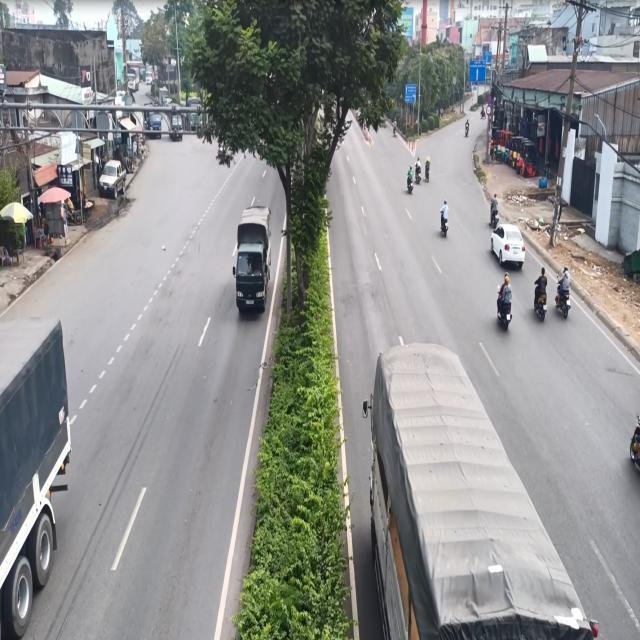
\includegraphics[width=\linewidth]{data_vnvehicle.jpg}\caption{vietnamese-vehicle}\end{subfigure}\hfill
  \begin{subfigure}{0.32\linewidth}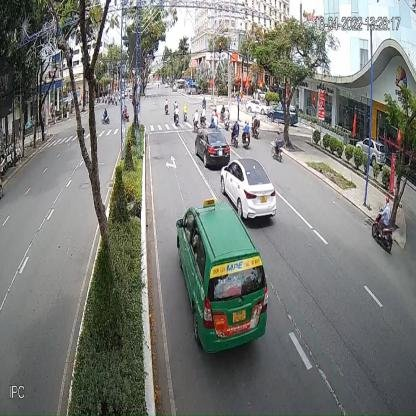
\includegraphics[width=\linewidth]{data_cantho.jpg}\caption{vehicle-vietnam-cantho}\end{subfigure}\hfill
  \begin{subfigure}{0.32\linewidth}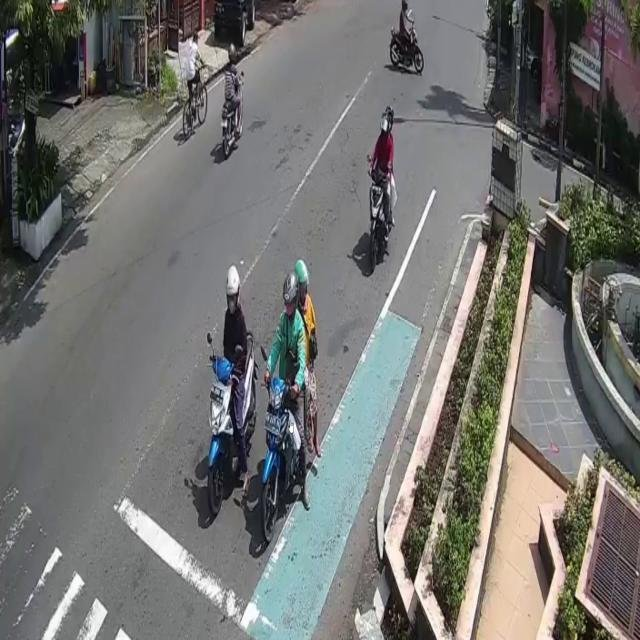
\includegraphics[width=\linewidth]{data_indo.jpg}\caption{vehicle-detection}\end{subfigure}\\[4pt]
  \begin{subfigure}{0.32\linewidth}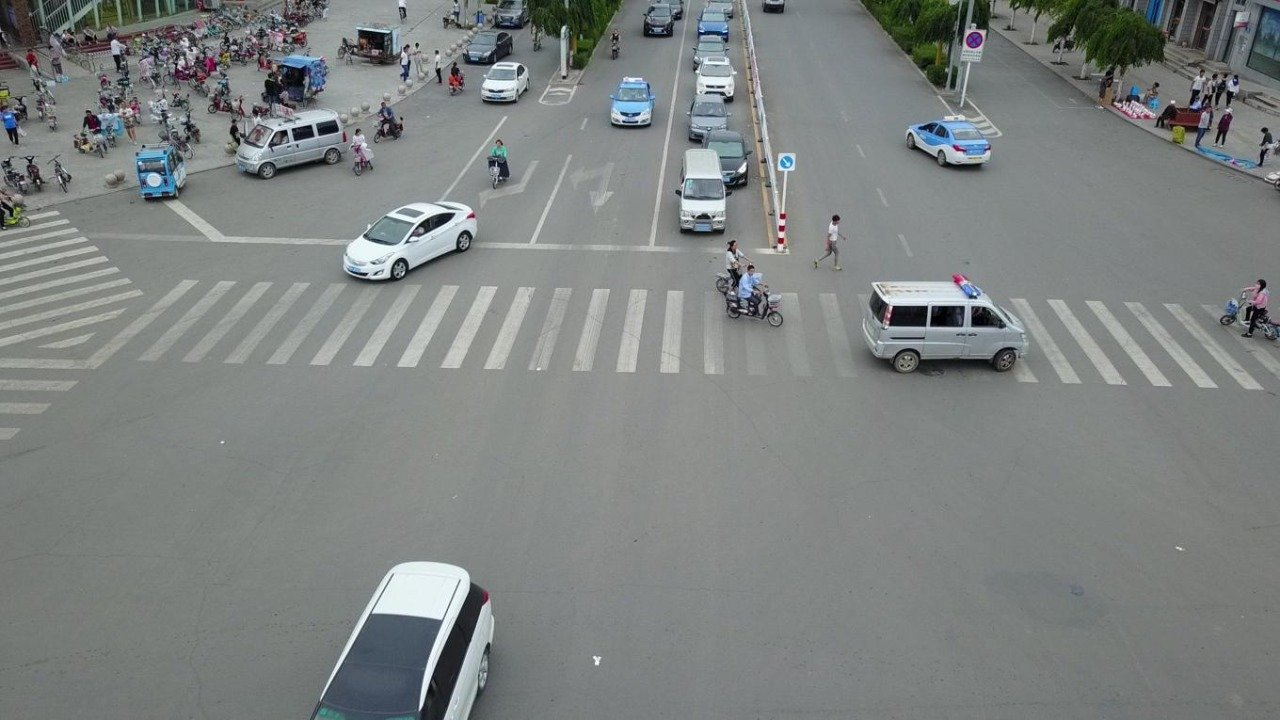
\includegraphics[width=\linewidth]{data_visdrone.jpg}\caption{VisDrone}\end{subfigure}\hfill
  \begin{subfigure}{0.32\linewidth}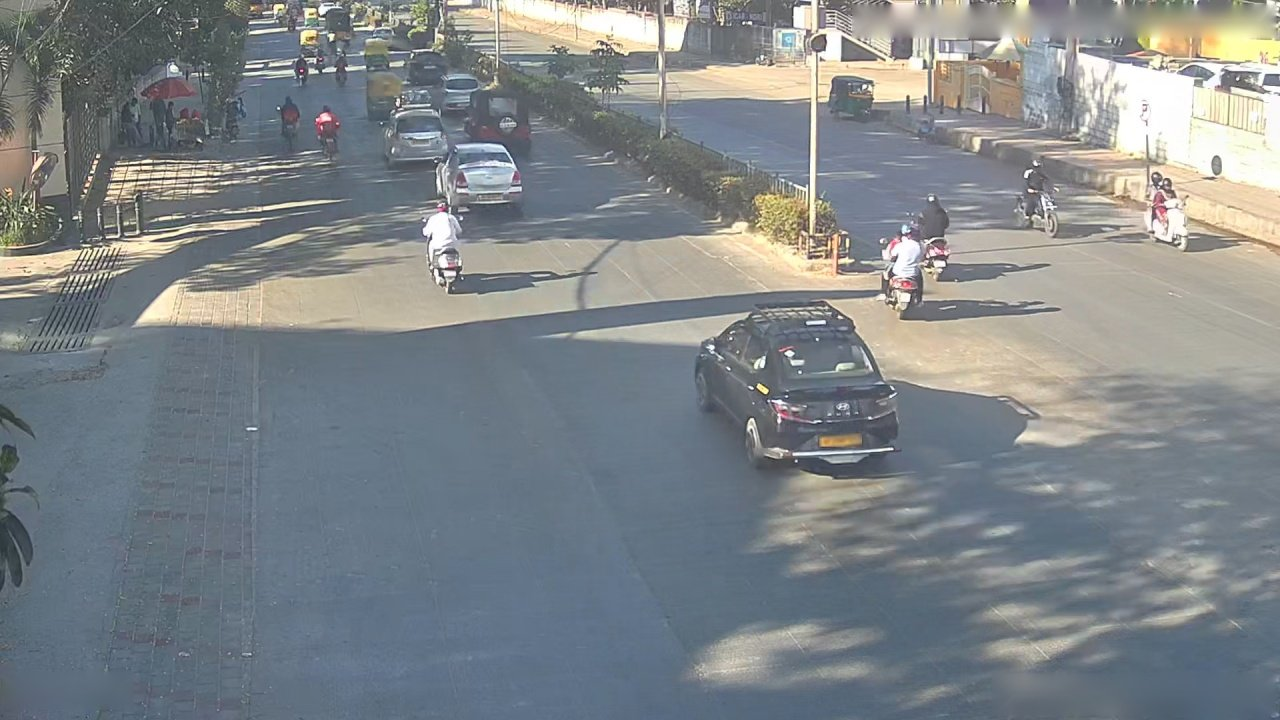
\includegraphics[width=\linewidth]{data_uvh26.jpg}\caption{UVH-26}\end{subfigure}\hfill
  \begin{subfigure}{0.32\linewidth}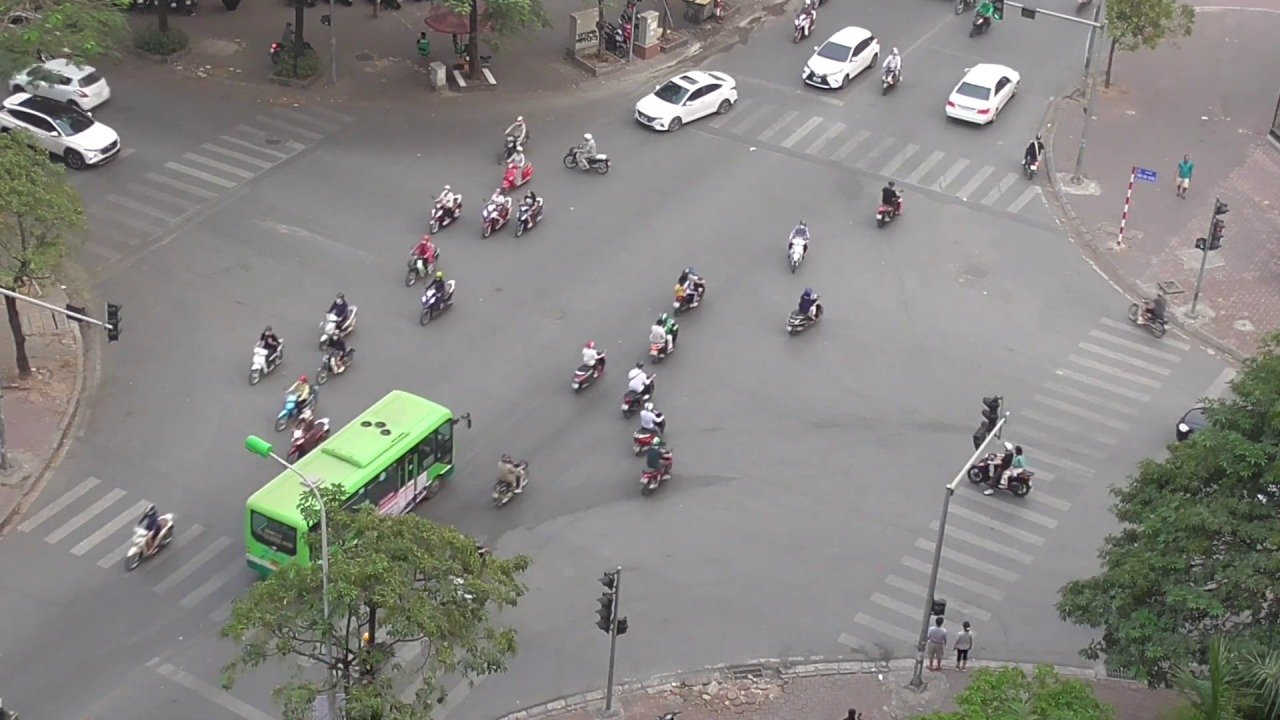
\includegraphics[width=\linewidth]{data_hanoi.jpg}\caption{Frame Hà Nội}\end{subfigure}
  \caption{Ví dụ ảnh từ sáu nguồn dữ liệu huấn luyện của v5}
  \label{fig:nguon-du-lieu}
\end{figure}

Lý do chọn từng nguồn gắn với các phiên bản mô hình ở mục~\ref{sec:cac-phien-ban}: VisDrone bù xe máy nhỏ nhìn từ trên
cao, frame Hà Nội bù đúng cảnh mục tiêu, UVH-26 là nguồn duy nhất đề tài tìm được có đúng góc camera giao thông trên
nhiều camera, còn frame đêm bù cảnh đường phố Việt Nam ban đêm (ví dụ ở Hình~\ref{fig:intro-traffic}b, phần Mở đầu).

\subsection{Chia tập huấn luyện, kiểm định và kiểm tra}
\label{sec:chia-tap}

Cách chia tập quyết định con số đánh giá có đáng tin hay không. Bộ \texttt{vehicle-vietnam-cantho} và
\texttt{vehicle-detection} gần như mỗi bộ chỉ có một camera, nếu chia ngẫu nhiên thì ảnh test và ảnh train là các frame
gần nhau của cùng một cảnh, mAP sẽ cao giả tạo. Vì vậy hai bộ này chỉ dùng để train. Tập val và test chỉ lấy từ bộ
\texttt{vietnamese-vehicle}, và đề tài không dùng cách chia sẵn của Roboflow. Các ảnh gần trùng nhau được gom thành nhóm
bằng mã băm cảm nhận dHash (hai ảnh có khoảng cách Hamming không quá 10 bit coi là cùng nhóm), rồi chia theo nhóm với
tỉ lệ 60/20/20 để không nhóm nào nằm ở hai tập. Ảnh được thu về cạnh dài tối đa 1280 điểm ảnh.

Frame Hà Nội được chia theo đoạn thời gian của video: 30 frame test lấy từ phút 0:35 đến 1:35 (mỗi 2 giây một frame),
10 frame val từ 1:45 đến 2:39, frame train lấy từ các đoạn sau đó. Cả ba phần đến từ \textbf{cùng một camera nhìn
xuống cùng một ngã tư}, chỉ khác thời điểm và mức zoom. Vì vậy với các mô hình đã học frame Hà Nội (v3 đến v6), tập test
Hà Nội đo độ chính xác \emph{trên chính camera đã dùng để tinh chỉnh}. Đây là một kịch bản triển khai có thật: camera
giao thông cố định, mô hình được tinh chỉnh bằng video của chính camera đó. Nhưng tập này không đo được khả năng tổng
quát sang camera mới. Khả năng tổng quát được đo trên các tập có camera không xuất hiện trong dữ liệu huấn luyện:
\texttt{vn\_extra}, clip Phạm Văn Đồng, val UVH-26 (đã bỏ ảnh cùng camera) và UA-DETRAC. Các clip Phạm Văn Đồng và hầm
chui chỉ dùng để test, không frame nào của chúng được đưa vào huấn luyện; frame đêm của v6 lấy từ hai camera khác.

Hai video đêm dùng để lấy frame huấn luyện là các đoạn ngắn được ghép lặp lại thành video dài (đoạn ở phút 15, phút 95
và phút 175 của một video có cùng nội dung). Frame được lấy 4 giây một lần trên mười đoạn hai phút, rồi bỏ những frame
gần trùng với frame đã lấy (chênh lệch điểm ảnh trung bình dưới 2 trên thang 0--255, sau khi thu nhỏ về 160×90; trên
video hầm chui, cặp frame trùng thật chênh 0.4--1.6). Các đoạn lặp lệch pha nhau nên bộ lọc chỉ bỏ 12 frame, còn 288
frame. Số cảnh giao thông thật sự khác nhau trong 288 frame này vì thế ít hơn con số 288.

Bảng~\ref{tab:thong-ke} là thống kê bộ dữ liệu phiên bản v6 (bản dùng cho mô hình triển khai): 5.002 ảnh train, 320 ảnh
val và 308 ảnh test. Bộ v5 giống hệt, chỉ thiếu dòng frame đêm (4.714 ảnh train).

\begin{table}[H]
  \centering
  \caption{Thống kê bộ dữ liệu v6 theo nguồn (số ảnh và số box mỗi lớp)}
  \label{tab:thong-ke}
  \small
  \begin{tabularx}{\linewidth}{|c|L|r|r|r|r|r|}
    \hline
    \thead{Tập} & \thead{Nguồn} & \thead{Ảnh} & \thead{Xe máy} & \thead{Ô tô} & \thead{Buýt} & \thead{Tải} \\ \hline
    train & cantho & 300 & 878 & 842 & 15 & 68 \\ \hline
    train & vehicle-detection & 300 & 2.181 & 844 & 49 & 51 \\ \hline
    train & vietnamese-vehicle & 929 & 1.328 & 1.629 & 197 & 1.123 \\ \hline
    train & VisDrone & 909 & 18.050 & 28.702 & 472 & 1.801 \\ \hline
    train & Hà Nội (69 frame × 4) & 276 & 18.192 & 4.256 & 68 & 100 \\ \hline
    train & UVH-26 & 2.000 & 12.348 & 7.066 & 1.231 & 3.351 \\ \hline
    train & Frame đêm (chỉ v6) & 288 & 6.256 & 3.811 & 162 & 148 \\ \hline
    val & vietnamese-vehicle & 310 & 451 & 579 & 93 & 352 \\ \hline
    val & Hà Nội & 10 & 889 & 156 & 7 & 1 \\ \hline
    test & vietnamese-vehicle & 308 & 453 & 609 & 115 & 303 \\ \hline
  \end{tabularx}
\end{table}

Xe máy và ô tô chiếm phần lớn số box; xe buýt và xe tải ít hơn nhiều. Đề tài không dùng trọng số lớp: mặc định của
Ultralytics không bật trọng số lớp, và trên tập test Roboflow (có nhiều buýt, tải) AP của hai lớp này không thấp hơn
xe máy (mục~\ref{sec:ket-qua-phat-hien}).

\subsection{Các tập đánh giá}
\label{sec:tap-danh-gia}

Tập test Roboflow không đại diện cho video mục tiêu (mục~\ref{sec:kho-khan}), nên đề tài tự xây thêm các tập đánh giá
Việt Nam và dùng thêm ba bộ dữ liệu bên ngoài (Bảng~\ref{tab:tap-danh-gia}).

\begin{table}[H]
  \centering
  \caption{Các tập đánh giá và vai trò (số box theo thứ tự xe máy / ô tô / buýt / tải)}
  \label{tab:tap-danh-gia}
  \small
  \begin{tabularx}{\linewidth}{|p{2.6cm}|L|p{2.9cm}|p{2.2cm}|}
    \hline
    \thead{Tập} & \thead{Nội dung} & \thead{Quy mô} & \thead{Vai trò} \\ \hline
    Val Hà Nội & 10 frame video ngã tư Hà Nội, nhãn người & 889 / 156 / 7 / 1 & Dev: chọn mô hình \\ \hline
    Test Hà Nội & 30 frame ngã tư Hà Nội, nhãn người (sơ bộ từ v2); cùng camera với frame train của v3--v6 & 2.982 /
      539 / 5 / 2 & Test phát hiện trên camera đã học \\ \hline
    \texttt{vn\_extra} ngày & 30 frame hai góc máy đại lộ Phạm Văn Đồng, nhãn người (sơ bộ từ YOLO26x) & 552 / 156 /
      0 / 2 & Test phát hiện \\ \hline
    \texttt{vn\_extra} đêm & 30 frame hầm chui TP.HCM ban đêm, nhãn người (sơ bộ từ YOLO26x) & 468 / 157 / 6 / 9 & Test
      phát hiện \\ \hline
    Dev đêm & 32 frame nút giao Công viên Gia Định (TP.HCM) ban đêm, YouTube kênh Vietnam Naturally; nhãn người (sơ bộ
      từ YOLO26x), 20 vùng bỏ qua; camera không có trong dữ liệu huấn luyện & 359 / 162 / 3 / 0 & Dev: nhận v6, chọn
      ngưỡng nhãn tự động ban đêm \\ \hline
    20 frame PVD & 1 frame mỗi giây của clip theo dõi & 375 / 238 / 12 / 0 & Test phát hiện \\ \hline
    Clip theo dõi PVD & 20 giây (600 frame, 30 fps), nhãn quỹ đạo bằng CVAT & 183 quỹ đạo & Test theo dõi, đếm xe
      ban ngày \\ \hline
    Đếm xe hầm chui & Hai clip đêm 60 giây, người đếm tay từng lượt qua vạch & 176 lượt: 149 / 25 / 1 / 1 & Test đếm xe
      ban đêm \\ \hline
    VnTraffic~\cite{le2026vntraffic} & Video giao thông Việt Nam (nguồn kênh HTV), nhìn chéo từ trên cao, 17 giây & 501
      frame, 85 quỹ đạo
      & Dev: chọn tracker \\ \hline
    Val UVH-26 & 509 ảnh, bỏ ảnh cùng camera với ảnh train & 2.973 / 1.239 / 219 / 546 & Chấm phụ \\ \hline
    UA-DETRAC~\cite{wen2020uadetrac, patrikskalos_uadetrac} & Camera cầu vượt Trung Quốc, 960×540; 21 video đêm và 39
      video ngày, 1 frame mỗi 100 frame & Đêm 51 / 1.578 / 143 / 21; ngày 35 / 4.003 / 246 / 19 & Chấm phụ đêm–ngày
      \\ \hline
    Test Roboflow & 308 ảnh \texttt{vietnamese-vehicle} & 453 / 609 / 115 / 303 & Chấm phụ \\ \hline
  \end{tabularx}
\end{table}

Ba tập dev được dùng để ra quyết định; mọi tập còn lại chỉ dùng để báo cáo. Một số lưu ý khi đọc các tập này:
\begin{itemize}
  \item \textbf{Val UVH-26.} UVH-26 chia train/val theo ảnh chứ không theo camera, nên đề tài lấy 800 ảnh val ngẫu
        nhiên rồi bỏ 291 ảnh có camera trùng với ảnh train đã dùng (so bằng dHash 256 bit, ngưỡng chọn bằng mắt), còn
        509 ảnh. Tập này đo khả năng tổng quát sang camera mới trong cùng miền Ấn Độ, không phải sang Việt Nam.
  \item \textbf{VnTraffic} là bộ nhãn theo dõi duy nhất tìm được đúng phạm vi, nhưng nhãn không đầy đủ: mỗi frame thiếu
        khoảng 6--9 xe mà mô hình phát hiện chắc chắn, và 55/85 quỹ đạo bị mất box 1--19 frame giữa chừng dù xe vẫn
        thấy rõ (đề tài lấp các khoảng này bằng box trung tính). Hệ quả là phát hiện thừa bị thổi phồng; trên tập này chỉ
        dùng AssA, IDR và số lần đổi ID để so tracker, vì ba chỉ số này không bị phạt khi phát hiện thêm xe.
  \item \textbf{UA-DETRAC} dùng bản nhãn gán lại có xe máy; điều kiện đêm hay ngày lấy theo thuộc tính thời tiết trong
        nhãn gốc (bỏ 11 video mưa). Đây là đường phố có đèn ở Trung Quốc, chủ yếu ô tô.
  \item \textbf{Dev đêm} được xây khi làm v6, vì hai tập dev cũ đều là cảnh ban ngày. Frame lấy 15 giây một lần từ bốn
        đoạn hai phút ở phút 40, 50, 58 và 64 của một video liền mạch, đều sau khi trời tối hẳn. Người gán thêm 248 box so với nhãn sơ bộ, phần lớn là
        xe máy nhỏ ở xa; 200 trong 524 xe cao dưới 32 điểm ảnh.
  \item \textbf{Video hầm chui.} Ba clip đêm được cắt ở ba thời điểm khác nhau của một video dài khoảng ba giờ, nhưng
        khi đếm xe từng frame mới thấy video gốc có đoạn lặp: frame 0--1387 của clip thứ nhất trùng frame 412--1799 của
        clip thứ hai (so chênh lệch điểm ảnh giữa các cặp frame), và clip thứ nhất có một chỗ cắt cảnh ở giây 48.3. Clip
        thứ hai và thứ ba liền mạch, không trùng nhau. Vì vậy tập \texttt{vn\_extra} đêm và phép đánh giá đếm xe ban đêm
        chỉ dùng clip thứ hai và thứ ba; clip thứ nhất chỉ để minh hoạ.
\end{itemize}

\section{Gán nhãn dữ liệu}

\subsection{Công cụ và quy trình}

Nhãn ảnh được gán bằng X-AnyLabeling, nhãn quỹ đạo video bằng CVAT. Gán từ đầu một frame có hơn 100 xe máy mất rất
nhiều thời gian, nên mọi tập đều theo quy trình ba bước: mô hình tạo nhãn sơ bộ, người gán sửa từng box, rồi một mô hình
khác rà soát để chỉ ra chỗ ``có thể sót'' và ``có thể thừa'' cho người gán xem lại.

Nhãn sơ bộ để lại dấu: box được người giữ nguyên mang cách khoanh của mô hình tạo ra nó. Với tập test Hà Nội, 69\% số
box là box sơ bộ của v2 giữ nguyên (IoU $\ge$ 0.95). Vì vậy với các tập test mới (\texttt{vn\_extra}), nhãn sơ bộ và rà
soát đều dùng YOLO26x gốc COCO, một mô hình không tham gia so sánh, để không ưu ái mô hình nào. Ảnh hưởng của dấu vết
này lên kết quả được bàn ở mục~\ref{sec:thao-luan}.

\subsection{Quy tắc gán nhãn}

\begin{itemize}
  \item Box xe máy bao cả người lái; xe bị che một phần được khoanh phần nhìn thấy.
  \item Chỉ gán nhãn một xe khi nhìn riêng frame đó xác định được đó là loại xe gì và nằm từ đâu đến đâu. Trường hợp mơ
        hồ (bị cây che gần hết, cụm xe quá xa) gán lớp \texttt{ignore} chứ không xoá, theo quy ước vùng bỏ qua của KITTI,
        COCO và VisDrone. Khi huấn luyện, box \texttt{ignore} bị bỏ vì Ultralytics không hỗ trợ vùng bỏ qua; khi chấm, chúng
        trở thành vùng \texttt{iscrowd}.
  \item \textbf{Xe van} được phân theo hình dáng thân xe, vì từ camera không biết xe chở người hay hàng: van nhỏ (Suzuki
        Blind Van, Towner, Tera V) và xe MPV 7 chỗ là ô tô; van cỡ Ford Transit mui cao, cả bản 16 chỗ lẫn bản chở hàng, là
        xe buýt. Quy tắc này khớp cách dữ liệu train v5 ánh xạ lớp (UVH-26 \texttt{Van} thành ô tô,
        \texttt{Tempo-traveller} và \texttt{Mini-bus} thành buýt). Nó lệch luật Việt Nam (van chở hàng là xe tải) và lệch
        KITTI, UA-DETRAC (có lớp van riêng), vì đề tài chỉ có bốn lớp.
  \item \textbf{Xe bán tải} năm chỗ (kiểu Ford Ranger) là ô tô. COCO xếp xe bán tải vào lớp xe tải, nhưng mọi mô hình
        của đề tài đều gọi loại xe này là ô tô, tức dữ liệu huấn luyện đã ngầm xếp nó vào ô tô, và ở Việt Nam xe bán tải
        chủ yếu dùng chở người. Theo quy ước COCO, hai lượt xe bán tải trong dữ liệu đếm ban đêm sẽ thành lỗi sai lớp
        của cả hai mô hình.
\end{itemize}

\subsection{Nhãn tự động cho frame huấn luyện}

69 frame train Hà Nội được gán nhãn tự động bằng cách ghép dự đoán của nhiều mô hình ``thầy'': v2 ở ảnh 960 và 1280,
YOLO26x ở ảnh 1280, và v2 chạy theo lát cắt SAHI~\cite{akyon2022sahi} 2×2 để bắt xe nhỏ; mỗi mô hình chạy thêm trên
ảnh lật ngang. Các box được ghép bằng Weighted Boxes Fusion~\cite{solovyev2021wbf}: box của các mô hình chồng lên nhau
được gộp thành một box có toạ độ là trung bình có trọng số theo điểm tin cậy. Box có điểm sau ghép từ 0.15 trở lên
được giữ; ngưỡng này chọn trên tập val Hà Nội có nhãn người, không nhìn tập test.

Đo trên val Hà Nội, nhãn tự động đạt Precision 0.905, Recall 0.853, F1 0.878; recall của xe máy là 0.841, cao hơn bản
không dùng SAHI (0.802). Phần bị sót chủ yếu là cụm xe máy dừng đèn đỏ.

288 frame đêm của v6 được gán nhãn theo cùng cách, với bộ thầy mạnh hơn: RT-DETRv2-S ở ảnh 960 (quá chậm để triển khai
nhưng dùng làm thầy được), YOLO26x ở ảnh 1280, v5 ở ảnh 960 và 1280, và v5
chạy theo lát cắt 2×2. Ngưỡng giữ box được chọn trên tập dev đêm (32 frame nhãn người, camera không có trong
frame train). Trên tập này, bản thêm lát cắt 2×2 cho mAP50 chính 0.800, cao hơn bản không cắt (0.778) và cao hơn thầy
mạnh nhất đứng riêng (RT-DETRv2-S, 0.702). F1 cao nhất là 0.712 ở ngưỡng 0.20 (Precision 0.81, Recall 0.63), nên ngưỡng
0.20 được dùng. Nhãn đêm thiếu nhiều hơn nhãn Hà Nội: xe cao từ 64 điểm ảnh trở lên được giữ khoảng 95\%, nhưng xe cao
dưới 32 điểm ảnh chỉ khoảng 40\%. Phần xe nhỏ bị sót trong nhãn là rủi ro của v6, vì mô hình có thể học rằng xe nhỏ ở
xa là nền; tiêu chí nhận v6 (mục~\ref{sec:tieu-chi-chon}) được đặt để phát hiện trường hợp đó.

\subsection{Bổ sung nhãn UVH-26}

Khi kiểm tra UVH-26, đề tài thấy nhãn thiếu ít nhất 15\% số xe, chủ yếu xe ở xa. Nhãn thiếu làm mô hình học rằng xe ở xa
là nền. Đề tài bổ sung bằng YOLO26x: dự đoán có điểm từ 0.5 trở lên ở chỗ chưa có box được thêm vào; dự đoán nằm quá
50\% trong một box đã có (kể cả box của lớp bị bỏ như xe ba bánh) bị loại để không tạo box trùng.

\subsection{Nhãn quỹ đạo cho clip test}

Clip test theo dõi dài 20 giây (giây 20--40 của clip \texttt{pvd\_goc\_a}, 600 frame). Nhãn sơ bộ là quỹ đạo do chính
tracker sinh ra, xuất sang CVAT với keyframe mỗi 10 frame; người gán kiểm từng quỹ đạo, sửa box và ID. Sau đó nhãn
được soát lại mà không dùng mô hình của đề tài: dải xa phía trên ảnh (toạ độ y nhỏ hơn 462, nơi xe máy cao dưới 25 điểm
ảnh theo ngưỡng của KITTI) là vùng bỏ qua; 20 quỹ đạo được kéo dài tới dải đó bằng so khớp mẫu; 14 chỗ quỹ đạo bị đứt
oan được nối lại; 121 box ``mảnh vụn'' của xe khuất sau cây được chuyển sang trạng thái không hiện diện sau khi xem
bằng mắt.
YOLO26x chỉ dùng để soát chéo. Mọi chỉnh sửa và lý do được ghi lại để truy ngược. Kết quả là 183 quỹ đạo.

\subsection{Nhãn đếm xe ban đêm}
\label{sec:nhan-dem}

Hai clip hầm chui chưa có nhãn quỹ đạo, nên số lượt xe thật được đếm tay trên video gốc, không hiện kết quả của mô hình.
Đây cũng là cách cuộc thi AI City Challenge tạo nhãn cho bài đếm xe. Đề tài viết một công cụ nhỏ: video phát chậm
0.25 lần, có vẽ vạch đếm (nằm ngang ở 60\% chiều cao ảnh, trùng vạch của hệ thống); mỗi khi điểm giữa đáy xe chạm vạch,
người đếm bấm một phím theo lớp và hướng, công cụ ghi lại frame đang hiện. Xe đã ở phía trên vạch khi clip bắt đầu, hoặc
chưa tới vạch khi clip kết thúc, không được tính. Bộ đếm của hệ thống cũng lấy điểm giữa đáy box làm điểm neo, nên
người đếm và hệ thống đo cùng một sự kiện.

Để kiểm tra độ tin cậy của nhãn, một trợ lý AI đếm độc lập trên cùng hai clip bằng cách xem ảnh gốc, không dùng mô hình
của đề tài. Hai bộ đếm ghép được 174 trên 176 lượt (lệch thời điểm trung vị 0.2 giây); trong đó chỉ hai lượt khác lớp,
đều là xe bán tải mà bộ đếm AI xếp vào xe tải theo COCO. Hai lượt còn lại là hai xe máy ở giây cuối của clip thứ ba mà
bộ đếm AI chưa chốt; xem phóng to các frame cuối cho thấy cả hai đều qua vạch trước khi clip kết thúc, nên được giữ theo
người đếm. Kết quả là 176 lượt, cùng một chiều: 149 xe máy, 25 ô tô, 1 xe buýt, 1 xe tải.

\section{Huấn luyện mô hình phát hiện}

\subsection{Cấu hình huấn luyện}

Mọi mô hình được huấn luyện trên GPU Tesla T4 của Kaggle, khởi tạo từ trọng số đã huấn luyện trên COCO. Cấu hình chung
cho YOLO26:
\begin{itemize}
  \item tối đa 100 epoch, dừng sớm nếu mAP50-95 trên val không tăng sau 20 epoch; seed 42 (để đo dao động giữa các lần
        huấn luyện, v5 và YOLO26s được huấn luyện thêm với seed 1 và 2, v6 với seed 1);
  \item kích thước ảnh 960 (v1 dùng 640, v4 dùng 1280); batch 16, cộng dồn gradient tới batch danh nghĩa 64;
  \item optimizer chọn tự động: số vòng lặp dự kiến với bộ dữ liệu v5 là $\lceil 4714 / 64 \rceil \times 100 = 7.400$,
        với v6 là $\lceil 5002 / 64 \rceil \times 100 = 7.900$, đều dưới 10.000, nên Ultralytics chọn AdamW với tốc độ
        học 0.00125;
  \item tăng cường dữ liệu mặc định (ghép 4 ảnh mosaic, đổi màu HSV, lật, co giãn, dịch), tắt mosaic ở 10 epoch cuối;
  \item lưu trọng số trung bình trượt EMA; chọn checkpoint có mAP50-95 val cao nhất; huấn luyện độ chính xác hỗn hợp.
\end{itemize}

\subsection{Quá trình cải tiến qua các phiên bản}
\label{sec:cac-phien-ban}

Mô hình được cải tiến qua sáu phiên bản dữ liệu, mỗi lần chỉ đổi một yếu tố để biết thay đổi nào có tác dụng
(Bảng~\ref{tab:lich-su-train}).

\begin{table}[H]
  \centering
  \caption{Lịch sử huấn luyện các mô hình (val và test Roboflow do bộ chấm của thư viện tính khi train)}
  \label{tab:lich-su-train}
  \footnotesize
  \begin{tabularx}{\linewidth}{|p{1.5cm}|L|>{\centering\arraybackslash}p{0.8cm}|>{\centering\arraybackslash}p{1.5cm}|>{\centering\arraybackslash}p{1.7cm}|>{\centering\arraybackslash}p{1.8cm}|>{\centering\arraybackslash}p{0.9cm}|}
    \hline
    \thead{Mô hình} & \thead{Dữ liệu train} & \thead{Ảnh} & \thead{Epoch tốt nhất / đã chạy} &
      \thead{Val mAP50 / 50-95} & \thead{Test Roboflow mAP50 / 50-95} & \thead{Giờ T4} \\ \hline
    v1 & Roboflow + VisDrone & 640 & 81 / 100 & 0.831 / 0.549 & 0.861 / 0.572 & 0.84 \\ \hline
    v2 & cantho, vehicle-detection 300 ảnh mỗi bộ; VisDrone 909 ảnh nhiều xe máy & 960 & 86 / 100 & 0.838 / 0.555 &
      0.864 / 0.573 & 1.61 \\ \hline
    v3 & v2 + 69 frame Hà Nội nhãn tự động + 10 frame val & 960 & 80 / 100 & 0.853 / 0.616 & 0.870 / 0.573 & 1.79 \\ \hline
    v4 & như v3 & 1280 & 83 / 100 & 0.851 / 0.616 & 0.873 / 0.575 & 3.18 \\ \hline
    v5 & v3 + 2.000 ảnh UVH-26 & 960 & 90 / 100 & 0.867 / 0.628 & 0.861 / 0.578 & 2.96 \\ \hline
    v5, seed 1 & như v5 & 960 & 69 / 89 & 0.877 / 0.638 & 0.868 / 0.590 & 2.68 \\ \hline
    v5, seed 2 & như v5 & 960 & 93 / 100 & 0.871 / 0.630 & 0.862 / 0.579 & 3.02 \\ \hline
    \textbf{v6} & v5 + 288 frame đêm nhãn tự động & 960 & 73 / 93 & 0.868 / 0.629 & 0.868 / 0.584 & 3.04 \\ \hline
    v6, seed 1 & như v6 & 960 & 85 / 100 & 0.862 / 0.626 & 0.858 / 0.587 & 3.27 \\ \hline
    YOLO26s & như v5 & 960 & 87 / 100 & 0.873 / 0.639 & 0.884 / 0.600 & 4.90 \\ \hline
    YOLO26s, seed 1 & như v5 & 960 & 81 / 100 & 0.875 / 0.644 & 0.879 / 0.594 & 5.36 \\ \hline
    YOLO26s, seed 2 & như v5 & 960 & 60 / 80 & 0.873 / 0.647 & 0.887 / 0.603 & 4.31 \\ \hline
    RT-DETRv2-S & như v5 & 960 & 61 / 81 & 0.878 / 0.651 & 0.874 / 0.601 & 10.7 \\ \hline
  \end{tabularx}
\end{table}

Lý do của từng bước:
\begin{itemize}
  \item \textbf{v1} đạt mAP50 0.861 trên test Roboflow, nhưng trên frame Hà Nội gần như không bắt được xe máy (AP50 xe
        máy 0.045), còn kém mô hình gốc COCO. Tập test Roboflow không đại diện cho cảnh mục tiêu, nên từ đây mọi mô
        hình đều được chấm thêm trên frame Việt Nam tự gán.
  \item \textbf{v2} tăng kích thước ảnh lên 960 và thêm ảnh VisDrone có nhiều xe máy nhỏ nhìn từ trên cao. Trên 5
        frame Hà Nội, v2 bắt được 405 xe máy so với 167 của mô hình COCO ở ảnh 1280 và 12 của v1.
  \item \textbf{v3} thêm frame Hà Nội gán nhãn tự động, tức đúng cảnh mục tiêu (lặp 4 lần để đủ trọng số).
  \item \textbf{v4} thử tăng ảnh lên 1280. Trên val Hà Nội không tốt hơn v3 (0.916 so với 0.917) mà chậm hơn, nên giữ v3.
  \item \textbf{v5} thêm 2.000 ảnh UVH-26 có đúng góc camera giao thông. Khi phân tích các xe v3 bỏ sót trên VnTraffic
        (một xe buýt bị che một phần, một xe tải nhìn xiên, xe máy dừng nhìn thẳng), đề tài thấy v3 không nhận ra chúng ở
        mọi kích thước ảnh, trong khi dữ liệu train đã có hàng trăm xe buýt và hàng nghìn xe tải. Nguyên nhân là thiếu ảnh
        đúng góc camera giao thông chứ không thiếu lớp; v5 nhận ra được các xe này.
  \item \textbf{v6} thêm 288 frame đêm từ hai camera mới, gán nhãn tự động. Hướng này xuất phát từ kết quả của v5: ban
        đêm là cảnh v5 yếu nhất và dao động mạnh nhất giữa các lần huấn luyện (mục~\ref{sec:thao-luan}). Frame đêm lấy từ camera
        khác với clip hầm chui dùng để test.
\end{itemize}

Hai mô hình YOLO26s và RT-DETRv2-S dùng đúng dữ liệu v5 để so sánh kiến trúc (mục~\ref{sec:giao-thuc}). Hình~\ref{fig:hoc}
là đường học trên tập val của ba mô hình cùng dữ liệu v5. RT-DETRv2-S hội tụ sớm hơn, gần như không tăng từ khoảng
epoch 55, nên bị dừng sớm ở epoch 81, trước pha tắt tăng cường dữ liệu ở 10 epoch cuối mà hai bản YOLO đều trải qua.

\begin{figure}[H]
  \centering
  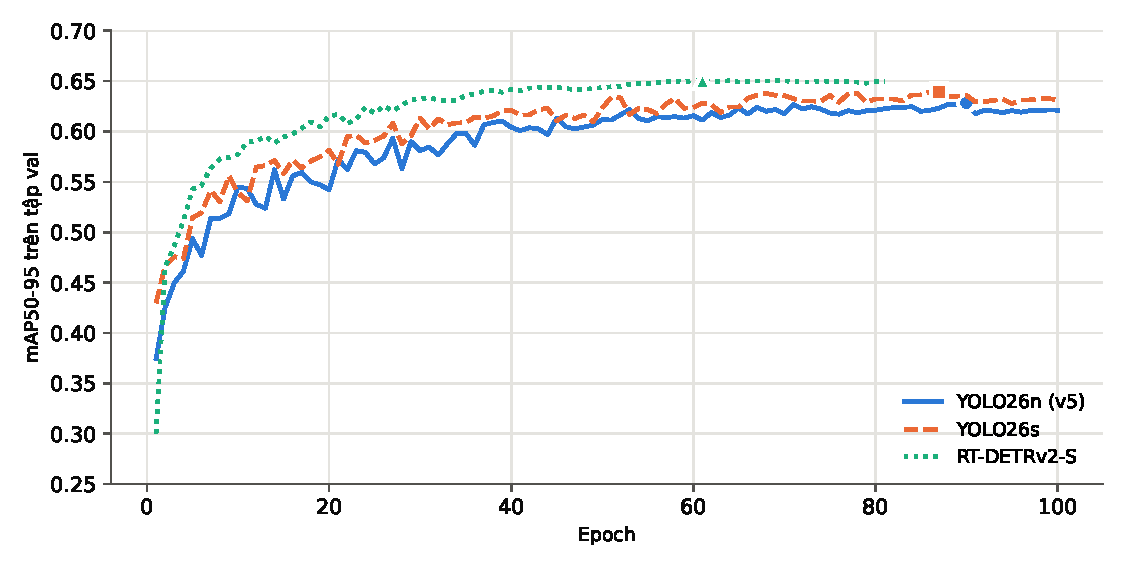
\includegraphics[width=0.92\linewidth]{learning_curves.pdf}
  \caption{mAP50-95 trên tập val theo epoch của ba mô hình huấn luyện trên dữ liệu v5; điểm đánh dấu là epoch được
           chọn. Số của YOLO do bộ chấm Ultralytics tính, số của RT-DETRv2 do pycocotools tính, nên chỉ so được hình
           dạng đường học}
  \label{fig:hoc}
\end{figure}

\subsection{Tiêu chí chọn mô hình}
\label{sec:tieu-chi-chon}

Tiêu chí được đặt trước khi chạy: với mô hình phát hiện, so mAP50 chính trên val Hà Nội; với tác động lên theo dõi, so
IDR trên VnTraffic; chênh lệch dưới 0.005 điểm là hoà và khi hoà chọn phương án nhanh hơn. Theo tiêu chí này:
\begin{itemize}
  \item \textbf{v5 được chọn thay v3}: mAP50 val hoà (0.919 so với 0.917) nhưng trên VnTraffic IDR tăng từ 0.744 lên
        0.827 và số lần đổi ID giảm từ 128 xuống 62. Hai lần huấn luyện lại v5 với seed khác sau đó cho cùng kết luận
        (mục~\ref{sec:thao-luan}).
  \item \textbf{Giữ ảnh 960 cho v5}, không dùng 1280: mAP50 val hoà (0.922 so với 0.919), trên VnTraffic bản 1280 đổi
        ID nhiều hơn (85 so với 62) và chậm hơn khoảng 1.5 lần.
\end{itemize}

Với v6, vì độ chính xác ban đêm dao động mạnh giữa các lần huấn luyện, tiêu chí được viết ra trước khi huấn luyện v6
và tính trên cả hai lần huấn luyện (seed 42 và 1), so với ba lần huấn luyện của v5. v6 được nhận nếu đạt đủ ba điều
kiện; nếu không, giữ v5 và báo cáo kết quả âm tính. Kết quả:
\begin{enumerate}
  \item mAP50 chính trên dev đêm của cả hai lần v6 phải cao hơn lần tốt nhất của v5 (0.499; ba lần v5 đạt 0.499, 0.498
        và 0.464): v6 đạt 0.599 và 0.618, \textbf{đạt}.
  \item mAP50 chính trên val Hà Nội của mỗi lần v6 không thấp hơn lần kém nhất của v5 quá 0.005 (tức từ 0.909 trở lên):
        cả hai lần đạt 0.914, \textbf{đạt}.
  \item IDR trên VnTraffic của mỗi lần v6 không thấp hơn lần kém nhất của v5 quá 0.005 (từ 0.822 trở lên): 0.841 và
        0.824, \textbf{đạt}, lần thứ hai sát ngưỡng.
\end{enumerate}
Mô hình triển khai là \textbf{v6 với seed 42}, theo cùng quy ước với các phiên bản trước; lần huấn luyện với seed 1 chỉ
dùng để đo độ dao động.

\section{Giao thức so sánh kiến trúc CNN và Transformer}
\label{sec:giao-thuc}

Câu hỏi của thí nghiệm là: họ Transformer có phát hiện xe Việt Nam tốt hơn họ CNN không, và phải trả bao nhiêu về tốc
độ. Nguyên tắc là đồng nhất mọi yếu tố đồng nhất được mà không làm bên nào bị huấn luyện sai công thức của nó; yếu tố
nào gắn với kiến trúc thì mỗi bên giữ theo bản chính thức và ghi rõ. YOLO26 dùng mặc định của Ultralytics 8.4.163;
RT-DETRv2-S dùng cấu hình chính thức của tác giả cho bản ResNet-18, chạy qua thư viện Transformers.

\begin{table}[H]
  \centering
  \caption{Các yếu tố được đồng nhất giữa YOLO26 và RT-DETRv2-S}
  \label{tab:dong-nhat}
  \small
  \begin{tabularx}{\linewidth}{|p{4cm}|L|}
    \hline
    \thead{Yếu tố} & \thead{Cách giữ đồng nhất} \\ \hline
    Dữ liệu và nhãn & Cùng bộ v5 (4.714 train, 320 val, 308 test), cùng file nhãn \\ \hline
    Khởi tạo & Cả hai từ trọng số COCO, đầu phân lớp khởi tạo lại cho 4 lớp \\ \hline
    Kích thước ảnh & 960 \\ \hline
    Số epoch, dừng sớm & Tối đa 100; dừng khi mAP50-95 val không tăng sau 20 epoch \\ \hline
    Chọn checkpoint & Trọng số EMA có mAP50-95 val cao nhất; cùng công thức EMA \\ \hline
    Optimizer & AdamW ở cả hai; huấn luyện độ chính xác hỗn hợp; seed 42 \\ \hline
    Đầu ra & Tối đa 300 phát hiện mỗi ảnh, không NMS, không TTA \\ \hline
    Chấm điểm & Một đường chấm chung: pycocotools, ngưỡng tin cậy 0.001, tối đa 500 phát hiện mỗi ảnh, cùng vùng bỏ
      qua, cùng bootstrap \\ \hline
    Đo tốc độ và độ phức tạp & Cùng CPU, cùng frame, cùng giao diện (tiền xử lý + suy luận + hậu xử lý); GFLOPs đo bằng
      cùng công cụ ở đúng đầu vào thực tế \\ \hline
  \end{tabularx}
\end{table}

Ba yếu tố của RT-DETRv2 được chỉnh lệch bản chính thức cho giống YOLO: kích thước ảnh 640 thành 960; warmup tốc độ học
2.000 bước thành 3 epoch (2.000 bước là khoảng 0.27 epoch trên COCO nhưng gần 7 epoch trên 4.714 ảnh); tắt tăng cường
dữ liệu mạnh ở 10 epoch cuối thay vì 3.

Các yếu tố không thể đồng nhất vì gắn với công thức của từng họ được liệt kê trong Bảng~\ref{tab:khong-dong-nhat}.

\begin{table}[H]
  \centering
  \caption{Các yếu tố khác nhau giữa hai họ mô hình}
  \label{tab:khong-dong-nhat}
  \small
  \begin{tabularx}{\linewidth}{|p{2.8cm}|L|L|}
    \hline
    \thead{Yếu tố} & \thead{YOLO26} & \thead{RT-DETRv2-S} \\ \hline
    Tốc độ học & 0.00125, giảm tuyến tính & $10^{-4}$ cố định sau warmup, cắt gradient 0.1 \\ \hline
    Batch hiệu dụng & 64 (batch 16 hoặc 8, cộng dồn gradient) & 16 (8 × cộng dồn 2) \\ \hline
    Tăng cường dữ liệu & Mosaic, HSV, lật, co giãn & Biến đổi màu, ZoomOut, IoUCrop, lật \\ \hline
    Đưa ảnh về 960 & Giữ tỉ lệ, đệm viền: video 1080p thành 544×960 & Kéo giãn thành 960×960 \\ \hline
    Mất mát & BCE, box IoU, L1 & VFL, L1, GIoU, denoising \\ \hline
  \end{tabularx}
\end{table}

Batch không được ép bằng nhau vì nó gắn chặt với tốc độ học của từng công thức. Nếu ép YOLO về batch danh nghĩa 16, số
vòng lặp vượt 10.000 và Ultralytics tự đổi sang optimizer MuSGD với tốc độ học 0.01, tức YOLO bị huấn luyện theo công
thức khác. Hệ quả cần nhớ khi đọc kết quả: với video 16:9, YOLO nhìn 960×540 điểm ảnh có nội dung còn RT-DETRv2 nhìn
960×960, nhiều hơn khoảng 1.8 lần. Vì vậy đề tài chạy thêm một đối chứng: YOLO26s ở ảnh 1280 (1280×720 bằng khoảng
960×960 điểm ảnh).

Trước khi chấm chính thức, đường chấm được kiểm chứng trên 320 ảnh val. Với RT-DETRv2, đường chấm của đề tài cho mAP50
0.8785 và mAP50-95 0.6506, lệch dưới 0.001 so với nhật ký huấn luyện. Với YOLO26s, số thư viện in khi train (0.873)
cao hơn đường chấm của đề tài (0.847); nguyên nhân là chế độ chấm của Ultralytics đệm thêm viền ảnh. Khi chấm chính dự
đoán của Ultralytics bằng bộ chấm của đề tài thì ra 0.870, khớp 0.872, nên bộ chấm đúng. Đường chấm của đề tài đo đúng
cách mô hình chạy khi triển khai và áp dụng như nhau cho mọi mô hình.

\section{Theo dõi đối tượng và chọn tracker}
\label{sec:chon-tracker}

Đánh giá theo dõi dùng hai tập tách biệt: VnTraffic là tập dev để chọn tracker và chỉnh tham số; clip Phạm Văn Đồng
gán nhãn tay là tập test, dùng để chấm cấu hình đã chọn. Việc chấm không phân lớp (mọi xe là một lớp), vì tracker của
Ultralytics ghép box chỉ theo vị trí, không xét lớp; chất lượng phân loại đã được đo bằng mAP.

Quá trình chọn gồm bốn bước, kết quả chi tiết ở mục~\ref{sec:theo-doi}:
\begin{enumerate}
  \item So ByteTrack, BoT-SORT và OC-SORT với tham số mặc định: BoT-SORT tốt nhất trên cả AssA, IDR và số lần đổi ID.
  \item Chỉnh lưới tham số BoT-SORT (thời gian giữ track mất 30, 60 hay 90 frame; bật hay tắt ReID): chọn giữ track 90
        frame, không ReID. Bật ReID bằng đặc trưng của chính mô hình phát hiện làm số lần đổi ID tăng từ 128 lên khoảng
        208.
  \item Tắt bù chuyển động camera (GMC): camera trong phạm vi đề tài đứng yên, GMC chỉ ước lượng chuyển động gần bằng 0
        mà tốn thời gian; trên dev hai bản hoà nhau nên chọn bản nhanh hơn.
  \item Trong pipeline video, bỏ các track tồn tại dưới 3 frame (tương đương \texttt{min\_hits} của SORT) để giảm track
        rác; bộ chấm vẫn báo kết quả thô làm số chính.
\end{enumerate}

\begin{table}[H]
  \centering
  \caption{Cấu hình tracker mặc định của hệ thống (BoT-SORT đã chỉnh, không GMC)}
  \label{tab:tracker-config}
  \small
  \begin{tabularx}{\linewidth}{|p{4.2cm}|c|L|}
    \hline
    \thead{Tham số} & \thead{Giá trị} & \thead{Ý nghĩa} \\ \hline
    \texttt{track\_high\_thresh} & 0.25 & Ngưỡng box điểm cao cho lần ghép thứ nhất \\ \hline
    \texttt{track\_low\_thresh} & 0.1 & Ngưỡng dưới của box dùng ở lần ghép thứ hai \\ \hline
    \texttt{new\_track\_thresh} & 0.25 & Điểm tối thiểu để tạo track mới \\ \hline
    \texttt{track\_buffer} & 90 & Số frame giữ track bị mất trước khi xoá \\ \hline
    \texttt{match\_thresh} & 0.8 & Ngưỡng chi phí ghép cặp \\ \hline
    \texttt{gmc\_method} & none & Tắt bù chuyển động camera \\ \hline
    \texttt{with\_reid} & false & Không dùng đặc trưng ngoại hình \\ \hline
  \end{tabularx}
\end{table}

\section{Pipeline hệ thống và ứng dụng}

\subsection{Luồng xử lý}

Hình~\ref{fig:pipeline} là luồng xử lý mỗi frame. Toàn bộ logic nằm trong một hàm dùng chung cho chương trình dòng lệnh,
web demo và bộ chấm theo dõi, nên số liệu đo được đúng là thứ chạy trong demo.

\begin{figure}[H]
  \centering
  % Vẽ bằng TikZ ở report/figures_src/pipeline.tex, biên dịch sẵn thành PDF cho nhanh
  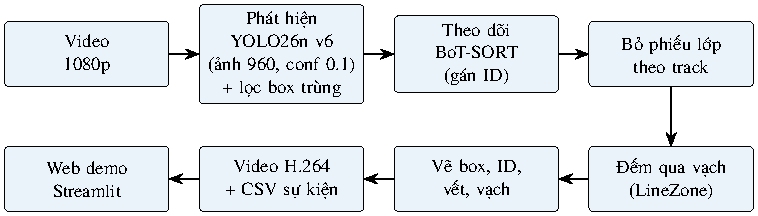
\includegraphics[width=\linewidth]{pipeline.pdf}
  \caption{Luồng xử lý của hệ thống}
  \label{fig:pipeline}
\end{figure}

Các bước:
\begin{enumerate}
  \item \textbf{Phát hiện và theo dõi.} Mỗi frame được đưa qua mô hình phát hiện với ngưỡng tin cậy 0.1 rồi qua BoT-SORT.
        Ngưỡng 0.1 để tracker có box điểm thấp cho lần ghép thứ hai; việc tạo track mới do \texttt{new\_track\_thresh}
        (0.25) quyết định. Ở frame đầu của mỗi video tracker được tạo mới, để chạy nhiều video liên tiếp trong web demo
        không bị dính ID cũ.
  \item \textbf{Ánh xạ lớp theo tên.} Tên lớp của mô hình được đổi sang bốn lớp chuẩn theo tên (ví dụ
        \texttt{motorcycle} thành \texttt{motorbike}), nên cùng một mã chạy được với mô hình COCO gốc và các mô hình
        tinh chỉnh.
  \item \textbf{Bỏ phiếu lớp theo track.} Một xe có thể bị gọi lúc là ô tô, lúc là xe tải giữa các frame. Lớp của mỗi
        track được chọn bằng bỏ phiếu có trọng số độ tin cậy:
\end{enumerate}
\begin{equation}
  \hat{c}(k) = \arg\max_{c} \sum_{t \in \mathcal{T}_k} s_t \cdot \mathbf{1}\{c_t = c\}
  \label{eq:vote}
\end{equation}
Công thức (\ref{eq:vote}): lớp của track $k$, với $\mathcal{T}_k$ là các frame track $k$ xuất hiện, $c_t$ và $s_t$ là
lớp và điểm tin cậy của box ở frame $t$. Lớp sau bỏ phiếu được ghi đè lên kết quả trước khi đếm, vì thư viện đếm theo lớp
tại thời điểm xe cắt vạch.
\begin{enumerate}[resume]
  \item \textbf{Đếm qua vạch.} Vạch đếm là một đoạn thẳng do người dùng đặt (mặc định nằm ngang ở 60\% chiều cao ảnh).
        Điểm giữa cạnh đáy của box được dùng làm điểm neo; khi điểm neo của một track đi từ bên này sang bên kia vạch,
        hệ thống ghi một sự kiện gồm frame, thời điểm, ID, lớp và hướng (vào hoặc ra).
  \item \textbf{Hiển thị và xuất kết quả.} Box được vẽ theo màu lớp, nhãn ``\#ID lớp'' chỉ ghi cho xe cao từ 4\% khung
        hình trở lên (xe nhỏ ở xa chỉ vẽ khung để chữ không đè nhau). ID hiển thị được đánh lại 1, 2, 3, \ldots theo thứ
        tự xe xuất hiện, vì ID gốc của tracker lên tới hàng nghìn do các track thử nghiệm bị huỷ vẫn tiêu số. Video được
        mã hoá lại sang H.264 để trình duyệt phát được; danh sách sự kiện xuất ra file CSV, kèm file cấu hình đã dùng.
\end{enumerate}

\subsection{Web demo và triển khai}

Web demo viết bằng Streamlit có hai chế độ. Chế độ chạy trực tiếp cho chọn clip có sẵn hoặc tải video lên, chọn mô hình,
tracker, ngưỡng tin cậy và vị trí vạch đếm, rồi hiển thị video kết quả, bảng đếm theo lớp và hướng, biểu đồ số xe cộng
dồn theo thời gian và cho tải file CSV. Chế độ thứ hai nạp lại video đã xử lý sẵn trên GPU, dùng khi trình chiếu vì
trên laptop, tính cả vẽ kết quả và ghi video 1080p, cả quy trình chỉ đạt khoảng 7 frame/s.

Để chạy nhanh trên laptop, mô hình triển khai được xuất sang OpenVINO~\cite{openvino}. Bản dùng cho web demo nhận ảnh
544×960, đúng khung video 16:9 với cạnh dài bằng kích thước ảnh lúc huấn luyện, và chạy trên GPU Intel tích hợp của
laptop. Cấu hình này được chọn khi v5 còn là mô hình triển khai; cách chọn và các phương án khác (INT8, chạy trên CPU)
trình bày ở mục~\ref{sec:openvino}. v6 dùng lại đúng cấu hình đó, vì cùng kiến trúc và cùng kích thước đầu vào.

\section{Kết luận chương}

Chương này đã trình bày cách xây dựng hệ thống. Dữ liệu huấn luyện gộp từ bảy nguồn, chia theo cảnh để tránh rò rỉ giữa
train và test; các tập đánh giá Việt Nam do đề tài tự gán nhãn, gồm cả cảnh đêm, một clip có nhãn quỹ đạo và hai clip
đêm có số lượt qua vạch do người đếm tay. Mô hình phát hiện được cải tiến qua sáu phiên bản dữ liệu, chọn bằng tiêu chí
đặt trước trên tập dev, và mô hình triển khai là YOLO26n v6, xuất sang OpenVINO để chạy trên GPU tích hợp của laptop.
Thí nghiệm so sánh với RT-DETRv2-S theo một giao thức ghi rõ các yếu tố đồng nhất và không đồng nhất được. Thuật toán
theo dõi được chọn là BoT-SORT đã chỉnh, không bù chuyển động camera. Chương~\ref{chap:ketqua} trình bày kết quả thực
nghiệm của các lựa chọn này.

\chapter{KẾT QUẢ THỰC NGHIỆM}
\label{chap:ketqua}

Chương này trình bày kết quả của bốn thí nghiệm: E1 đo độ chính xác phát hiện (gồm cả so sánh kiến trúc), E2 đo tốc độ,
E3 đo chất lượng theo dõi và sai số đếm xe, E4 phân tích các loại lỗi. Cuối chương là ứng dụng web, phần thảo luận và
kết luận. Mọi con số được lấy từ file kết quả của từng lần chạy.

\section{Tiêu chí và cách đánh giá}

\textbf{Phát hiện.} Chỉ số chính là mAP50 trung bình của xe máy và ô tô (mục~\ref{sec:chi-so}), kèm khoảng tin cậy
bootstrap 95\%. Mọi mô hình được chấm bằng cùng một đường chấm (pycocotools, ngưỡng tin cậy 0.001, tối đa 500 phát hiện
mỗi ảnh, có vùng bỏ qua), mỗi mô hình chạy ở đúng kích thước ảnh lúc huấn luyện. mAP50-95 chỉ được dùng trên các tập
mà nhãn sơ bộ không đến từ mô hình đang so sánh (\texttt{vn\_extra}, val UVH-26, UA-DETRAC); lý do ở
mục~\ref{sec:thao-luan}. Tập test Roboflow, val UVH-26 dùng cả bốn lớp; UA-DETRAC dùng xe máy, ô tô và xe buýt.

\textbf{Theo dõi.} Trên tập test (clip Phạm Văn Đồng) báo đủ HOTA, DetA, AssA, MOTA, IDF1, IDR, IDP và số lần đổi ID.
Trên tập dev VnTraffic chỉ dùng AssA, IDR và số lần đổi ID vì nhãn thiếu xe.

\textbf{Đếm xe.} So số lượt qua vạch theo lớp và hướng giữa hệ thống và nhãn tay.

\textbf{Tốc độ.} Thời gian xử lý mỗi frame (trung vị và khoảng tứ phân vị) trên CPU Intel Core i5-8250U và GPU Tesla T4.

\section{Kết quả phát hiện}
\label{sec:ket-qua-phat-hien}

\subsection{Tập test Hà Nội}

\begin{table}[H]
  \centering
  \caption{Kết quả phát hiện trên tập test Hà Nội (30 frame; 2.982 xe máy, 539 ô tô)}
  \label{tab:e1-hanoi}
  \small
  \begin{tabularx}{\linewidth}{|L|c|c|c|c|}
    \hline
    \thead{Mô hình} & \thead{Ảnh} & \thead{mAP50 chính [CI 95\%]} & \thead{AP50 xe máy} & \thead{AP50 ô tô} \\ \hline
    YOLO26n gốc COCO & 1280 & 0.686 [0.674--0.701] & 0.530 & 0.842 \\ \hline
    v1 & 640 & 0.395 [0.368--0.414] & 0.045 & 0.744 \\ \hline
    v2 & 960 & 0.890 [0.882--0.901] & 0.819 & 0.961 \\ \hline
    v3 & 960 & 0.921 [0.915--0.934] & 0.865 & 0.978 \\ \hline
    v4 & 1280 & 0.919 [0.910--0.927] & 0.862 & 0.975 \\ \hline
    \textbf{v5} & 960 & \textbf{0.923} [0.915--0.932] & 0.864 & 0.982 \\ \hline
  \end{tabularx}
\end{table}

Bảng~\ref{tab:e1-hanoi} cho thấy tinh chỉnh trên dữ liệu phù hợp nâng mAP50 chính từ 0.686 (mô hình gốc COCO, chạy ở
ảnh 1280) lên 0.923. Bước nhảy lớn nhất ở xe máy: AP50 từ 0.530 lên 0.864. Phiên bản v1, dù tốt trên
test Roboflow, kém cả mô hình gốc ở đây vì gần như không bắt được xe máy nhỏ. Ba bản v3, v4, v5 có khoảng tin cậy chồng
nhau, tức tập test Hà Nội không phân biệt được chúng; khác biệt giữa chúng thể hiện ở cảnh khó hơn và ở chất lượng
theo dõi.

\subsection{Cảnh mới ban ngày và ban đêm}

Tập \texttt{vn\_extra} gồm hai góc máy mới ban ngày (đại lộ dài, 52\% xe cao dưới 32 điểm ảnh) và cảnh đêm ở hầm chui.
Nhãn sơ bộ từ YOLO26x nên dùng được cả mAP50-95.

\begin{table}[H]
  \centering
  \caption{Kết quả phát hiện trên tập \texttt{vn\_extra} ngày và đêm}
  \label{tab:vn-extra}
  \footnotesize
  \begin{tabularx}{\linewidth}{|p{3.3cm}|C|>{\centering\arraybackslash}p{1.6cm}|C|>{\centering\arraybackslash}p{1.6cm}|}
    \hline
    \thead{Mô hình} & \thead{Ngày mAP50 [CI]} & \thead{Ngày mAP50-95} & \thead{Đêm mAP50 [CI]} & \thead{Đêm mAP50-95} \\ \hline
    YOLO26n gốc COCO @1280 & 0.458 [0.432--0.489] & 0.286 & 0.437 [0.396--0.499] & 0.308 \\ \hline
    v1 @640 & 0.081 & 0.035 & 0.183 & 0.106 \\ \hline
    v2 & 0.736 & 0.424 & 0.496 & 0.306 \\ \hline
    v3 & 0.757 & 0.460 & 0.437 & 0.263 \\ \hline
    v4 @1280 & \textbf{0.808} [0.779--0.824] & 0.517 & 0.481 & 0.321 \\ \hline
    \textbf{v5} & 0.745 [0.715--0.769] & 0.438 & \textbf{0.628} [0.598--0.659] & 0.404 \\ \hline
    v5 @1280 (chỉ phân tích) & 0.834 [0.808--0.842] & 0.519 & 0.657 [0.619--0.691] & 0.449 \\ \hline
  \end{tabularx}
\end{table}

Kết quả ban ngày và ban đêm khác nhau (Bảng~\ref{tab:vn-extra}):
\begin{itemize}
  \item \textbf{Ban ngày}, v4 (ảnh 1280) tốt nhất. Phân tích theo kích thước xe (ngưỡng tin cậy 0.25, IoU 0.5) cho thấy với
        xe cao dưới 20 điểm ảnh, recall của v3 là 0.29, v5 là 0.31, v4 là 0.45; với xe cao từ 32 điểm ảnh trở lên, mọi mô
        hình tinh chỉnh đều đạt khoảng 0.85--0.89. Khoảng cách ban ngày đến từ xe rất nhỏ ở xa, và ở cảnh này độ phân giải
        đầu vào có tác dụng rõ: chính v5 chạy ở ảnh 1280 đạt 0.834.
  \item \textbf{Ban đêm}, v5 tốt hơn hẳn các bản trước (0.628 so với 0.437 của v3). Với xe cao từ 64 điểm ảnh, recall của
        v5 là 0.79, của v3 là 0.50, của v4 là 0.48; v3 nhầm xe máy thành ô tô 36 lần do đèn pha. Nới ngưỡng IoU xuống
        0.3 chỉ tăng recall 4--10 điểm, nghĩa là phần lớn là sót thật chứ không phải box lệch.
\end{itemize}

Kết quả v5 ở ảnh 1280 chỉ để phân tích, không dùng để chọn: trên hai tập dev, ảnh 1280 không tốt hơn ảnh 960
(mục~\ref{sec:cac-phien-ban}). Hai tập dev không có cảnh xe rất nhỏ ở xa như \texttt{vn\_extra} ngày, nên lựa chọn kích
thước ảnh thực tế phụ thuộc cảnh: camera nhìn đoạn đường dài nên dùng 1280, đổi lại chậm hơn khoảng 1.5 lần.

\subsection{Clip Phạm Văn Đồng}

\begin{table}[H]
  \centering
  \caption{Kết quả phát hiện trên 20 frame clip Phạm Văn Đồng (375 xe máy, 238 ô tô, 12 xe buýt)}
  \label{tab:pvd}
  \small
  \begin{tabular}{|l|c|c|}
    \hline
    \thead{Mô hình} & \thead{Ảnh} & \thead{mAP50 chính [CI 95\%]} \\ \hline
    YOLO26n gốc COCO & 1280 & 0.664 [0.651--0.693] \\ \hline
    v2 & 960 & 0.860 [0.838--0.886] \\ \hline
    v3 & 960 & 0.891 [0.869--0.911] \\ \hline
    v4 & 1280 & 0.907 [0.889--0.920] \\ \hline
    v5 & 960 & 0.892 [0.876--0.915] \\ \hline
  \end{tabular}
\end{table}

Trên clip TP.HCM, v3, v4 và v5 ngang nhau (Bảng~\ref{tab:pvd}). AP50 xe buýt của v5 trên clip này bằng 0: cả 12 box
xe buýt là xe Ford Transit, mô hình gọi là ô tô vì phần lớn dữ liệu huấn luyện (VisDrone) xếp xe van vào ô tô. Đây là
vấn đề định nghĩa lớp, không phải mô hình không nhận được xe buýt (mục~\ref{sec:phan-tich-loi}).

\subsection{Các tập dữ liệu ngoài}

\begin{table}[H]
  \centering
  \caption{mAP50 trên các tập dữ liệu ngoài}
  \label{tab:tap-ngoai}
  \small
  \begin{tabularx}{\linewidth}{|L|c|c|c|}
    \hline
    \thead{Tập} & \thead{COCO @1280} & \thead{v3} & \thead{v5} \\ \hline
    Val UVH-26 (4 lớp) & 0.594 [0.577--0.621] & 0.335 [0.328--0.377] & \textbf{0.850} [0.832--0.864] \\ \hline
    UA-DETRAC đêm & 0.689 [0.659--0.736] & 0.722 [0.664--0.755] & \textbf{0.845} [0.790--0.865] \\ \hline
    UA-DETRAC ngày & 0.690 [0.665--0.723] & 0.709 [0.655--0.756] & \textbf{0.812} [0.765--0.854] \\ \hline
    Test Roboflow (4 lớp) & 0.255 & -- & 0.834 \\ \hline
  \end{tabularx}
\end{table}

Trên val UVH-26 (Bảng~\ref{tab:tap-ngoai}), v3 còn thấp hơn mô hình gốc COCO (0.335 so với 0.594) vì chưa thấy cảnh
giao thông Ấn Độ; v5 đạt 0.850 với AP50 từng lớp xe máy 0.898, ô tô 0.921, buýt 0.774, tải 0.806. Cần đọc con số này
đúng mức: v5 đã học 2.000 ảnh khác camera của cùng bộ dữ liệu, nên đây là khả năng tổng quát sang camera mới trong cùng
miền. Trên UA-DETRAC, thứ tự v5 > v3 > COCO giữ nguyên ở cả đêm và ngày.

Hình~\ref{fig:confusion} là ma trận nhầm lẫn của v5 trên tập test Roboflow, chuẩn hoá theo cột (lớp thật). Nhầm lẫn
giữa các lớp xe rất ít (không ô nào quá 0.06); lỗi chủ yếu là bỏ sót: 19\% xe máy không được phát hiện (cột xe máy, hàng
\emph{background}).

\begin{figure}[H]
  \centering
  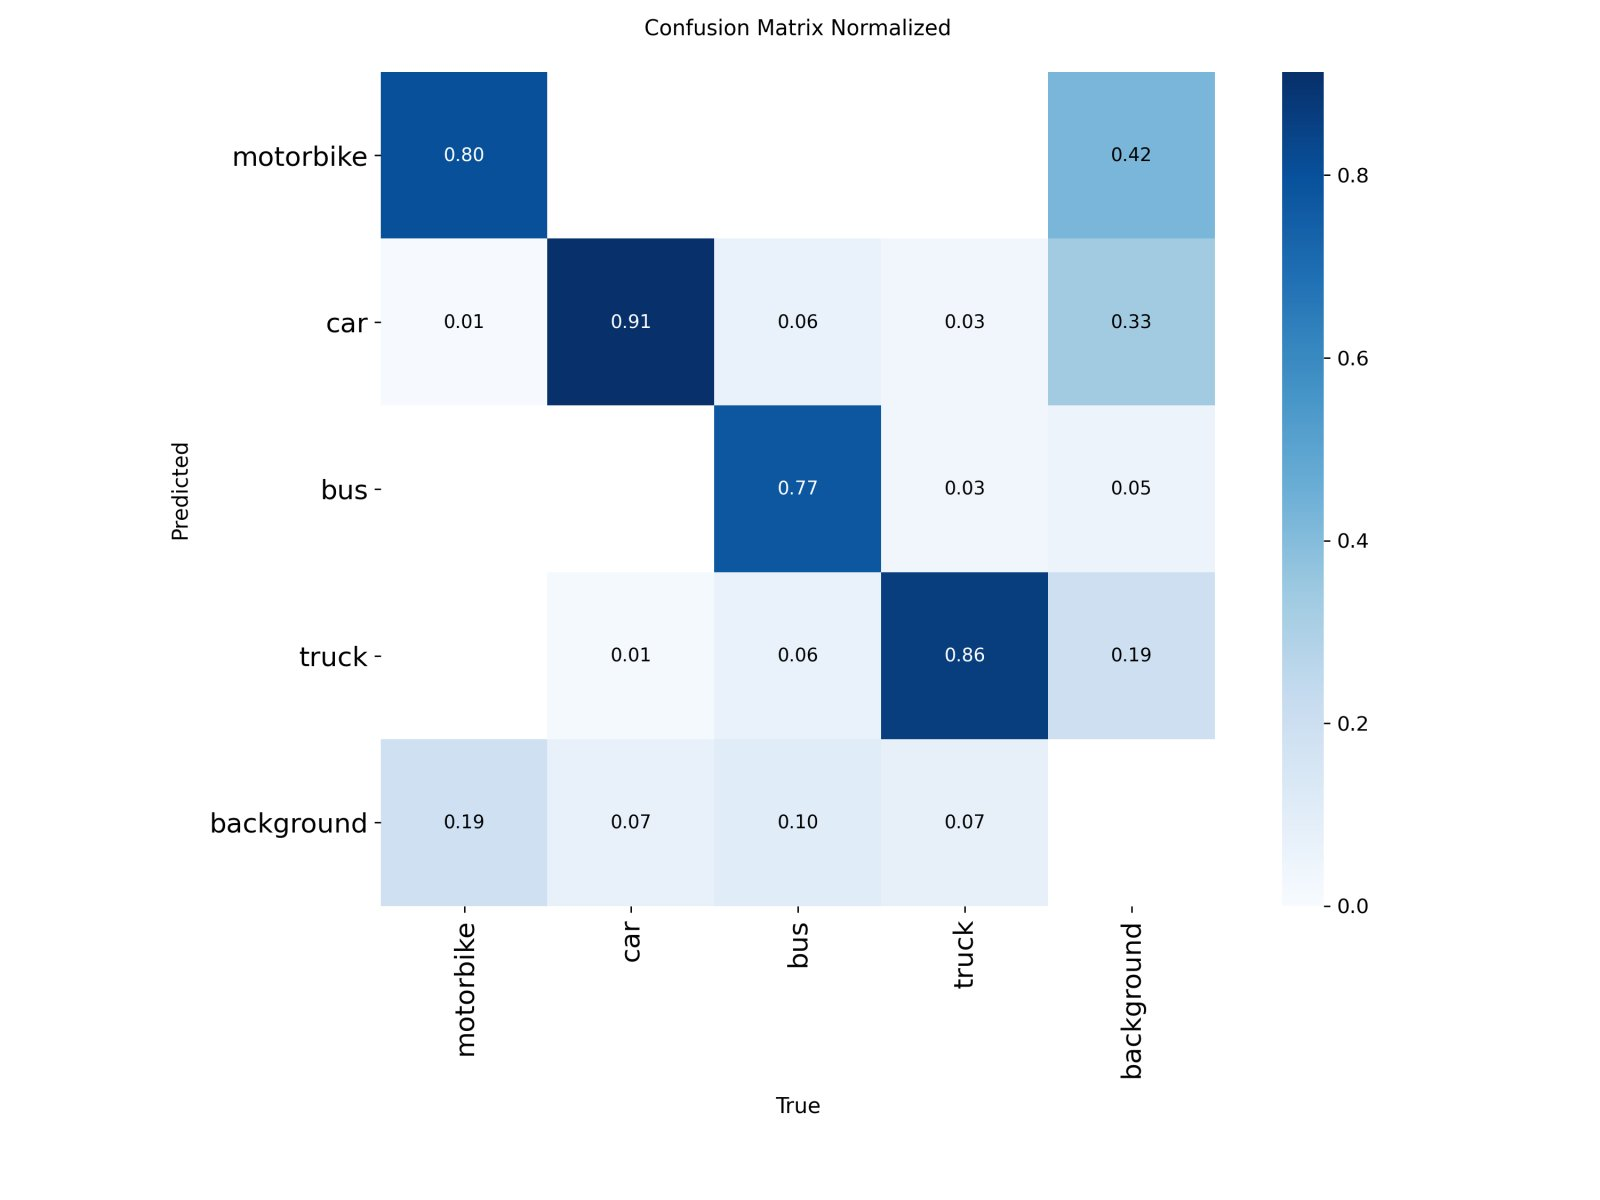
\includegraphics[width=0.72\linewidth]{v5_confusion_matrix.jpg}
  \caption{Ma trận nhầm lẫn chuẩn hoá của v5 trên tập test Roboflow (cột là lớp thật, hàng là lớp dự đoán)}
  \label{fig:confusion}
\end{figure}

\section{So sánh kiến trúc CNN và Transformer}
\label{sec:ket-qua-kien-truc}

Ba mô hình cùng dữ liệu v5, cùng giao thức (mục~\ref{sec:giao-thuc}), chấm một lần trên mọi tập.

\begin{table}[H]
  \centering
  \caption{mAP50 chính của ba kiến trúc và đối chứng cùng số điểm ảnh}
  \label{tab:kien-truc}
  \small
  \begin{tabularx}{\linewidth}{|p{3.4cm}|C|C|C|C|}
    \hline
    \thead{Tập} & \thead{YOLO26n (v5) @960} & \thead{YOLO26s @960} & \thead{RT-DETRv2-S @960×960} &
      \thead{YOLO26s @1280} \\ \hline
    Test Hà Nội & 0.923 & 0.914 & 0.929 & 0.915 \\ \hline
    \texttt{vn\_extra} ngày & 0.745 & 0.798 & \textbf{0.886} & 0.875 \\ \hline
    \texttt{vn\_extra} đêm & 0.628 & 0.713 & \textbf{0.816} & 0.800 \\ \hline
    20 frame PVD & 0.892 & 0.903 & 0.895 & 0.907 \\ \hline
    Test Roboflow (4 lớp) & 0.834 & 0.862 & 0.874 & -- \\ \hline
    Val UVH-26 (4 lớp) & 0.850 & 0.859 & \textbf{0.894} & 0.865 \\ \hline
    UA-DETRAC đêm & 0.845 & 0.876 & 0.887 & 0.862 \\ \hline
    UA-DETRAC ngày & 0.812 & 0.885 & 0.924 & 0.885 \\ \hline
  \end{tabularx}
\end{table}

\begin{table}[H]
  \centering
  \caption{mAP50-95 trên các tập có nhãn độc lập với mọi mô hình YOLO}
  \label{tab:kien-truc-5095}
  \small
  \begin{tabular}{|l|c|c|c|}
    \hline
    \thead{Tập} & \thead{YOLO26n (v5)} & \thead{YOLO26s} & \thead{RT-DETRv2-S} \\ \hline
    Val UVH-26 & 0.696 & 0.721 & \textbf{0.757} \\ \hline
    UA-DETRAC đêm & 0.538 & 0.554 & \textbf{0.588} \\ \hline
    UA-DETRAC ngày & 0.539 & 0.569 & \textbf{0.599} \\ \hline
  \end{tabular}
\end{table}

Từ Bảng~\ref{tab:kien-truc} và~\ref{tab:kien-truc-5095} rút ra ba kết luận:
\begin{enumerate}
  \item Cùng kích thước ảnh 960 (mặc định của mỗi họ), RT-DETRv2-S bằng hoặc hơn YOLO26s trên mọi tập. Chênh lệch rõ ở
        cảnh khó: \texttt{vn\_extra} ngày 0.886 so với 0.798, đêm 0.816 so với 0.713, val UVH-26 0.894 so với 0.859;
        hoà ở cảnh dễ (Hà Nội, PVD).
  \item Khi cho YOLO26s nhìn cùng số điểm ảnh (ảnh 1280), hai họ \textbf{hoà nhau} trên dữ liệu Việt Nam 1080p: khoảng tin
        cậy chồng nhau (ngày 0.875 [0.849--0.893] so với 0.886 [0.853--0.894]; đêm 0.800 [0.764--0.826] so với 0.816
        [0.782--0.840]), mAP50-95 ngày 0.588 so với 0.578, đêm 0.548 so với 0.547. Phần lớn lợi thế của RT-DETRv2 ở
        \texttt{vn\_extra} đến từ độ phân giải đầu vào chứ không phải từ kiến trúc.
  \item Trên hai tập có nhãn độc lập, RT-DETRv2-S có mAP50-95 cao hơn YOLO26s đều khoảng 0.03, tức box khít hơn. Ảnh
        UA-DETRAC chỉ 960×540 nên tăng ảnh lên 1280 không giúp YOLO (0.862 thấp hơn 0.876).
\end{enumerate}

YOLO26s hơn YOLO26n rõ ở \texttt{vn\_extra} và UA-DETRAC ngày, ngang nhau ở Hà Nội, PVD và UVH-26.
Hình~\ref{fig:acc-speed} đặt độ chính xác cạnh tốc độ CPU: mỗi bước tăng độ chính xác đều phải trả bằng thời gian xử
lý, và RT-DETRv2-S nằm xa nhất về phía chậm.

\begin{figure}[H]
  \centering
  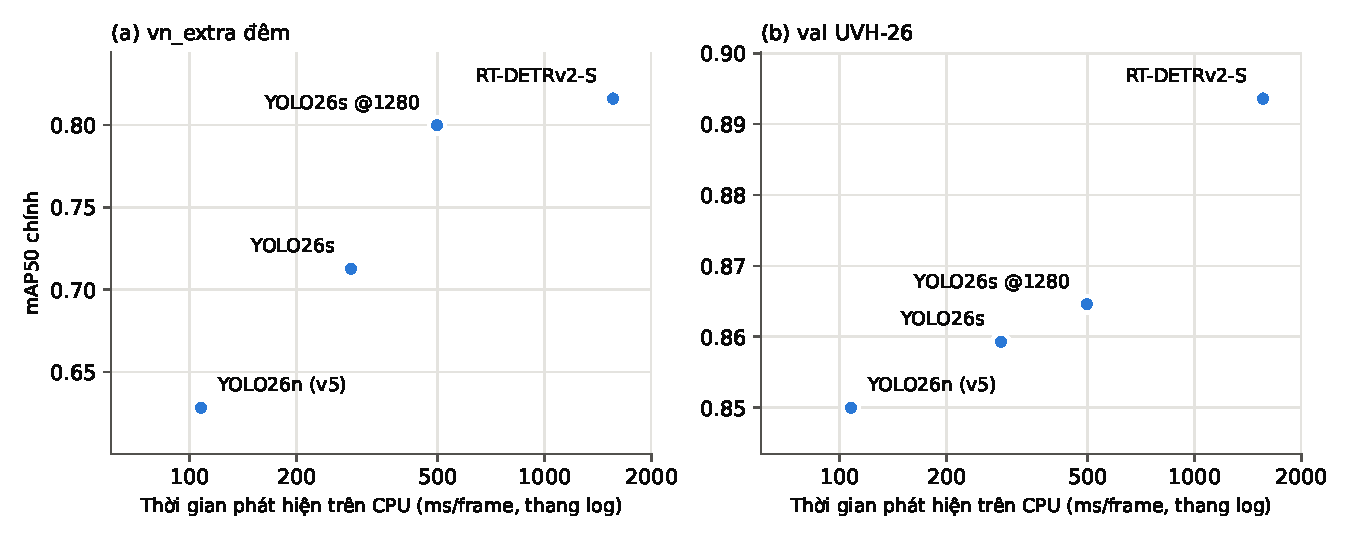
\includegraphics[width=\linewidth]{accuracy_vs_speed.pdf}
  \caption{Độ chính xác (mAP50 chính) theo thời gian phát hiện trên CPU i5-8250U của bốn cấu hình}
  \label{fig:acc-speed}
\end{figure}

\section{Tốc độ}
\label{sec:toc-do}

Laptop dòng U dễ bị hạ xung nhịp khi nóng, nên cách đo được thiết kế để công bằng giữa các mô hình: 5 đợt × 30 frame
video 1080p, các mô hình chạy xen kẽ trên cùng 30 frame và đảo thứ tự mỗi đợt, nghỉ giữa các đợt, khởi động mỗi mô hình
ít nhất 15 giây trước khi đo. ``Detector'' gồm tiền xử lý, suy luận và hậu xử lý; ``pipeline'' gồm cả đọc video và
theo dõi.

\begin{table}[H]
  \centering
  \caption{Tốc độ trên CPU Intel Core i5-8250U (ms/frame, trung vị [khoảng tứ phân vị])}
  \label{tab:toc-do-cpu}
  \footnotesize
  \begin{tabularx}{\linewidth}{|>{\raggedright\arraybackslash}p{2.2cm}|>{\centering\arraybackslash}p{1.55cm}|C|C|>{\centering\arraybackslash}p{1.15cm}|C|}
    \hline
    \thead{Mô hình} & \thead{Đầu vào} & \thead{Tham số / GFLOPs} & \thead{Detector} & \thead{frame/s} &
      \thead{Pipeline (frame/s)} \\ \hline
    YOLO26n v5, PyTorch & 544×960 & 2.51 M / 7.4 & 107.6 [92.0--129.3] & 9.3 & 206.4 (4.8) \\ \hline
    YOLO26n v5, OpenVINO & 544×960 & -- & 67.6 [64.7--74.1] & 14.8 & 155.7 (6.4) \\ \hline
    YOLO26s & 544×960 & 9.95 M / 28.7 & 284.8 [263.1--322.2] & 3.5 & 404.4 (2.5) \\ \hline
    YOLO26s @1280 & 736×1280 & 9.95 M / 52.4 & 497.3 [461.6--614.8] & 2.0 & 705.1 (1.4) \\ \hline
    RT-DETRv2-S & 960×960 & 20.08 M / 133.9 & 1561.0 [1441.7--1719.5] & 0.64 & -- \\ \hline
  \end{tabularx}
\end{table}

\begin{table}[H]
  \centering
  \caption{Tốc độ trên GPU Tesla T4 (Kaggle, PyTorch FP32; ms/frame và frame/s)}
  \label{tab:toc-do-gpu}
  \small
  \begin{tabular}{|l|c|c|}
    \hline
    \thead{Mô hình} & \thead{Detector} & \thead{Pipeline} \\ \hline
    YOLO26n v5 & 13.2 (75.7) & 23.7 (42.2) \\ \hline
    YOLO26s & 14.7 (68.0) & 23.5 (42.6) \\ \hline
    YOLO26s @1280 & 24.3 (41.2) & 33.2 (30.2) \\ \hline
    RT-DETRv2-S & 62.5 (16.0) & -- \\ \hline
  \end{tabular}
\end{table}

Trên CPU (Bảng~\ref{tab:toc-do-cpu}):
\begin{itemize}
  \item OpenVINO tăng tốc riêng phần phát hiện 1.6 lần (107.6 xuống 67.6 ms) nhưng cả pipeline chỉ 1.3 lần, vì pipeline
        còn tốn khoảng 90--100 ms mỗi frame cho giải mã video 1080p và tracker (lúc đo vẫn bật GMC). Trong một phép đo
        riêng cùng điều kiện, tắt GMC giảm thời gian pipeline OpenVINO từ 128 xuống 92 ms (7.8 lên 10.8 frame/s).
  \item RT-DETRv2-S mất 1.56 giây mỗi frame: chậm hơn YOLO26s ở ảnh 960 khoảng 5.5 lần, hơn YOLO26s ở ảnh 1280 (độ chính
        xác ngang nhau trên dữ liệu Việt Nam) 3.1 lần, hơn v5 14 lần và hơn v5 OpenVINO 23 lần. Mô hình này không dùng
        được cho video trên CPU.
\end{itemize}

Trên GPU (Bảng~\ref{tab:toc-do-gpu}), YOLO26n và YOLO26s gần như nhanh bằng nhau (cả pipeline khoảng 42 frame/s): mô
hình nhỏ không tận dụng hết GPU, phần thời gian còn lại là tiền xử lý, hậu xử lý và tracker chạy trên CPU. Vì vậy nếu có
GPU nên dùng YOLO26s, chính xác hơn ở cảnh khó mà không chậm hơn. RT-DETRv2-S trên GPU vẫn chậm hơn YOLO26s khoảng 4
lần nhưng đạt 16 frame/s cho riêng phần phát hiện.

\section{Kết quả theo dõi}
\label{sec:theo-doi}

\subsection{Tập dev VnTraffic}

\begin{table}[H]
  \centering
  \caption{So sánh ba thuật toán theo dõi trên VnTraffic (mô hình v3, tham số mặc định)}
  \label{tab:tracker}
  \small
  \begin{tabular}{|l|c|c|c|c|c|c|}
    \hline
    \thead{Tracker} & \thead{HOTA} & \thead{AssA} & \thead{IDR} & \thead{Đổi ID} & \thead{MOTA} & \thead{frame/s CPU} \\ \hline
    ByteTrack & 0.480 & 0.615 & 0.708 & 147 & 0.054 & 4.4 \\ \hline
    \textbf{BoT-SORT} & 0.505 & \textbf{0.659} & \textbf{0.738} & \textbf{128} & 0.068 & 3.6 \\ \hline
    OC-SORT & 0.493 & 0.594 & 0.669 & 206 & 0.227 & 4.0 \\ \hline
  \end{tabular}
\end{table}

BoT-SORT tốt nhất trên cả ba chỉ số không phụ thuộc phát hiện thừa (Bảng~\ref{tab:tracker}). MOTA ở đây rất thấp và
không dùng để kết luận: khoảng 21 box mỗi frame của tracker không khớp nhãn, phần lớn là xe máy thật trong cụm dày mà
nhãn bỏ sót. OC-SORT có MOTA cao hơn chỉ vì xuất ít box hơn.

Chỉnh lưới 18 cấu hình BoT-SORT và ByteTrack: giữ track mất 90 frame, không ReID cho IDR 0.744 và AssA 0.668 (mặc định:
0.738 và 0.659), số lần đổi ID không đổi (128). Bật ReID làm số lần đổi ID tăng lên 207--211. Lọc track dưới 3 frame giảm
đổi ID từ 128 xuống 118, IDR giảm 0.004.

\begin{table}[H]
  \centering
  \caption{Ảnh hưởng của mô hình phát hiện lên theo dõi trên VnTraffic (cùng BoT-SORT đã chỉnh)}
  \label{tab:detector-tracking}
  \small
  \begin{tabular}{|l|c|c|c|c|c|c|}
    \hline
    \thead{Detector} & \thead{HOTA} & \thead{AssA} & \thead{IDR} & \thead{Đổi ID} & \thead{FN} & \thead{Số track} \\ \hline
    v3 & 0.507 & 0.668 & 0.744 & 128 & 2.550 & 467 \\ \hline
    v4 @1280 & 0.555 & 0.684 & 0.738 & 91 & 2.697 & 344 \\ \hline
    \textbf{v5} & 0.554 & \textbf{0.709} & \textbf{0.827} & \textbf{62} & \textbf{1.058} & 334 \\ \hline
    v5 @1280 & 0.549 & 0.713 & 0.820 & 85 & 1.183 & 341 \\ \hline
  \end{tabular}
\end{table}

Đổi từ v3 sang v5 là cải tiến lớn nhất cho theo dõi (Bảng~\ref{tab:detector-tracking}): số box bỏ sót giảm hơn một nửa
(2.550 xuống 1.058), IDR tăng từ 0.744 lên 0.827, số lần đổi ID giảm từ 128 xuống 62. Soi từng xe, các xe v3 bỏ sót
như một xe buýt (điểm tin cậy 0 lên 0.84--0.87 với v5), một xe tải (dưới 0.14 lên 0.93--0.94) và một xe máy đang dừng
(0.01--0.12 lên 0.52--0.82) đều được v5 nhận ra. Phát hiện ổn định thì quỹ đạo ít bị đứt. Tắt GMC cho kết quả gần như
y hệt (IDR 0.827 cả hai bản, đổi ID 61 so với 62).

\subsection{Tập test clip Phạm Văn Đồng}

\begin{table}[H]
  \centering
  \caption{Kết quả theo dõi trên tập test (clip Phạm Văn Đồng 20 giây, 183 quỹ đạo nhãn)}
  \label{tab:tracking-test}
  \footnotesize
  \begin{tabularx}{\linewidth}{|L|c|c|c|c|c|c|c|c|}
    \hline
    \thead{Cấu hình} & \thead{HOTA} & \thead{DetA} & \thead{AssA} & \thead{MOTA} & \thead{IDF1} & \thead{IDR} & \thead{IDP} &
      \thead{Đổi ID} \\ \hline
    v5 + BoT-SORT đã chỉnh, không GMC (mặc định) & 0.718 & 0.670 & 0.784 & 0.813 & 0.880 & 0.822 & 0.947 & 26 \\ \hline
    v5 + BoT-SORT đã chỉnh, có GMC & 0.718 & 0.672 & 0.783 & 0.815 & 0.880 & 0.822 & 0.946 & 28 \\ \hline
  \end{tabularx}
\end{table}

Trên tập test có nhãn đầy đủ, cấu hình mặc định đạt HOTA 0.718, MOTA 0.813, IDF1 0.880, đổi ID 26 lần trên 183 xe
(Bảng~\ref{tab:tracking-test}). IDP 0.947 cao hơn IDR 0.822: hệ thống ít khi gán nhầm danh tính, phần mất chủ yếu
do bỏ sót (2.157 box bỏ sót so với 357 box thừa).

\begin{table}[H]
  \centering
  \caption{Ablation trên tập test (chỉ để báo cáo, lựa chọn đã chốt trên dev)}
  \label{tab:ablation}
  \small
  \begin{tabular}{|l|c|c|c|c|}
    \hline
    \thead{Detector + tracker} & \thead{HOTA} & \thead{MOTA} & \thead{IDF1} & \thead{Đổi ID} \\ \hline
    v5 + BoT-SORT & 0.718 & 0.815 & 0.880 & 28 \\ \hline
    v5 + ByteTrack & 0.698 & 0.791 & 0.872 & 34 \\ \hline
    v5 + OC-SORT & 0.692 & 0.786 & 0.865 & 56 \\ \hline
    v3 + BoT-SORT đã chỉnh & 0.741 & 0.763 & 0.845 & 44 \\ \hline
  \end{tabular}
\end{table}

Bảng~\ref{tab:ablation} xác nhận lựa chọn trên dev: với cùng v5, BoT-SORT tốt nhất trên test. So v5 với v3, v5 hơn rõ ở
MOTA (0.815 so với 0.763), IDF1 (0.880 so với 0.845) và số lần đổi ID (28 so với 44). HOTA trung bình của v3 cao hơn
(0.741 so với 0.718) nhưng đây là thiên lệch do nhãn sơ bộ, phân tích ở mục~\ref{sec:thao-luan}. Lọc track dưới 3 frame
giảm đổi ID của v5 từ 28 xuống 23, HOTA giảm nhẹ từ 0.718 xuống 0.708.

\section{Sai số đếm xe qua vạch}
\label{sec:dem-xe}

Số lượt xe thật được tính bằng cách cho các quỹ đạo nhãn tay của clip test đi qua đúng bộ đếm của hệ thống, nên chênh
lệch chỉ do phát hiện và theo dõi. Vạch đếm là vạch mặc định của hệ thống (nằm ngang ở 60\% chiều cao ảnh), không chọn
theo kết quả.

\begin{table}[H]
  \centering
  \caption{Số lượt xe qua vạch trên clip test 20 giây: nhãn tay và hệ thống}
  \label{tab:dem-xe}
  \small
  \begin{tabular}{|l|c|c|c|c|c|c|c|}
    \hline
    \thead{Lớp} & \thead{Thật vào} & \thead{Thật ra} & \thead{Đếm vào} & \thead{Đếm ra} & \thead{Thật tổng} &
      \thead{Đếm tổng} & \thead{Sai số} \\ \hline
    Xe máy & 1 & 52 & 0 & 53 & 53 & 53 & 2 \\ \hline
    Ô tô & 1 & 18 & 0 & 19 & 19 & 19 & 2 \\ \hline
    Xe buýt & 0 & 1 & 0 & 0 & 1 & 0 & 1 \\ \hline
    Xe tải & 0 & 0 & 0 & 0 & 0 & 0 & 0 \\ \hline
    \textbf{Tổng} & 2 & 71 & 0 & 72 & 73 & 72 & 3 (4.1\%) \\ \hline
  \end{tabular}
\end{table}

Hệ thống đếm 72 lượt so với 73 lượt thật (Bảng~\ref{tab:dem-xe}); tổng theo lớp khớp hoàn toàn ở xe máy (53) và ô tô
(19). Sai số tính theo từng hướng là 3 lượt. Xem lại từng lượt:
\begin{itemize}
  \item Hai lượt ``vào'' của nhãn (một ô tô, một xe máy) là hiện tượng của nhãn ở tán cây: xe khuất dần sau cây, box nhãn
        chỉ ôm phần nhìn thấy nên cạnh đáy box đi ngược lên qua vạch, dù xe không đi ngược chiều. Vạch y = 0.6 đi qua mép
        tán cây bên phải.
  \item Lượt xe buýt là một chiếc Ford Transit bị đếm thành ô tô, đúng vấn đề định nghĩa lớp van đã nêu.
\end{itemize}

Như vậy lỗi thật của hệ thống trên clip này là 1 lượt sai lớp; không có xe bị sót hay bị đếm trùng. Khi triển khai, nên
đặt vạch đếm ở vùng không bị che.

\section{Kết quả ở cảnh ban đêm}

Ba nguồn bằng chứng về cảnh đêm cho cùng một hướng:
\begin{itemize}
  \item \textbf{\texttt{vn\_extra} đêm} (cảnh đêm Việt Nam có nhãn): v5 đạt 0.628, cao hơn v3 (0.437) và mô hình gốc
        COCO (0.437); YOLO26s đạt 0.713, RT-DETRv2-S 0.816.
  \item \textbf{UA-DETRAC}: cả ba mô hình COCO, v3, v5 không giảm độ chính xác khi trời tối (v5: đêm 0.845, ngày
        0.812). Tuy vậy đêm của UA-DETRAC là đường phố có đèn, chủ yếu ô tô, khác đường tối ở hầm chui.
  \item \textbf{Ba clip hầm chui không có nhãn}, dùng chỉ số thay thế trên 20 giây mỗi clip với mốc ban ngày là clip
        Phạm Văn Đồng: độ tin cậy trung vị của v5 là 0.59--0.63 ban đêm so với 0.63 ban ngày, tỉ lệ track ngắn dưới 1
        giây 47--52\% so với 54\%, tức v5 gần như không suy giảm; v3 tụt rõ (độ tin cậy 0.36--0.45, 67--73\% track
        ngắn). Đây là chỉ số thay thế, chỉ dùng để so tương đối.
\end{itemize}

\section{Phân tích lỗi}
\label{sec:phan-tich-loi}

Các ảnh dưới đây được chọn bằng cách đếm lỗi của v5 (ngưỡng tin cậy 0.25, ghép IoU 0.5) trên các tập test và lấy ảnh có
nhiều lỗi loại đó nhất. Màu box: xanh lá là đúng, đỏ là bỏ sót, cam là sai lớp, tím là thừa, xám là vùng bỏ qua. Ảnh chỉ
để minh hoạ; số lượng lỗi định lượng nằm ở các bảng phía trên.

\begin{figure}[H]
  \centering
  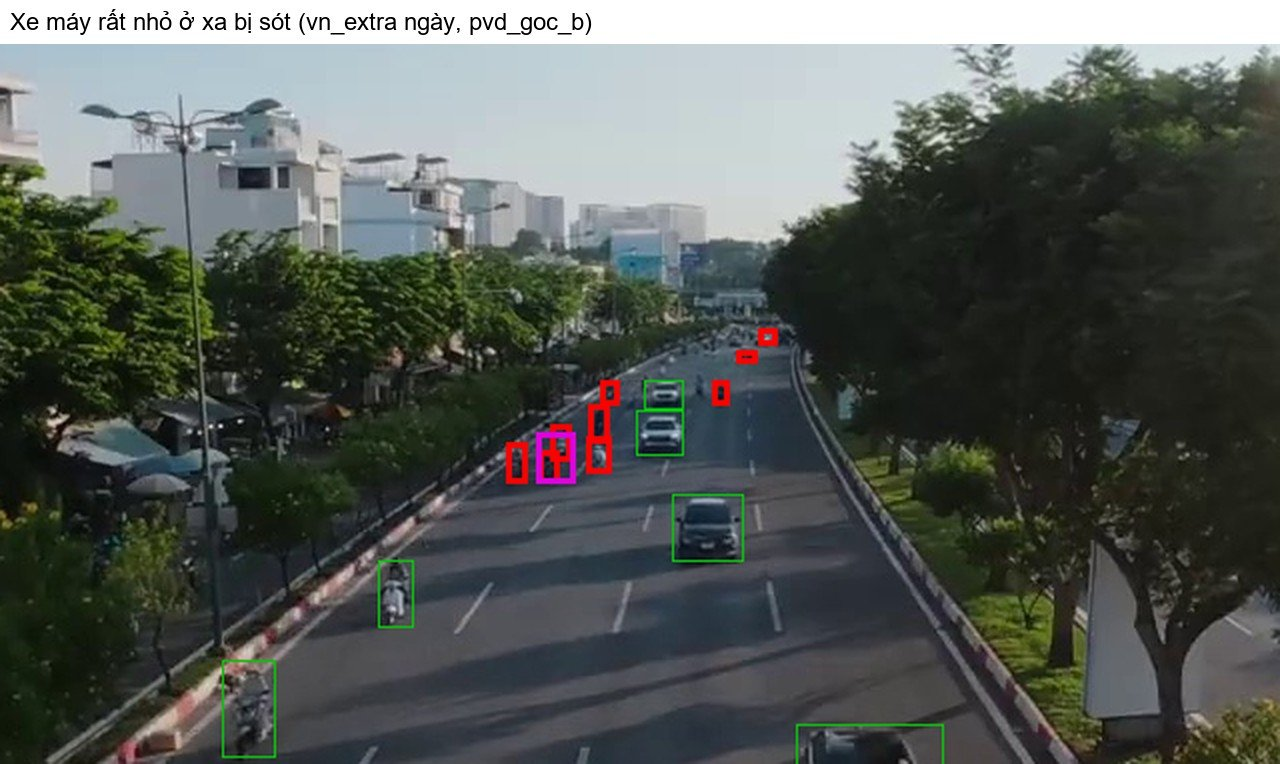
\includegraphics[width=0.9\linewidth]{error_1.jpg}
  \caption{Lỗi 1: xe máy rất nhỏ ở xa bị bỏ sót (\texttt{vn\_extra} ngày, góc máy B)}
  \label{fig:error-1}
\end{figure}

\begin{figure}[H]
  \centering
  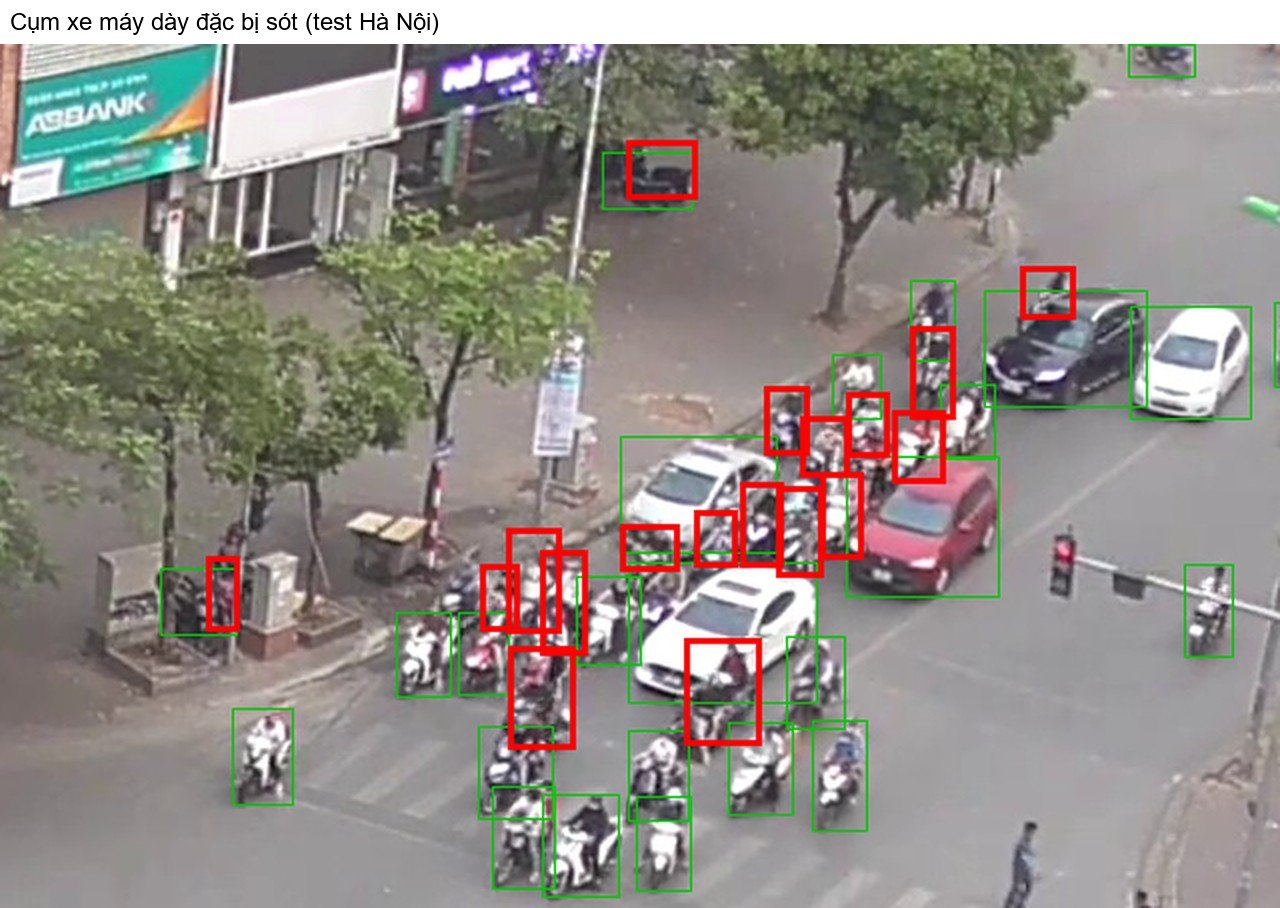
\includegraphics[width=0.9\linewidth]{error_2.jpg}
  \caption{Lỗi 2: cụm xe máy chờ đèn đỏ dày đặc bị bỏ sót (test Hà Nội)}
  \label{fig:error-2}
\end{figure}

Lỗi 1 và 2 (Hình~\ref{fig:error-1}, \ref{fig:error-2}) là hai dạng bỏ sót chính ban ngày: xe quá nhỏ sau khi ảnh bị thu
về 960 điểm ảnh, và xe máy dừng sát nhau che khuất lẫn nhau.

\begin{figure}[H]
  \centering
  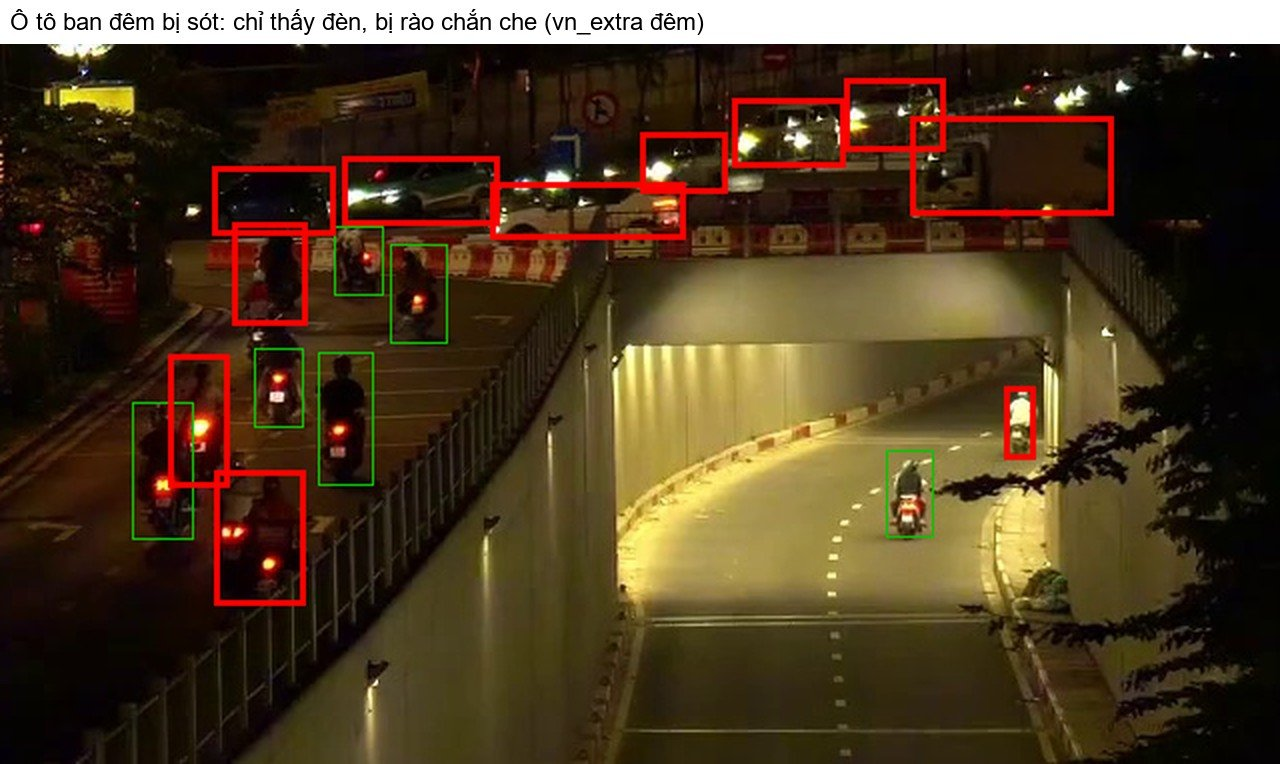
\includegraphics[width=0.9\linewidth]{error_3.jpg}
  \caption{Lỗi 3: ô tô ban đêm ở đường ngang phía xa bị rào chắn che, chỉ thấy đèn (\texttt{vn\_extra} đêm)}
  \label{fig:error-3}
\end{figure}

\begin{figure}[H]
  \centering
  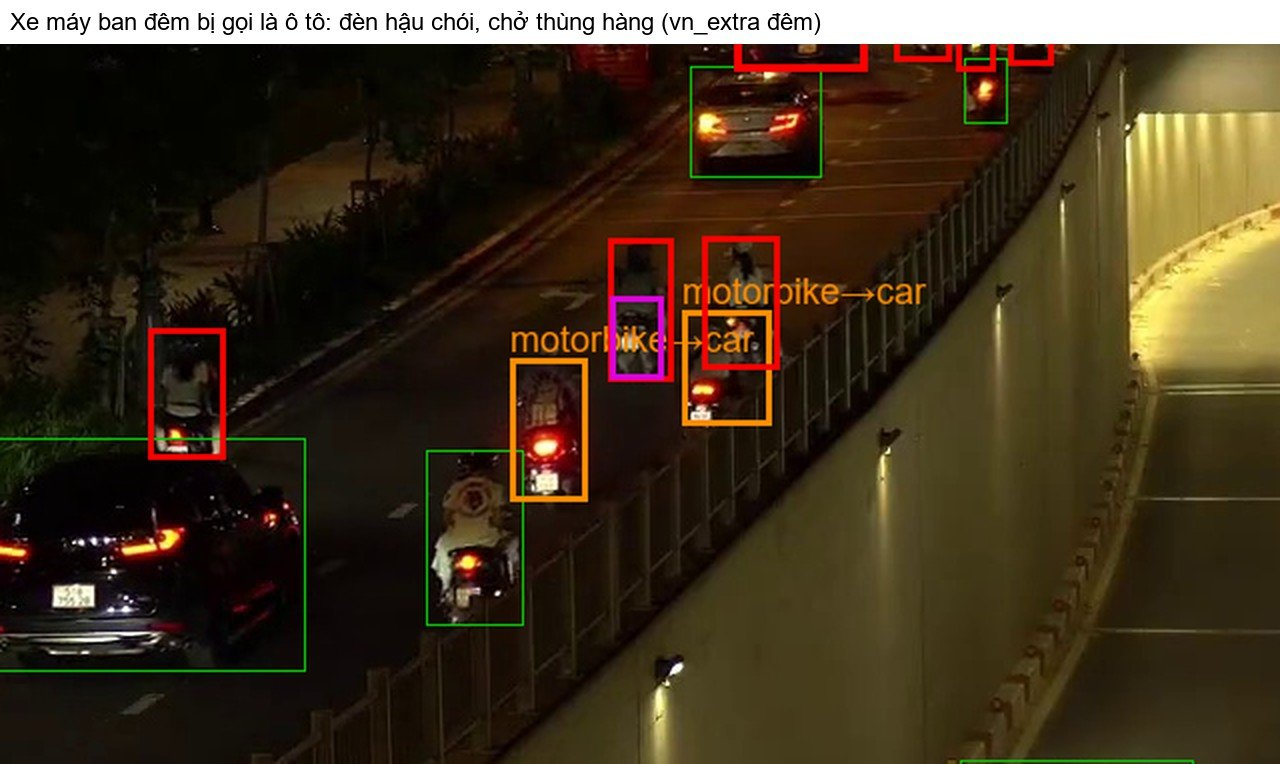
\includegraphics[width=0.9\linewidth]{error_4.jpg}
  \caption{Lỗi 4: xe máy ban đêm bị gọi là ô tô do đèn hậu chói, xe chở thùng hàng (\texttt{vn\_extra} đêm)}
  \label{fig:error-4}
\end{figure}

\begin{figure}[H]
  \centering
  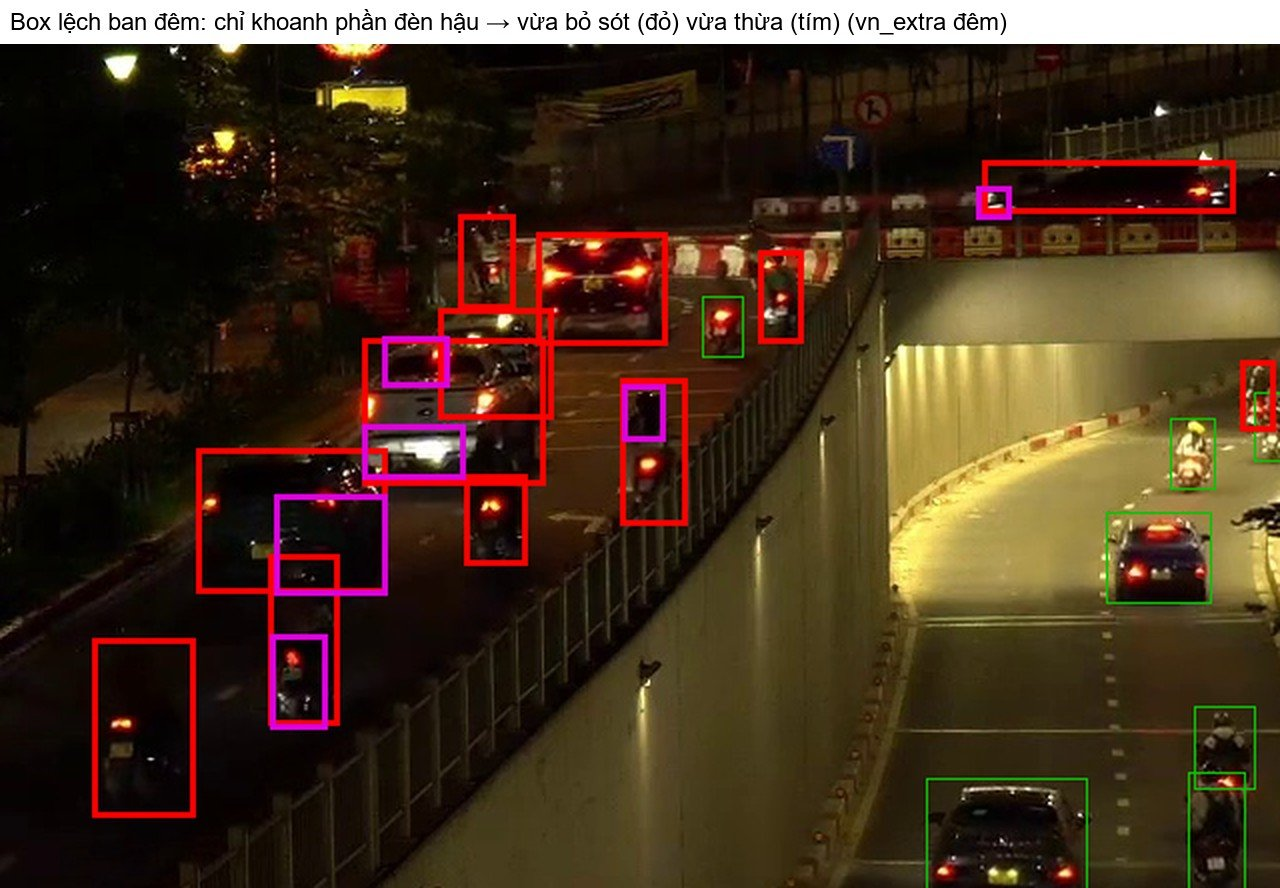
\includegraphics[width=0.9\linewidth]{error_5.jpg}
  \caption{Lỗi 5: box lệch ban đêm, mô hình chỉ khoanh phần đèn hậu sáng nên một xe bị tính cả bỏ sót (đỏ) lẫn thừa
           (tím) (\texttt{vn\_extra} đêm)}
  \label{fig:error-5}
\end{figure}

Ở cảnh đêm (Hình~\ref{fig:error-3}--\ref{fig:error-5}), ngoài xe chỉ thấy đèn bị sót, có hai lỗi đặc trưng. Xe máy chở
hàng có đèn chói bị gọi là ô tô. Và mô hình hay chỉ khoanh phần đèn hậu sáng: box này có IoU dưới 0.5 với box nhãn (bao
cả người và xe), nên một xe vừa bị tính là bỏ sót vừa sinh một phát hiện thừa. Phần lớn ``phát hiện thừa'' ban đêm thuộc
loại này chứ không phải vệt đèn hay bóng phản chiếu.

\begin{figure}[H]
  \centering
  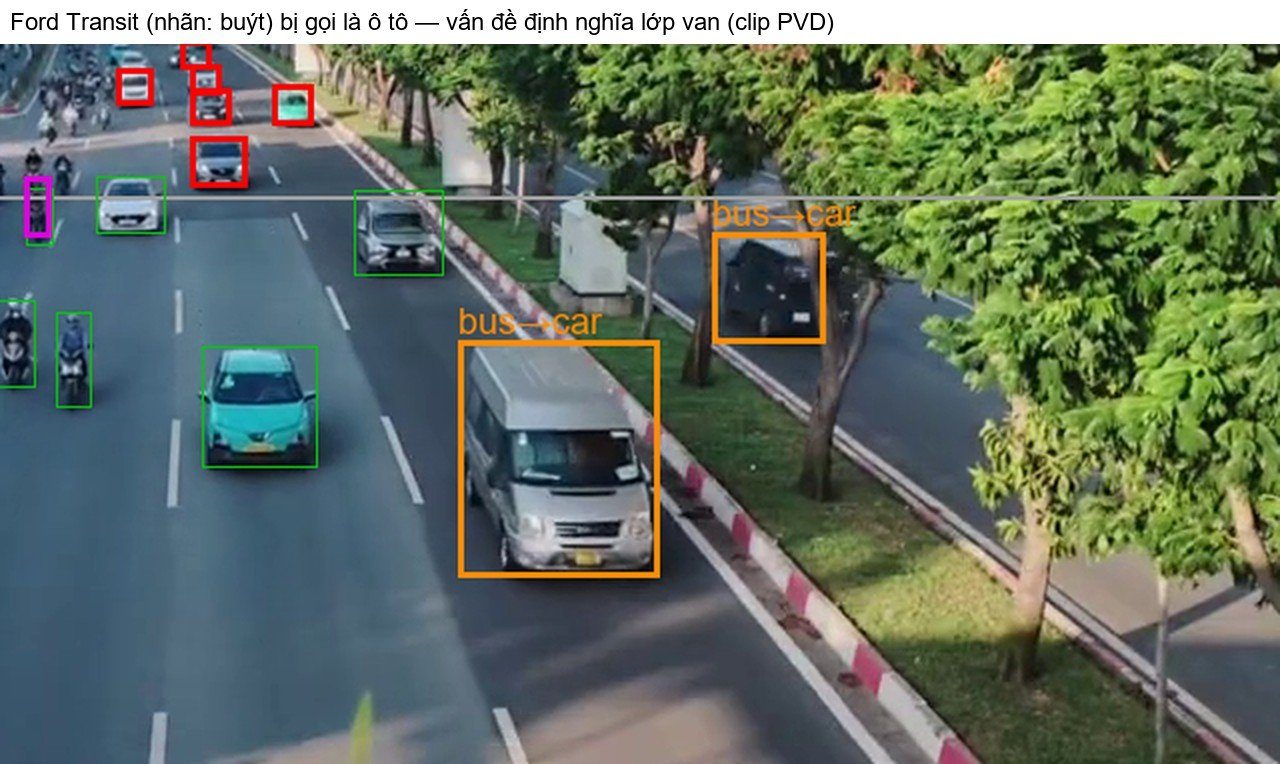
\includegraphics[width=0.9\linewidth]{error_6.jpg}
  \caption{Lỗi 6: xe Ford Transit (nhãn xe buýt) bị gọi là ô tô (clip Phạm Văn Đồng)}
  \label{fig:error-6}
\end{figure}

\begin{figure}[H]
  \centering
  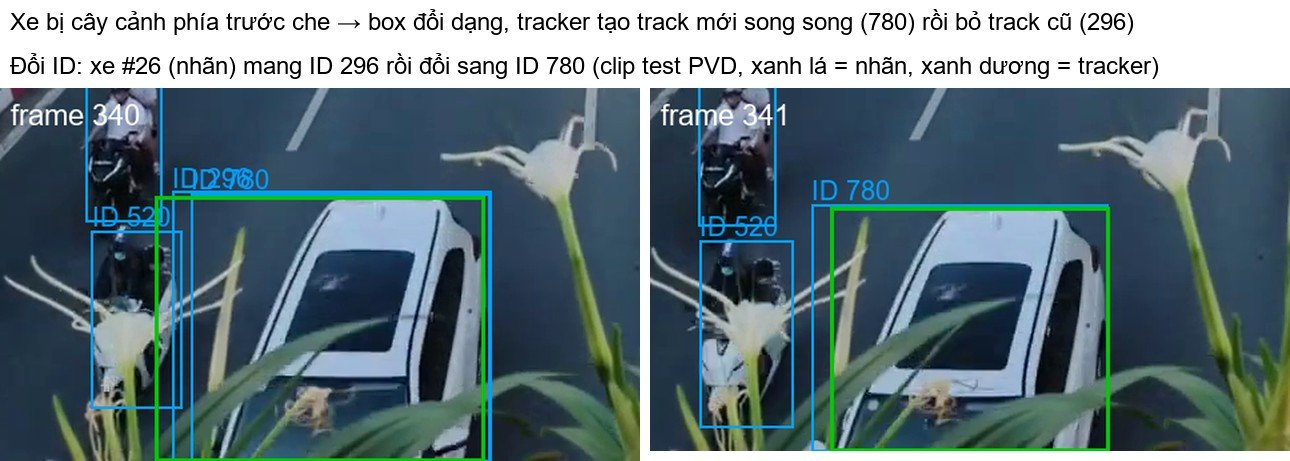
\includegraphics[width=\linewidth]{error_7.jpg}
  \caption{Lỗi 7: đổi ID khi xe bị cây cảnh phía trước che; box đổi dạng, tracker tạo track mới song song rồi bỏ track
           cũ (clip Phạm Văn Đồng)}
  \label{fig:error-7}
\end{figure}

Lỗi 6 (Hình~\ref{fig:error-6}) là hệ quả của định nghĩa lớp xe van. Lỗi 7 (Hình~\ref{fig:error-7}) là dạng đổi ID điển
hình: khi xe đi sau cây, box co lại theo phần nhìn thấy, tracker không ghép được với track cũ nên tạo track mới. Bộ dò
đổi ID đơn giản của đề tài (ghép IoU từng frame) đếm được 46 lần; lọc thêm điều kiện ``ID cũ đã biến mất ở frame đổi''
còn 25 lần, gần với 26 lần đổi ID của TrackEval. Phần chênh lệch là box của tracker nhảy qua lại giữa hai track trùng
trên cùng một xe.

\section{Ứng dụng web và video demo}

Web demo (Hình~\ref{fig:app}) cho chọn clip, xem video kết quả có box, ID, vết di chuyển và vạch đếm, cùng bảng đếm
theo lớp và hướng, biểu đồ số xe cộng dồn theo thời gian, danh sách sự kiện và nút tải CSV. Chế độ mặc định nạp video
đã xử lý sẵn trên GPU để trình chiếu mượt; chế độ chạy trực tiếp trên CPU dùng khi cần xử lý video mới.

\begin{figure}[H]
  \centering
  \begin{subfigure}{\linewidth}
    \centering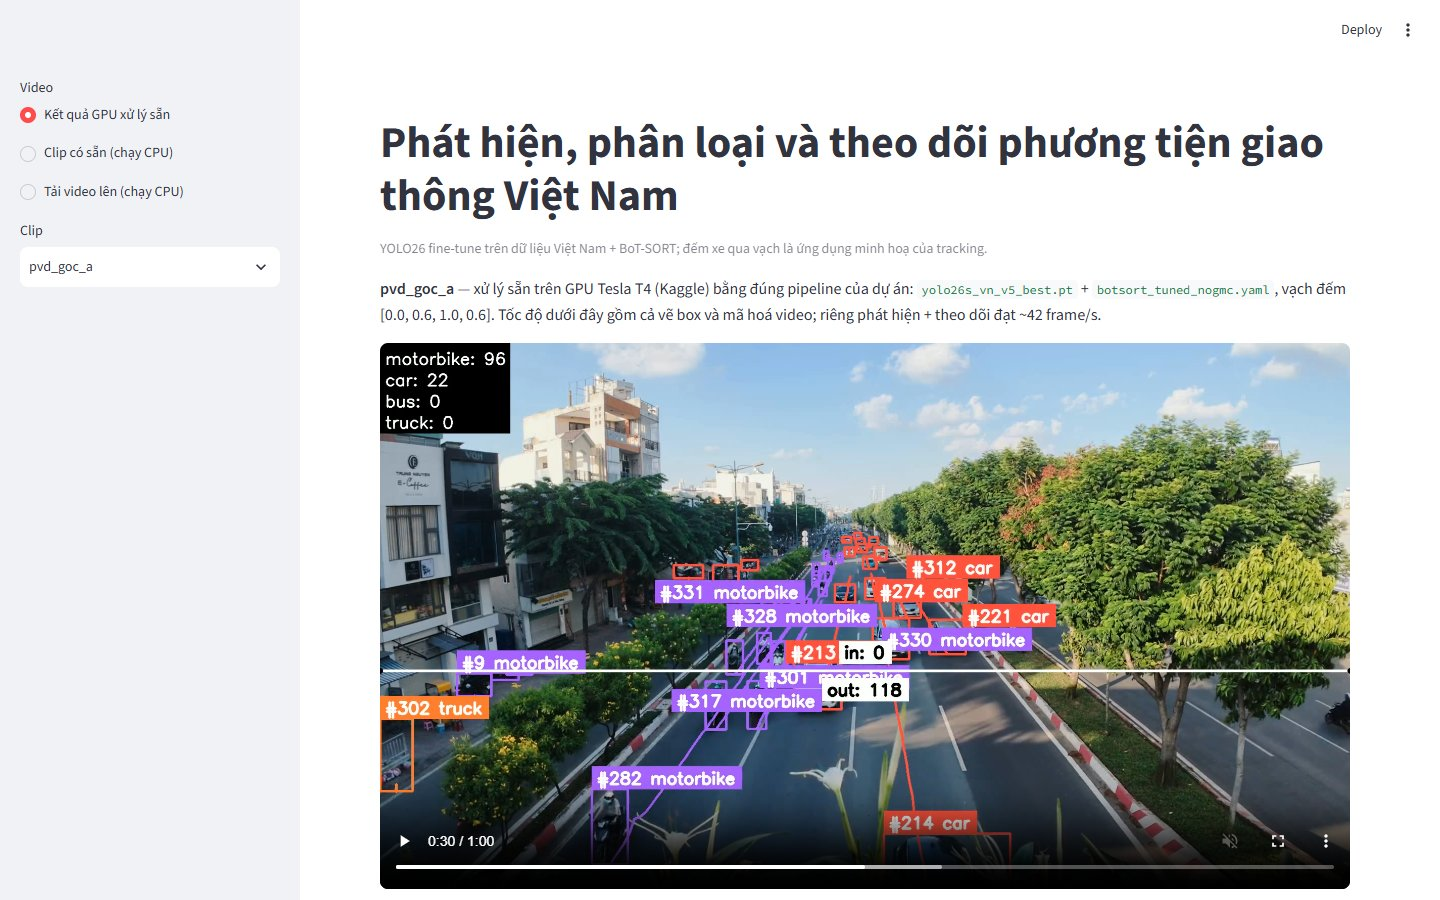
\includegraphics[width=0.92\linewidth]{app_gpu_demo.jpg}
    \caption{Video kết quả của clip Phạm Văn Đồng}
  \end{subfigure}\\[6pt]
  \begin{subfigure}{\linewidth}
    \centering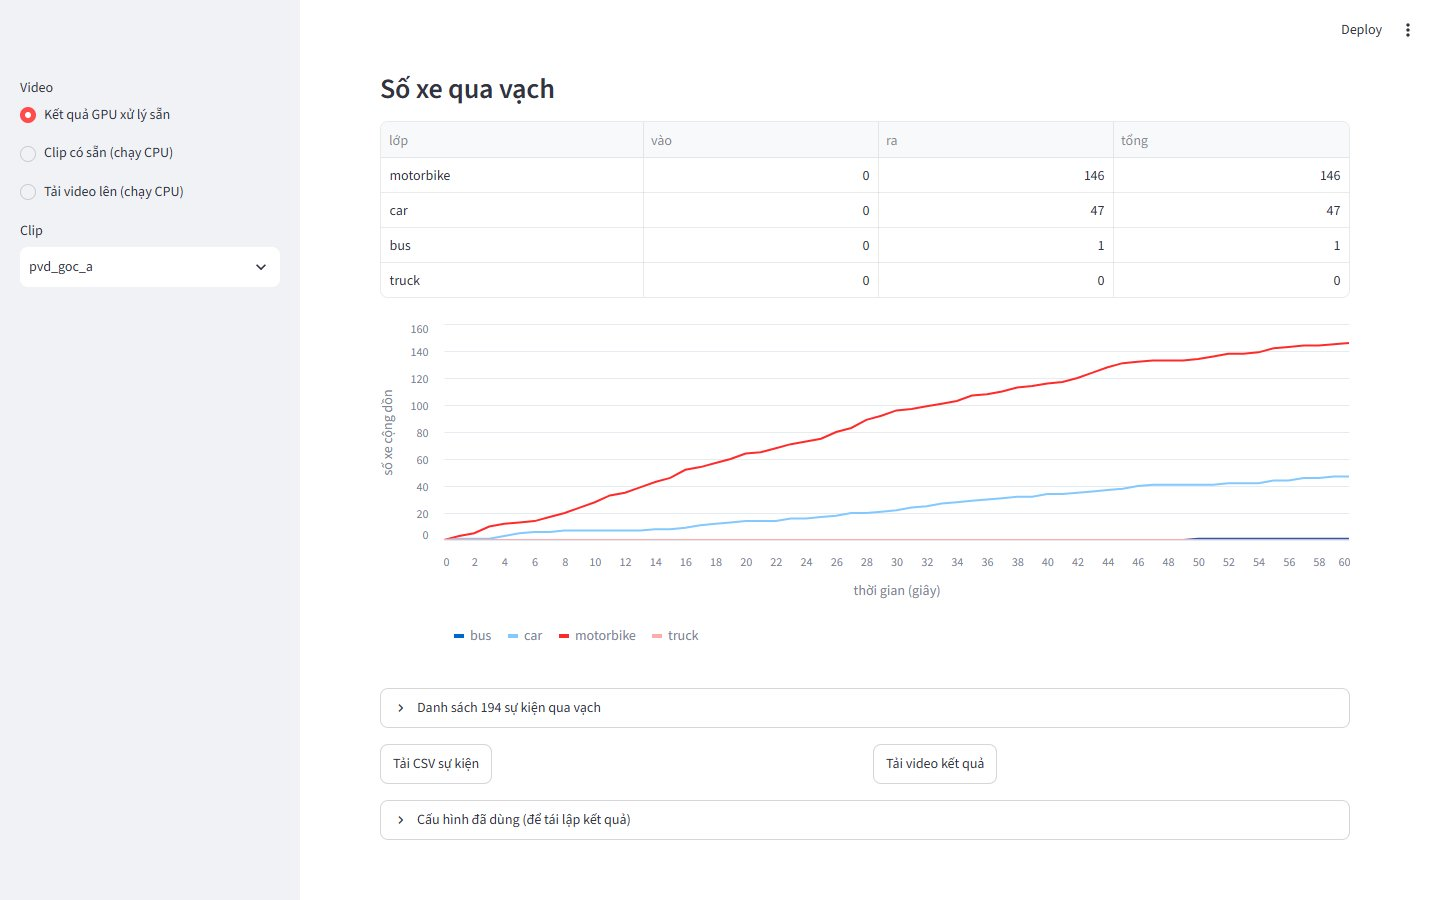
\includegraphics[width=0.92\linewidth]{app_counts.jpg}
    \caption{Bảng đếm theo lớp và hướng, biểu đồ số xe cộng dồn}
  \end{subfigure}
  \caption{Giao diện web demo Streamlit}
  \label{fig:app}
\end{figure}

Sáu clip demo dài 60 giây (ba góc máy đại lộ Phạm Văn Đồng và ba đoạn hầm chui ban đêm) được xử lý sẵn trên GPU T4 bằng
YOLO26s ở ảnh 960 và BoT-SORT đã chỉnh, đúng chương trình dùng trên máy local. Tính cả vẽ kết quả và mã hoá video 1080p,
tốc độ xử lý là 15.4--20.9 frame/s; con số này thấp hơn khoảng 42 frame/s của riêng phát hiện và theo dõi, vì khi có
GPU thì việc vẽ và ghi video trên CPU trở thành phần chậm nhất. Số lượt qua vạch trong 60 giây: góc A 194 (chỉ chiều ra,
vì làn ngược chiều ra khỏi khung hình trước vạch), góc B 169, góc C 254; ba đoạn hầm chui 69, 76 và 98. Các clip này
chưa có nhãn nên những con số này không phải số đánh giá. Hình~\ref{fig:demo-dem} là một frame của clip ban đêm.

\begin{figure}[H]
  \centering
  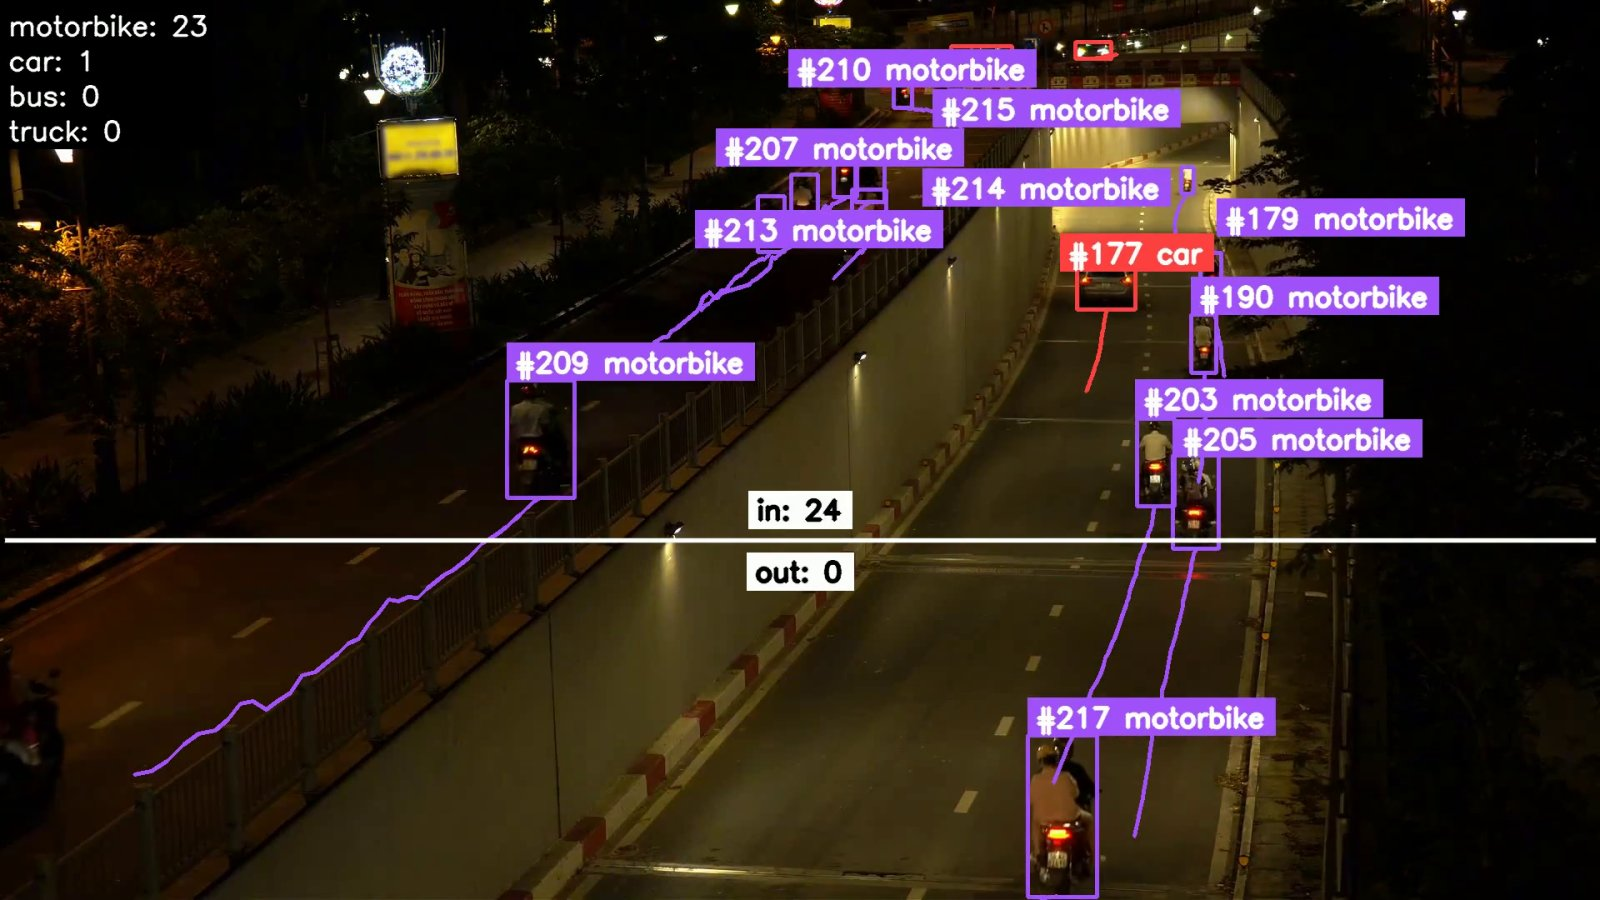
\includegraphics[width=0.92\linewidth]{demo_ham_chui_dem_1.jpg}
  \caption{Frame video demo ban đêm ở lối vào hầm chui TP.HCM (nguồn video: kênh YouTube Midnight Soundscape)}
  \label{fig:demo-dem}
\end{figure}

\section{Nhận xét và thảo luận}
\label{sec:thao-luan}

\textbf{Thiên lệch do nhãn sơ bộ.} Nhãn tay của đề tài đều được sửa từ nhãn sơ bộ của một mô hình, và box người gán giữ
nguyên mang cách khoanh box của mô hình đó. Ở test Hà Nội, 69\% box là box sơ bộ của v2 giữ nguyên, nên mAP50-95 thiên vị
mạnh v2: v2 đạt 0.815 trong khi v3 chỉ 0.765, ngược với mọi chỉ số khác. Clip Phạm Văn Đồng có nhãn sơ bộ từ v3, nên
HOTA của v3 cao hơn v5 chỉ ở các ngưỡng IoU chặt: ở IoU 0.5 HOTA của v5 là 0.844 so với 0.825 của v3, còn ở IoU 0.9 là
0.295 so với 0.412. Trên test Hà Nội (nhãn sơ bộ từ v2, không phải v3), mAP50-95 của v5 và v3 bằng nhau. Vì vậy trên các
tập này đề tài chỉ dùng mAP50 và các chỉ số theo dõi ở ngưỡng mặc định; so box khít (mAP50-95) chỉ trên tập có nhãn độc
lập. Tập \texttt{vn\_extra} được làm sau khi nhận ra vấn đề này, với nhãn sơ bộ từ một mô hình không tham gia so sánh.

\textbf{Vì sao chọn v5 và BoT-SORT.} Trên tập phát hiện Hà Nội, v3, v4, v5 hoà nhau; v5 được chọn vì tác động lên theo
dõi (đổi ID giảm một nửa trên dev) và vì tốt hơn rõ ở cảnh đêm, UVH-26 và UA-DETRAC. Điều này cho thấy dữ liệu đúng góc
camera giao thông quan trọng hơn kích thước ảnh: v4 (ảnh 1280) chỉ sửa được 1/4 số frame xe máy từng bị sót, còn v5 ở
ảnh 960 nhận ra được phần lớn các trường hợp đó. Ngoại lệ là cảnh có nhiều xe rất nhỏ ở xa, nơi ảnh 1280 có lợi rõ.

\textbf{Đánh đổi độ chính xác và tốc độ.} RT-DETRv2-S chính xác nhất và cho box khít nhất, nhưng chậm 23 lần so với v5
OpenVINO trên CPU. Khi cho YOLO cùng số điểm ảnh, khoảng cách độ chính xác trên dữ liệu Việt Nam gần như biến mất. Vì vậy
mô hình triển khai là v5 (OpenVINO) trên CPU; nếu có GPU thì dùng YOLO26s; RT-DETRv2-S là mức trần độ chính xác để tham
chiếu.

\section{Kết luận chương}

\subsection{Những kết quả chính}

\begin{itemize}
  \item Mô hình v5 (YOLO26n tinh chỉnh) đạt mAP50 chính 0.923 trên test Hà Nội so với 0.686 của mô hình gốc COCO, 0.628
        trên cảnh đêm Việt Nam (gốc COCO 0.437) và 0.850 trên val UVH-26.
  \item Theo dõi trên clip test: HOTA 0.718, MOTA 0.813, IDF1 0.880, 26 lần đổi ID trên 183 xe.
  \item Đếm xe qua vạch: 72 lượt so với 73 lượt thật, lỗi thật duy nhất là một lượt sai lớp.
  \item So sánh kiến trúc: RT-DETRv2-S chính xác hơn YOLO26s ở cùng ảnh 960, nhưng hoà khi YOLO nhìn cùng số điểm ảnh; box
        của RT-DETRv2 khít hơn khoảng 0.03 mAP50-95; đổi lại chậm hơn 5.5 lần trên CPU.
  \item Tốc độ: v5 OpenVINO 14.8 frame/s riêng phần phát hiện trên CPU laptop; trên GPU T4 cả pipeline khoảng 42 frame/s.
\end{itemize}

\subsection{Hạn chế}

\begin{itemize}
  \item Mỗi cấu hình chỉ huấn luyện một lần; khoảng tin cậy bootstrap chỉ đo dao động do mẫu ảnh test.
  \item Các tập test nhỏ (20--30 frame mỗi tập); theo dõi chỉ có một clip test 20 giây; sai số đếm chỉ trên 73 lượt.
  \item Nhãn VnTraffic thiếu xe nên trên dev chỉ dùng được AssA, IDR, số lần đổi ID.
  \item Thiên lệch do nhãn sơ bộ ở test Hà Nội và clip Phạm Văn Đồng, nên trên hai tập này chỉ dùng mAP50.
  \item Cảnh đêm Việt Nam có nhãn phát hiện nhưng chưa có nhãn theo dõi.
  \item Hai tập dev không có cảnh xe rất nhỏ ở xa, nên lựa chọn ảnh 960 chưa phản ánh lợi ích của ảnh 1280 ở cảnh đó.
  \item Bốn lớp không có lớp xe van, nên xe cỡ Ford Transit hay bị gọi là ô tô; xe bị che một phần được khoanh phần nhìn
        thấy, lệch quy ước MOTChallenge.
  \item Trên CPU hệ thống chưa đạt thời gian thực; RT-DETRv2 chưa được xuất sang OpenVINO; trên GPU mới đo ở FP32.
  \item Tracker được chỉnh tham số với v3 rồi dùng cho v5.
\end{itemize}

\subsection{Hướng phát triển}

\begin{itemize}
  \item Bổ sung dữ liệu đúng góc camera giao thông Việt Nam, chia theo camera để có thêm tập test đúng phạm vi.
  \item Gán nhãn theo dõi cho cảnh đêm và thêm clip test, để có khoảng tin cậy cho chỉ số theo dõi và sai số đếm.
  \item Huấn luyện nhiều seed để đo dao động giữa các lần huấn luyện.
  \item Thử mô hình ReID chuyên cho xe thay cho đặc trưng của mô hình phát hiện.
  \item Tăng tốc bằng TensorRT hoặc FP16 trên GPU; xuất RT-DETRv2 sang OpenVINO; chọn kích thước ảnh theo cảnh.
  \item Thêm lớp xe van hoặc thống nhất định nghĩa lớp giữa các nguồn dữ liệu.
\end{itemize}


% ----- Tài liệu tham khảo (IEEE) -----
\bibliographystyle{IEEEtran}
\bibliography{references}

\end{document}
